\documentclass[letterpaper]{scrbook}
\usepackage[french]{babel}
\usepackage{fontspec}
\usepackage{amsmath, amsthm, amsfonts}
\usepackage[separate-uncertainty]{siunitx}
\usepackage{xcolor}
\usepackage{tikz}
\usepackage{tikz-cd}
\usepackage[object=vectorian]{pgfornament}
\usepackage{circuitikz}
\usepackage{hyperref}
\usepackage{caption}
\usepackage{booktabs}
\usepackage{mathtools}
\usepackage{longtable}
\usepackage[version=3]{mhchem}
\usepackage{marginnote}
\usepackage[framemethod=tikz]{mdframed}


% Paul Tol's qualitative palette
% ``bright''.https://personal.sron.nl/~pault/#sec:qualitative
\definecolor{tblue}{HTML}{4477AA}
\definecolor{tcyan}{HTML}{66CCEE}
\definecolor{tgreen}{HTML}{228833}
\definecolor{tyellow}{HTML}{CCBB44}
\definecolor{tred}{HTML}{EE6677}
\definecolor{tpurple}{HTML}{AA3377}
\definecolor{tgrey}{HTML}{BBBBBB}


% Justification for marginnotes.
\renewcommand*{\raggedleftmarginnote}{}
\renewcommand*{\raggedrightmarginnote}{}


% Styles for mdframed environments.
\newmdenv[backgroundcolor=tgreen!10,linecolor=tgreen!30]{reponsebox}
\newmdenv[backgroundcolor=tyellow!10,linecolor=tyellow!30]{diapobox}
\newmdenv[backgroundcolor=tred!10,linecolor=tred!30]{fondamentalbox}

% Default arrow for tikz and style for positive and negative objects.
\tikzset{>=latex,
    negative/.style={draw=teal!70!black, fill=teal!10, thick},
    positive/.style={draw=red, fill=red!10, thick}}
\usetikzlibrary{matrix,calc,decorations.pathreplacing,decorations.pathmorphing,decorations.markings}

% French locale for numbers and negative exponent for units.
\sisetup{locale=FR, per-mode=symbol}

\newcommand{\abs}[1]{\left| #1 \right|}
\newcommand{\rhat}{\vec{\hat{r}}}
\newcommand{\xhat}{\vec{\imath}}
\newcommand{\yhat}{\vec{\jmath}}
\newcommand{\zhat}{\vec{k}}
\newcommand{\real}{\mathbb{R}}
\newcommand{\der}[2]{\frac{\mathrm{d}#1}{\mathrm{d}#2}}
\newcommand{\pder}[2]{\frac{\partial\ #1}{\partial\ #2}}
\newcommand{\dif}{\mathrm{d}}
\newcommand{\ddif}{\,\mathrm{d}}
\newcommand{\grad}{\vec{\nabla}}
\newcommand{\exemple}[1]{\begin{fullwidth}#1\end{fullwidth}}
\newcommand{\norm}[1]{\lVert\ #1\ \rVert}
\newcommand{\vu}{\vec{u}}
\newcommand{\vv}{\vec{v}}
\newcommand{\vr}{\vec{r}}
\newcommand{\va}{\vec{a}}
\newcommand{\vF}{\vec{F}}
\newcommand{\vE}{\vec{E}}
\newcommand{\vB}{\vec{B}}
\newcommand{\vecxyz}[3]{#1 \xhat\ + #2 \yhat\ + #3 \zhat}
\newcommand{\vecxy}[2]{#1 \xhat\ + #2 \yhat}
\newcommand{\coulombcst}{k}
\newcommand{\emf}{\ensuremath{\mathcal{E}}}
\newcommand{\eval}{\SI{1.602e-19}{C}}
\newcommand{\kval}{\SI{8.99e9}{Nm^2 \per C^2}}

% Nice separator line
\newcommand{\sectionline}{
    \noindent
    \begin{center}
        \resizebox{0.5\linewidth}{1ex}
    {{%
    {\begin{tikzpicture}
    \node  (C) at (0,0) {};
    \node (D) at (9,0) {};
    \path (C) to [ornament=85] (D);
    \end{tikzpicture}}}}
    \end{center}
}

\theoremstyle{definition}
\newtheorem*{defn}{Definition}


\usepackage[inner=4cm, outer=6cm]{geometry}


\renewcommand{\chaptername}{Cours}


\author{Loïc Séguin-Charbonneau}

\title{Planification du cours d'électricité et magnétisme}


\begin{document}

\maketitle

\chapter{Force électrique}

\section{Charge électrique}

\marginpar{Tremblay \S 1.1 à 1.6}

\paragraph{Objectif}

\begin{enumerate}
  \item L'étudiant saura qu'il existe deux types de charges électriques et
    comprendra quelles expériences permettent de le démontrer.
  \item L'étudiant connaîtra le principes de conservation de la charge
    et saura l'appliquer pour résoudre des problèmes simples.
  \item L'étudiant connaîtra le principe de quantification de la charge et
    pourra l'appliquer pour résoudre des problèmes simples.
  \item L'étudiant comprendra la polarisation induite dans les isolants.
\end{enumerate}


\paragraph{Matériel}

\begin{enumerate}
  \item Tige de plastique
  \item Tige de verre
  \item Tige métallique
  \item Laine
  \item Fourrure
\end{enumerate}


\subsection*{Démonstration de l'existence de deux types de charges}

\marginpar{10 minutes}

\marginpar{Laine, fourrure, plastique, verre, support, métal}

\begin{enumerate}
\item Si on approche les deux tiges de plastique, rien ne se produit.
\item Si on frotte les deux tiges de plastique avec de la laine, elles se
  repoussent. Comme les deux tiges ont subi le même traitement, elles ont
  la même \textbf{charge}. Donc, \textbf{les charges identiques se
    repoussent}.
\item On répète avec les tiges de verre qu'on frotte avec la fourrure.
\item On frotte une tige de plastique et une tige de verre, elles
  s'attirent. Il semble donc que la charge de la tige de verre soit
  différente de celle de plastique et que \textbf{les charges opposées
    s'attirent}.
\item Si on approche la laine qui a chargé le plastique de la tige de
  verre,  elles se repoussent. Par conséquent la tige de plastique a
  transféré ses charges à la laine qui acquiert donc une charge identique à
  celle de la tige de verre.
\item Si on approche un objet métallique non chargé de la tige de plastique
  chargée, on constate une attraction. Le métal se charge par
  \textbf{induction} et l'extrémité proche de la tige de plastique acquiert
  une charge opposée à celle du plastique.
\end{enumerate}


\subsection*{Types de charge}
\marginpar{5 minutes}
\marginpar{Noter au tableau}

On appelle la charge du verre une charge \textbf{positive} et celle du
plastique une charge \textbf{négative}.

Deux objets avec le même type de charge se repoussent. Deux objets avec des
charges opposées s'attirent.

On notera souvent les charges électriques par des $q$ : $q$, $Q$, $q_1$, $q_2$,
\ldots.

L'unité SI pour la charge est le \textbf{coulomb} (C). La \textbf{charge
  élémentaire} est la charge du proton et vaut
$$e = \SI{1.602 176 634e-19}{\coulomb}.$$
\marginpar{Valeur exacte décidée le 16 novembre 2018, en application à partir
    du 20 mai 2019}
L'électron a une charge de $-e$.

Lorsqu'on charge par frottement, ce sont les électrons qui sont arrachés d'un
matériau et transféré à l'autre. Les protons sont \og cachés \fg au centre des
atomes.

Un objet \textbf{neutre} a autant de proton que d'électrons. La plupart des
objets dans l'univers sont neutres.


\subsection*{Question}

\marginpar{5 minutes}
\marginpar{Diapo}

Lorsqu'on frotte les tiges, des charges se déplacent entre
la tige et le tissu. La tige métallique n'a pas été frottée mais elle attire
néanmoins la tige de plastique chargée. Où sont les charges?

\marginpar{Noter au tableau}
On peut \textbf{induire} une redistribution de la charge dans un métal en
approchant un objet chargé. Aucune charge n'est transférée entre les deux
objets.

\subsection*{Principe de conservation de la charge}  %

\marginpar{10 minutes}
\marginpar{Noter au tableau}

La charge électrique totale dans un système fermé est toujours la même.

Par exemple, la charge est conservée lors de la désintégration d'un neutron
libre (temps de demi-vie d'environ \SI{10.3}{minutes}): $n \rightarrow p^+ +
e^- + \bar{\nu}_e$.



\subsection*{Quantification de la charge}
\marginpar{5 minutes}

La charge électrique ne peut prendre que des valeurs qui correspondent à des
multiples entier de la charge élémentaire ($e$, $10^{8}e$, $-45e$, etc.).


\subsection*{Question}
\marginpar{10 minutes}
\marginpar{Diapo}

Indiquez si chacune des réactions suivantes est possible.
  \begin{enumerate}
    \item \ce{H^+ + OH^- -> H_2O}
    \item $\pi^+ + p^+ \longrightarrow \Sigma^0 + K^+$
    \item \ce{^4_2He^{2+} + ^14_7N -> ^17_8O + p^+}
  \end{enumerate}


\subsection*{Question}
\marginpar{10 minutes}
\marginpar{Diapo}
Est-ce qu'un objet peut avoir les charges suivantes?

  \begin{enumerate}
    \item $q_1 = \SI{-2.05056e-17}{C}$
    \item $q_2 = \SI{3.74868e-18}{C}$
    \item $q_3 = \SI{4.00}{C}$
  \end{enumerate}


\sectionline


\section{Isolants et conducteurs}
\marginpar{10 minutes}
\marginpar{Tremblay \S 1.7 et 1.8}

  Dans le cas de l'objet métallique qui attire la tige de plastique chargée
  négativement, nous avons vu que des charges électriques se déplaçaient dans
  l'objet métallique.

  \vspace{0.3cm}
  Un \textbf{conducteur} est un matériau dans lequel les charges peuvent se
  déplacer rapidement. Un \textbf{isolant} est un matériau dans lequel les
  charges ont beaucoup de difficulté à se déplacer.

  \vspace{0.3cm}
  La différence entre les deux types par le \textbf{temps de relaxation},
  c'est-à-dire le temps que des charges mettent à se déplacer jusqu'à leur
  position d'équilibre.

  \vspace{0.3cm}
  Exemple: cuivre \SI{1e-12}{\second}, verre \SI{2}{\second}, polystyrène
  \SI{1e10}{\second}.



\subsection*{Objets conducteurs identiques en contact}
\marginpar{3 minutes}
  Si deux objets conducteurs identiques sont mis en contact, les charges
  qu'ils portaient seront très rapidement réparties également entre les deux
  objets.


\subsection*{Question}
\marginpar{5 minutes}
\marginpar{Diapo}
\marginpar{Électroscope}
Que se passe-t-il si on touche la partie du haut avec une tige chargée
négativement puis qu'on la retire?



\subsection*{Question}
\marginpar{10 minutes}
\marginpar{Diapo}
\marginpar{À ramasser}
Deux objets métalliques identiques ont des charges $Q$ et $-6Q$,
respectivement. Les deux objets sont mis en contact puis sont séparés. Quelles
sont les charges sur chacun des objets?

\vspace{0.3cm}
\marginpar{Solution détaillée}
La charge totale dans le système avant le contact est $Q + -6Q = -5Q$.

Par le principe de conservation de la charge, la charge totale après le contact
sera aussi de $-5Q$.

Puisque les deux objets sont des conducteurs, les charges (électrons) pourront
se déplacer d'un à l'autre.

Puisque les objets sont identiques la charge sur chacun d'eux après le contact
doit être la même.

Par conséquent, ils ont chacun la
moitié de la charge totale, soit $-\num{2.5}Q$.


\subsection*{Polarisation dans les isolants}
\marginpar{10 minutes}
\marginpar{Dessin, ballon}

Comment un ballon qu'on frotte sur ses cheveux peut-il tenir au mur si le
ballon et le mur sont des isolants?

Le ballons est chargé par frottement et acquiert une charge négative. Le mur
est neutre et isolant, donc les électrons ne sont pas libres de se déplacer.
Par contre, les atomes à proximité du ballon vont se réorganiser très
légèrement : le nuage d'électron s'éloignera du ballon alors que le noyau
s'en rapprochera. Les atomes seront \textbf{polarisés}. Puisque le ballon est
plus près des charges positives que des charges négatives, il y a une
attraction nette entre le ballon et le mur.

\begin{center}
\begin{tikzpicture}
\draw (3, 1.7) -- (3, -1.9);
\draw (2.298, -1.928) arc (-40:40:3);
\draw[decorate, decoration={markings,
                mark=between positions 0 and 1 step 8mm with {
                \node[circle, negative, minimum size=4mm] (0, 0) {$-$};}}]
    (1.915, -1.607) arc (-40:40:2.5);
\foreach \y in {1.7, 0.9, 0.1, -0.7, -1.5} {
  \draw[positive] (3.7, \y) arc (90:270:0.5 and 0.3) -- (3.7, \y);
  \node at (3.5, \y - 0.3) {$+$};
  \draw[negative] (3.71, \y - 0.6) arc (-90:90:0.5 and 0.3) -- (3.71, \y - 0.6);
  \node at (3.9, \y - 0.3) {$-$};
}
\coordinate (origin) (0, 0);
\draw[ultra thick, ->] (origin) -- (-1, 0) node[left] {$\vec{N}$};
\draw[ultra thick, ->] (origin) -- (1, 0) node[right] {$\vec{F}_e$};
\draw[ultra thick, ->] (origin) -- (0, 1.4) node[right] {$\vec{f}$};
\draw[ultra thick, ->] (origin) -- (0, -1.4) node[right] {$\vec{F}_g$};
\draw[draw=white,fill=white] (-0.02, -0.02) rectangle (0.02, 0.02);
\node at (-1, 1.7) {Ballon};
\node at(6, 1.7) {Mur};
\end{tikzpicture}
\end{center}

\subsection*{Exercice}
\marginpar{5 minutes}
Le coefficient de frottement entre le mur et le ballon est $0.6$, et la masse
du ballon est de \SI{2.9}{g}. Quel est
le module de la force électrique entre le ballon et le mur?


\sectionline


\subsection*{Solution de l'exercice}
\marginpar{15 minutes}

  $N = F_e$ car composante horizontale de l'accélération est nulle (équilibre).

  $f = \mu_s N = \mu_s F_e$.

  $f = F_g$ car composante verticale de l'accélération est nulle (équilibre).

  $\mu_s F_e = mg$

  $F_e = \frac{mg}{\mu_s} = \SI{0.0474}{N}$


\subsection*{Charge par induction}
\marginpar{5 minutes}
\marginpar{Diapo}
  Nous avons parlé de charge par frottement. Il est également possible de
  charger un conducteur par induction.
  \begin{center}
    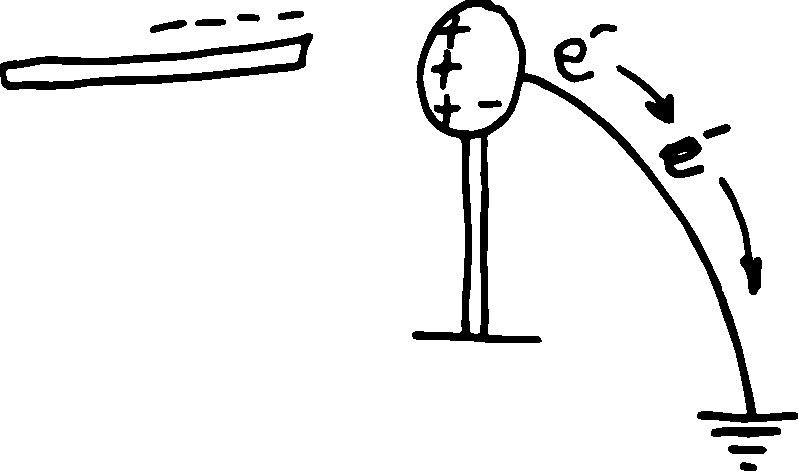
\includegraphics[height=3cm]{01-force-electrique/figures/charge-induction-3.pdf}
  \end{center}


%\paragraph{Matériel}

%\begin{enumerate}
  %\item Ballon
  %\item Balance à torsion pour loi de Coulomb
%\end{enumerate}


%\subsection*{Démonstration de la loi de Coulomb}
%\marginpar{15 minutes}
%\marginpar{Montage installé au labo}

  %Une boule métallique installée sur une balance à torsion.

  %Faire les manips suivantes dans l'ordre.

  %\begin{itemize}
    %\item Boules non chargées, mesurer position du laser et distance entre les
      %boules
    %\item Une boule chargée, mêmes mesures. La boule suspendue devrait se
      %rapprocher de la boule fixe puisqu'elle se polarise par induction.
    %\item Deux boules chargées. La boule suspendue devrait s'éloigner de la
      %boule fixe car des charges de même signe se repoussent. Disons que la
      %distance entre les boules est $r$ et la position du laser s'est déplacée
      %de $d$.
    %\item Si on déplace la boule fixe à $2r$, la force de répulsion entre les
      %deux boules diminue d'un facteur $4$ et le laser devrait être à une
      %distance $d/4$ de sa position d'équilibre.
    %\item On remet la boule fixe à sa position initiale,$r$. On touche la boule
      %fixe avec une troisième boule identique qu'on retire. La charge de la boule fixe passe
      %donc de $Q$ à $Q/2$. La force entre les deux boules diminue donc de
      %moitié et on devrait voir le pointeur laser se déplacer à $d/2$.
  %\end{itemize}

\newpage

\section{Loi de Coulomb}

\marginpar{Tremblay \S 1.9}

\paragraph{Objectif}

\begin{enumerate}
  \item L'étudiant comprendra la loi de Coulomb et comment cette loi capture
    toutes les observations faites précédemment au sujet des charges.
  \item L'étudiant pourra faire des calculs de forces électrostatiques.
  \item L'étudiant comprendra le principe de superposition.
\end{enumerate}


\subsection*{Observations clés}
\marginpar{10 minutes}
  \begin{itemize}
    \item charges opposées s'attirent
    \item charges de même signe se repoussent
    \item plus la charge est grande, plus la force est grande
    \item plus les charges sont éloignées, plus la force est petite
  \end{itemize}

  La loi de Coulomb capture tous ces éléments.

  Considérons deux charges $q_1$ et $q_2$ séparées d'une distance $r$.

    \begin{center}
    \begin{tikzpicture}[
      charge/.style={circle, draw=black!80, fill=black!10, thick}]
      \draw[dashed] (0, 2) -- (4, 0);
      \node[charge] (q1) at (0.8, 1.6) {$q_1$};
      \node[charge] (q2) at (3.2, 0.4) {$q_2$};
      \draw[|<->|] (1.1, 2.2) -- node[fill=white] {$r$} (3.5, 1);
      \draw[ultra thick, ->] (q1) -- node[near end, below] {$\vec{F}_{1
          \leftarrow 2}$} (-0.5, 2.25);
      \draw[ultra thick, ->] (q2) -- node[near end, below]
      {$\vec{u}_{2 \rightarrow 1}$} (2.4, 0.8);
    \end{tikzpicture}
    \end{center}
  On doit avoir
  \begin{eqnarray*}
    F_{1 \leftarrow 2} & \propto & \abs{q_1}, \\
    F_{1 \leftarrow 2} & \propto & \abs{q_2}, \\
    F_{1 \leftarrow 2} & \propto & \frac{1}{r^\gamma}.
  \end{eqnarray*}
  Autrement dit,
  $$
    F_{1 \leftarrow 2} = \frac{k\abs{q_1 q_2}}{r^\gamma}.
  $$
  où $k$ est une constante de proportionnalité. L'exposant peut être trouvé
  expérimentalement. C'est ce qu'à fait Charles Augustin de Coulomb. L'exposant
  est $2$, soit le même que celui qui apparaît dans la loi de la gravitation
  newtonienne.

  Pour spécifier l'orientation, nous utilisons un vecteur unitaire $\vec{u}_{2
  \rightarrow 1}$ qui pointe de la charge $q_2$ vers la charge $q_1$. Si les
  deux charges sont de même signe, la force est répulsive et la force sur $q_1$
  est dans la même direction que $\vec{u}_{2 \rightarrow 1}$. On note que
  $q_1q_2$ est positif. Donc
  $$\vF_{1 \leftarrow 2} = \frac{kq_1q_2}{r^2}\vec{u}_{2 \rightarrow 1}$$

  Trouver les unités par analyse dimensionnelle.
  $$k = \frac{1}{4\pi\epsilon_0} = \SI{8.99e9}{N m^2 / C^2}$$
  $$\epsilon_0 = \SI{8.854e-12}{C^2 / N m^2}$$



\subsection*{Exercice}
\marginpar{20 minutes}
  Deux charges immobiles $q_1 = \SI{4.00}{nC}$ et $q_2 = \SI{-6.00}{nC}$ sont
  situées à \SI{5}{cm} l'une de l'autre.
  Est-il possible de placer une troisième charge le long de la droite reliant
  $q_1$ et $q_2$ de telle sorte qu'elle soit à l'équilibre?


\sectionline


\paragraph{Solution}

D'abord, on fait un schéma de la situation. Imaginons que la charge qu'on
ajoute est positive. La direction de la force exercée par $q_1$ et $q_2$ dans
différentes régions est indiquée sur la figure.

\begin{center}
\begin{tikzpicture}[
      charge/.style={circle, draw=black!80, fill=black!10, thick}]
  \draw[->] (-2, 0) -- (4, 0) node[below] {$x$};
  \node[circle, positive] (q1) at (0, 0.5) {$q_1$};
  \node[circle, negative] (q2) at (3, 0.5) {$q_2$};
  \node[charge] (q) at (-1.5, 0.5) {$q$};
  \draw (q1|-0,0) -- ++(0, -0.2) node[below] {$0$};
  \draw (q2|-0,0) -- ++(0, -0.2) node[below] {$d$};
  \draw (q|-0,0) -- ++(0, -0.2) node[below] {$x$};
  % Forces by q1
  \draw[ultra thick, ->, positive] (-0.3, 1.2) -- ++(-1, 0);
  \draw[ultra thick, ->, positive] (1, 1.2) -- ++(1, 0);
  \draw[ultra thick, ->, positive] (3.3, 1.2) -- ++(1, 0);
  % Forces by q2
  \draw[ultra thick, ->, negative] (-1.3, 1.5) -- ++(1, 0);
  \draw[ultra thick, ->, negative] (1, 1.5) -- ++(1, 0);
  \draw[ultra thick, ->, negative] (4.3, 1.5) -- ++(-1, 0);
\end{tikzpicture}
\end{center}

À gauche de $q_1$, les deux forces sont opposées et la plus grande charge en
valeur absolue est plus éloignée. Il est possible que les deux forces
s'annulent.

Entre $q_1$ et $q_2$, les deux forces sont dans la même direction : elles ne
peuvent pas s'annuler.

À droite de $q_2$, les deux forces sont opposées et la plus grande charge en
valeur absolue est plus proche. Il est impossible que les deux forces
s'annulent.

On conclut donc que la position recherchée est pour une valeur $x$ négative. La
distance entre la nouvelle charge $q$ et $q_1$ est donc $\abs{x}$ alors que la
distance entre $q$ et $q_2$ est de $d - x$. On peut calculer le module de la
force exercée par $q_1$ et $q_2$ sur $q$ ainsi que les composantes.
\begin{align*}
  F_1 &= \frac{k\abs{q_1q}}{x^2}        &  F_{1x} &= -\frac{kq_1q}{x^2} \\
  F_2 &= \frac{k\abs{q_2q}}{(d - x)^2}  &  F_{2x} &= -\frac{kq_2q}{(d - x)^2}
\end{align*}

La force nette sur $q$ est nulle car on veut que cette particule soit à
l'équilibre.  Par le principe de superposition, la force nette sur $q$ est
\begin{align*}
     F_x &= F_{1x} + F_{2x} \\
         &= 0  \\
  F_{1x} &= -F_{2x} \\
  -\frac{kq_1q}{x^2} &= \frac{kq_2q}{(d - x)^2} \\
  -\frac{q_1}{x^2} &= \frac{q_2}{(d - x)^2} \\
  x^2q_2 + q_1(d - x)^2 &= 0 \\
  x^2q_2 + q_1d^2 - 2q_1dx + q_1x^2 &= 0 \\
  (q_1 + q_2) x^2 - 2 q_1 d x + q_1d^2 &= 0 \\
  x &= \frac{2q_1 d \pm \sqrt{4q_1^2d^2 - 4(q_1 + q_2) q_1 d^2}}{2(q_1 + q_2)}
\end{align*}
Les deux réponses possibles sont $x = \SI{-22.25}{cm}$ et $x = \SI{2.247}{cm}$.
On sait que la particule doit être à gauche de $q_1$, donc la bonne solution
est $x = \SI{-22.25}{cm}$.



\subsection*{Exercice}

  \textit{Cet exemple rappelle le principe de superposition.}

  On considère l'ensemble de charges représenté ci-dessous. Les charges sont
  immobiles.

  \begin{center}
  \begin{tikzpicture}[scale=1]
    \node[circle, positive] at (0, 2) (q1) {$q_1$};
    \node[circle, positive] at (0, 0) (q2) {$q_2$};
    \node[circle, positive] at (5, 0) (q3) {$q_3$};
    \node[circle, positive] at (5, 2) (q4) {$q_4$};
    \draw[<->] (q1) -- node[fill=white] {$l$} (q2);
    \draw[<->] (q2) -- node[fill=white] {$d$} (q3);
  \end{tikzpicture}
  \end{center}

  \begin{enumerate}
    \item Trouver une expression algébrique qui représente la force
      électrostatique nette exercée sur la charge $q_4$.
    \item Si $q_1 = \SI{32.8}{nC}$, $q_2 = \SI{1.34}{\micro C}$, $q_3 =
      \SI{-234}{nC}$, $q_4 = \SI{78.6}{nC}$, $l = \SI{0.314}{mm}$ et $d =
      \SI{2.13}{mm}$, déterminer la force électrostatique nette exercée sur la
      charge $q_4$.
  \end{enumerate}


\subsection*{Solution}

\marginpar{25 minutes}

  \begin{center}
  \begin{tikzpicture}[scale=1]
    \draw[->] (-1, -1) -- ++(2, 0) node[below] {$x$};
    \draw[->] (-1, -1) -- ++(0, 2) node[left] {$y$};
    \node[circle, positive] at (0, 2) (q1) {$q_1$};
    \node[circle, positive] at (0, 0) (q2) {$q_2$};
    \node[circle, positive] at (5, 0) (q3) {$q_3$};
    \node[circle, positive] at (5, 2) (q4) {$q_4$};
    \draw[->] (q1) -- ($(q1) ! 0.2 ! (q4)$) node[above] {$\vec{u}_1$};
    \draw[->] (q2) -- ($(q2) ! 0.2 ! (q4)$) node[above] {$\vec{u}_2$};
    \draw[->] (q3) -- ($(q3) ! 0.5 ! (q4)$) node[right] {$\vec{u}_3$};
    \draw[thick, ->] (q4) -- ($(q1) ! 1.4 ! (q4)$) node[above] {$\vec{F}_1$};
    \draw[thick, ->] (q4) -- ($(q2) ! 1.4 ! (q4)$) node[above] {$\vec{F}_2$};
    \draw[thick, ->] (q4) -- ($(q3) ! 1.8 ! (q4)$) node[right] {$\vec{F}_3$};
    \draw[dashed] (q2) -- ++(1.5, 0);
    \draw ($(q2) + (0.7, 0)$) arc (0:20:0.7);
    \node at (0.9, 0.14) {$\theta$};
  \end{tikzpicture}
  \end{center}

  Par la loi de Coulomb

  \begin{align*}
    \vF_1 &= \frac{kq_1q_4}{d^2}\vu_1 & \vu_1 &= \xhat \\
    \vF_2 &= \frac{kq_2q_4}{(l^2 + d^2)}\vu_2 & \vu_2 &= \cos\theta \xhat +
             \sin\theta \yhat \\
    & & &= \frac{d}{\sqrt{l^2 + d^2}} \xhat + \frac{l}{\sqrt{l^2 + d^2}} \yhat \\
    \vF_3 &= \frac{kq_3q_4}{l^2}\vu_3 & \vu_3 &= \yhat \\
  \end{align*}

  Par le principe de superposition, la force nette sur $q_4$ est

  \begin{align*}
    \vF &= \vF_1 + \vF_2 + \vF_3 \\
        &= \frac{kq_1q_4}{d^2}\xhat +
           \frac{kq_2q_4}{(l^2 + d^2)} \left( \frac{d}{\sqrt{l^2 + d^2}} \xhat + \frac{l}{\sqrt{l^2 + d^2}} \yhat \right) +
           \frac{kq_3q_4}{l^2}\yhat \\
        &= kq_4\left[ \frac{q_1}{d^2} + \frac{q_2 d}{(l^2 + d^2)^{3/2}} \right] \xhat
         + kq_4\left[ \frac{q_3}{l^2} + \frac{q_2 l}{(l^2 + d^2)^{3/2}} \right] \yhat
  \end{align*}

  Pour l'application numérique, il suffit de remplacer les valeurs numériques:

  \begin{align*}
    \vF &= (\SI{8.99e9}{Nm^2/C^2}) (\SI{78.6}{nC})
          \left[ \frac{\SI{32.8}{nC}}{(\SI{2.13}{mm})^2} +
            \frac{(\SI{1.34}{\micro\coulomb}) (\SI{2.13}{mm})}{((\SI{0.314}{mm})^2
              + (\SI{2.13}{mm})^2)^{3/2}} \right] \xhat \\
        &{} + (\SI{8.99e9}{Nm^2/C^2}) (\SI{78.6}{nC})
          \left[ \frac{\SI{-234}{\nano C}}{(\SI{0.314}{mm})^2} +
            \frac{(\SI{1.34}{\micro\coulomb}) (\SI{0.314}{mm})}{((\SI{0.314}{mm})^2
              + (\SI{2.13}{mm})^2)^{3/2}} \right] \yhat
  \end{align*}
  Ce qui donne
  \[
    \boxed{\vF = \SI{207.2}{N}\xhat - \SI{1647}{N}\yhat}
  \]



\sectionline

\section{Questions de révision}

\subsection*{Exemple}
\marginpar{10 minutes}
\marginpar{Diapo}
  On place une particule chargée à l'intérieur d'une sphère métallique creuse.
  À proximité, on place un pendule dont l'extrémité est métallique. Que se
  passe-t-il?

  \begin{center}
    \begin{tikzpicture}
      \draw[orange, fill=orange!20] (4, 1.5) -- (4, 0) -- (5, 0) -- (5, 1.5);
      \draw[ultra thick, fill=white] (4.5, 2) circle[radius=1];
      \node[circle, draw=black!70, fill=black!10] at (4.5, 2.0) {$+$};
      \node[circle, draw=black!80, fill=black!40, minimum size=6mm] (bob)
        at (0.7, 2.2) {};
      \draw[ultra thick] (-1.5, 0) -- (-1.5, 3) -- (0, 3);
      \draw (0, 3) -- (bob);
      \node at ($(bob) + (0.15, 0.13)$) {$-$};
      \node at ($(bob) + (0.15, -0.13)$) {$-$};
      \node at ($(bob) + (-0.15, 0.13)$) {$+$};
      \node at ($(bob) + (-0.15, -0.13)$) {$+$};
      \draw[decorate, decoration={markings,
                      mark=between positions 0 and 1 step 5.1mm with {
                         \node (0, 0) {$-$};}}] (4.5, 2) circle[radius=0.8];
      \draw[decorate, decoration={markings,
                      mark=between positions 0 and 1 step 6mm with {
                         \node (0, 0) {$+$};}}] (4.5, 2) circle[radius=1.2];
    \end{tikzpicture}
  \end{center}



\section*{Exercices supplémentaires}

\subsection*{Loi de Coulomb 1D}

  Deux amis jouent dans la ruelle. Ils tiennent chacun une sphère chargée. La
  masse combinée de Luc et de sa sphère est de \SI{62.3}{kg}, celle de Corinne
  est de \SI{58.7}{kg}. La charge portée par la sphère de Luc est de
  \SI{481}{\mu C} et celle portée par la sphère de Corinne est de \SI{965}{\mu C}.

  Lorsque les deux amis sont séparés de \SI{2}{m}, quelle est l'accélération
  subie par Luc?

  \begin{center}
    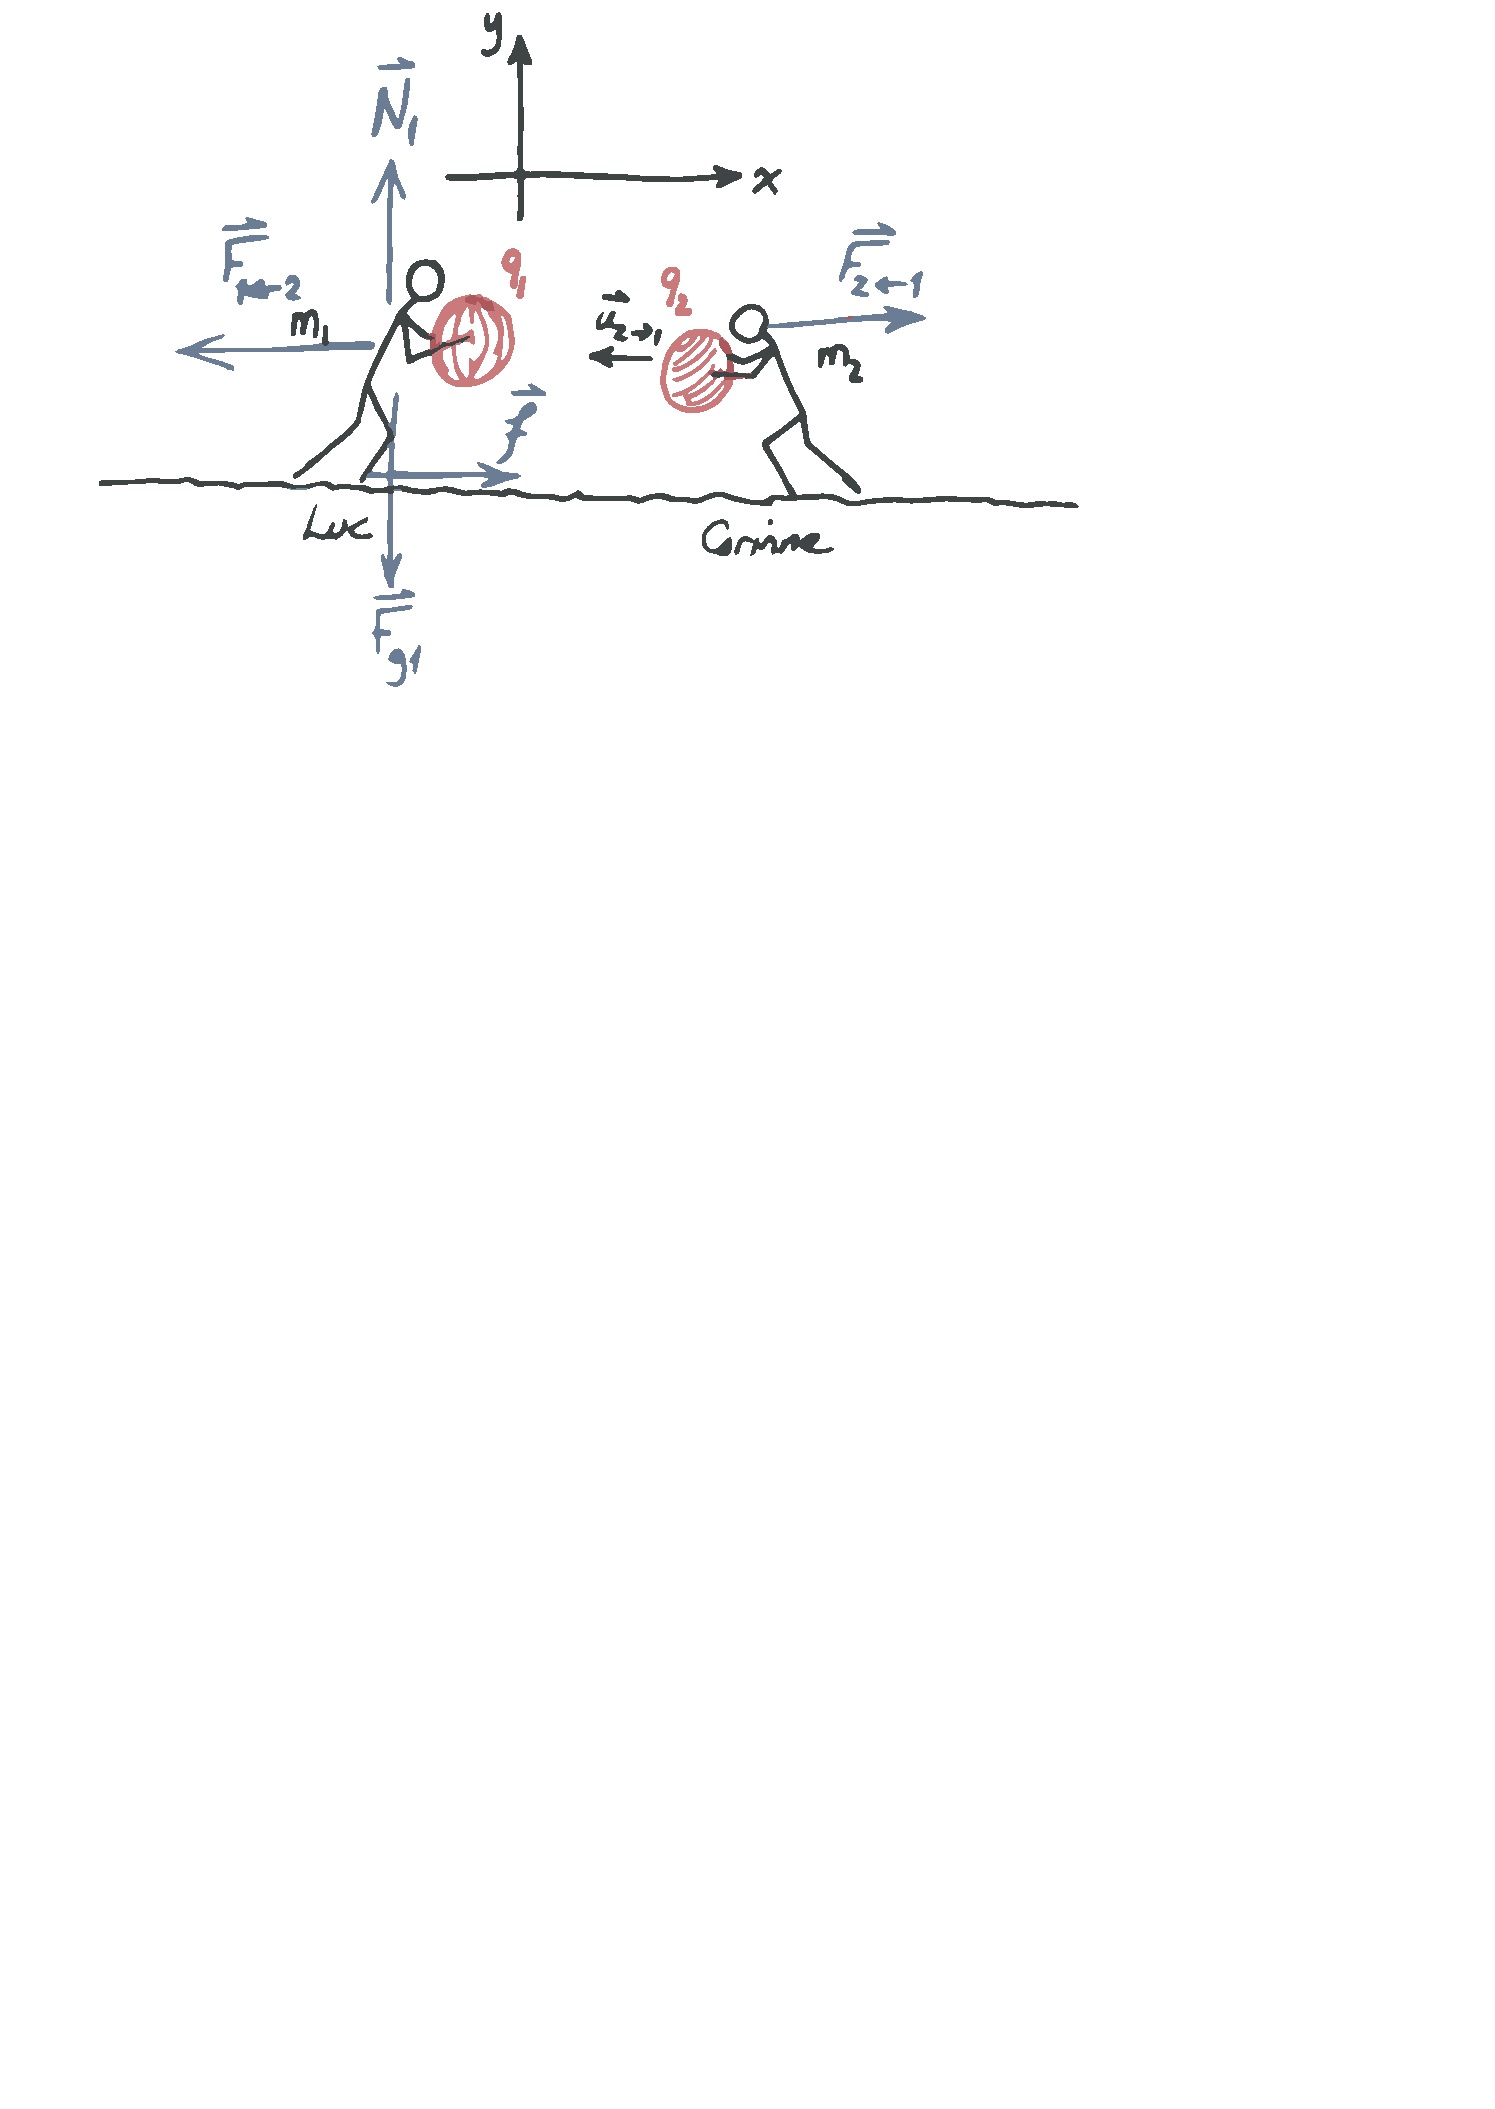
\includegraphics[scale=0.45]{01-force-electrique/figures/pousse-charge-soln-dessin.pdf}
  \end{center}
  
  Par la deuxième loi de Newton, $\vF_1 = m_1 \va_1$. Sachant que
  l'accélération en $y$ est nulle, on obtient

  \begin{align}
    \text{En } y \text{ : } & N_1 - m_1g = 0
    &  \text{En } x \text{ : } & -F_{12} + f_c = m_1 a_{1x}  \nonumber \\
    & N_1 = m_1 g
    & & -F_{12} + \mu_c N_1 = m_1 a_{1x}  \nonumber \\
    & & & -F_{12} + \mu_c m_1 g = m_1 a_{1x}
    \label{eq:exsupp_coulomb1d_1}
  \end{align}

  Par la loi de Coulomb, la force électrique est
  \begin{align*}
    \vF_{12} &= \frac{kq_1q_2}{r^2} \vu_{2\rightarrow 1} \\
             &= \frac{kq_1q_2}{r^2} (-\xhat)
  \end{align*}
  Dans \ref{eq:exsupp_coulomb1d_1}
  \begin{align*}
    -\frac{kq_1q_2}{r^2} + \mu_c m_1 g &= m_1 a_{1x}  \\
    a_{1x} &= -\frac{kq_1q_2}{m_1r^2} + \mu_c g 
  \end{align*}
  Avec une valeur raisonnable du frottement entre les souliers de Luc et le sol
  de $\mu_c = \num{0.6}$, on obtient
  \[
    \boxed{\va_1 = \SI{-10.86}{m/s^2}\xhat}
  \]


\subsection*{Loi de Coulomb 2D}

  On considère trois charges $q_1 = Q$, $q_2 = -2Q$ et $q_3 = 2Q$ placées aux
  sommets d'un triangle équilatéral de côté $d$. Une quatrième charge $q_4 =
  -Q$ est placée au centre du triangle. Déterminer la force électrostatique qui
  agit sur la charge centrale.

  La situation est illustrée ci-dessous.

  \begin{center}
  \begin{tikzpicture}
    \coordinate (center) at (2, 1.155);
    \coordinate (p1) at (2, 3.464);
    \coordinate (p2) at (0, 0);
    \coordinate (p3) at (4, 0);
    \path[fill=black!5] (0,0) -- ($(p2)!(p1)!(p3)$) -- (center) -- cycle;
    \node[circle, negative, minimum size=12mm] (q2) at (0, 0) {$-2Q$};
    \node[circle, positive, minimum size=12mm] (q1) at (2, 3.464) {$Q$};
    \node[circle, positive, minimum size=12mm] (q3) at (4, 0) {$2Q$};
    \draw (q2) -- (q3) -- (q1) -- (q2);
    \draw[dashed] (q2) -- ($(q1)!(q2)!(q3)$);
    \draw[dashed] (q1) -- ($(q2)!(q1)!(q3)$);
    \draw[dashed] (q3) -- ($(q1)!(q3)!(q2)$);
    \node[circle, draw=black!80, thick, fill=black!10] (q4) at (center) {$q_4$};
    \draw[ultra thick, ->] (q4) -- ($0.66*(q4) + 0.66*(q1)!(q2)!(q3)$);
    \draw[ultra thick, ->] (q4) -- ($0.34*(q4) + 0.66*(q3)$);
    \draw[ultra thick, ->] (q4) -- ($0.6*(q4) + 0.4*(q1)$);
  \end{tikzpicture}
  \end{center}

  Soit $\vec{F}_1$, $\vec{F}_2$ et $\vec{F}_3$ les forces électrostatiques sur
  $q_4$ dues à $q_1$, $q_2$ et $q_3$, respectivement. Puisque $q_2$ et $q_3$
  ont une charge identique en valeur absolue et sont à la même distance de
  $q_4$, les grandeurs $\vec{F}_2$ et $\vec{F}_3$ ont identiques. De plus, la
  symétrie du triangle équilatéral implique que les composantes horizontales de
  ces deux forces sont identiques et que les composantes verticales s'annulent.
  Par conséquent,
  \begin{eqnarray*}
    \vec{F}_2 + \vec{F}_3 &= 2 \cos\left( \frac{\pi}{6} \right)k
      \frac{2Q^2}{r^2}\xhat \\
    &= \frac{\sqrt{3} Q^2}{2\pi\varepsilon_0 r^2} \xhat
  \end{eqnarray*}
  où $r$ est la distance entre le centre du triangle et un de ses sommets.
  vertices, and $\xhat$ is a unit vector pointing right. À partir du triangle
  ombragé dans la figure ci-dessous, on trouve
  \begin{equation*}
    r^2 = \frac{d^2}{3}
  \end{equation*}
  ce qui implique que
  \begin{equation*}
    \vec{F}_2 + \vec{F}_3 = \frac{3\sqrt{3} Q^2}{2\pi\varepsilon_0 d^2} \xhat.
  \end{equation*}
  $\vec{F}_1$ a seulement une composante verticale
  \begin{eqnarray*}
    \vec{F}_1 &= k \frac{Q^2}{r^2} \yhat \\
    &= k \frac{3Q^2}{d^2} \yhat
  \end{eqnarray*}
  où $\yhat$ est un vecteur unitaire qui pointe vers le haut.
  La force sur $q_4$ est donc
  \begin{equation*}
    \vec{F} = \vec{F}_1 + \vec{F}_2 + \vec{F}_3 =
    \frac{3Q^2}{2\pi\varepsilon_0 d^2} \left( \sqrt{3} \xhat + \frac{1}{2}\yhat
    \right).
  \end{equation*}

%\chapter{Champ électrique}

\section{Qu'est-ce que le champ électrique?}

\marginpar{Tremblay \S 2.1}


\paragraph{Objectif}
\begin{enumerate}
  \item L'étudiante comprendra ce qu'est un champ électrique.
  \item Elle pourra calculer le champ électrique produit par un ensemble de
    charges ponctuelles en appliquant le principe de superposition.
\end{enumerate}


\marginpar{5 minutes}
  Le concept d'action à distance est troublant. La loi de Coulomb suggère que
  si deux charges interagissent et que l'une des deux se déplace, l'autre
  subira les effets instantanément. Or, cela voudrait dire qu'il est possible
  de faire voyager de l'information plus vite que la vitesse de la lumière. De
  plus, des expériences minutieuses confirment qu'il y a un délai avant que la
  deuxième charge ne détecte un changement de la position de la première. Ce
  délai est de l'ordre de \SI{1e-8}{s} pour deux charges séparées d'environ
  \SI{1}{m}.

  Il faut donc un intermédiaire entre les deux charges. Cet intermédiaire est
  le \textbf{champ électrique}. Un objet chargé génère autour de lui un
  champ électrique.


\subsection*{Analogie avec le champ gravitationnel}
\marginpar{5 minutes}

Selon la loi de la gravitation universelle de Newton
\[
  F_g = \frac{Gm_1m_2}{r^2}.
\]
La partie $Gm_1 / r^2$ ne dépend que de la source du champ gravitationnel et de
la distance entre le centre de masse de cet objet et le point où on veut
calculer la force. Par exemple, à la surface de la Terre on a
\[
  \frac{GM_\oplus}{R_\oplus^2} = \SI{9.8}{m/s^2} \equiv g
\]
et on peut calculer la force sur un objet de masse $m$ à la surface de la Terre
avec
\[
  F_g = mg.
\]
Pour la force électrique, c'est le même principe. À partir de la loi de
Coulomb
\[
  F_e = \frac{k\abs{q_1}\abs{q_2}}{r^2}
\]
on reconnait qu'une partie de l'expression ne dépend que de la source et de la
distance à laquelle on se trouve de cette source
\[
  E = \frac{k\abs{q_1}}{r^2}.
\]
On peut calculer la force sur une particule chargée située à une distance $r$
de $q_1$ en faisant simplement
\[
  F_e = E\abs{q_2}.
\]




\section{Champ électrique d'une charge ponctuelle}
\marginpar{Tremblay \S 2.2}

\marginpar{5 minutes}

  $$\vec{E} = \frac{kq}{r^2} \vec{u}_{r}$$

  où $\vec{u}_r$ est un vecteur unitaire qui s'éloigne de la charge ponctuelle.

  \begin{center}
  \begin{tikzpicture}
    \matrix[column sep=1.5cm] {
    \node[positive, circle] (q) at (0, 0) {$+$};
    \foreach \theta in {0, 30, ..., 330} {
      \draw[->] (q) -- ++(\theta:1);
      \draw[->] ($(q) + (\theta:1.05)$) -- ++(\theta:0.5);
      \draw[->] ($(q) + (\theta:1.05) + (\theta:0.55)$) -- ++(\theta:0.25);
    }
    &
    \node[negative, circle] at (0, 0) {$-$};
    \foreach \theta in {0, 30, ..., 330} {
      \draw[<-] (q) -- ++(\theta:1);
      \draw[<-] ($(q) + (\theta:1.05)$) -- ++(\theta:0.5);
      \draw[<-] ($(q) + (\theta:1.05) + (\theta:0.55)$) -- ++(\theta:0.25);
    }
    \\
    };
  \end{tikzpicture}
  \end{center}



\subsection*{Exercice}
\marginpar{5 minutes}
\marginpar{Diapo}
  Dans chacune des situations ci-dessous, utilisez les informations fournies
  pour trouver la direction du champ électrique à la position de la charge de
  droite.

  \begin{enumerate}
    \item
      \begin{tikzpicture}
        \node[positive, circle] (q1) at (0, 0) {$+$};
        \node[positive, circle] (q2) at (2, 0) {$+$};
      \end{tikzpicture}
    \item
      \begin{tikzpicture}
        \node[positive, circle] (q1) at (0, 0) {$+$};
        \node[negative, circle] (q2) at (2, 0) {$-$};
      \end{tikzpicture}
    \item
      \begin{tikzpicture}
        \node[negative, circle] (q1) at (0, 0) {$-$};
        \node[positive, circle] (q2) at (2, 0) {$+$};
      \end{tikzpicture}
    \item
      \begin{tikzpicture}
        \node[draw, circle] (q1) at (0, 0) {$q$};
        \node[negative, circle] (q2) at (2, 0) {$-$};
        \draw[very thick, ->] (q2) -- ++(1.5, 0) node[right] {$\vec{F}$};
      \end{tikzpicture}
    \item
      \begin{tikzpicture}
        \node[positive, circle] (q1) at (0, 0) {$+$};
        \node[draw, circle] (q2) at (2, 0) {$q$};
        \draw[very thick, ->] (q2) -- ++(-1.5, 0) node[below] {$\vec{F}$};
      \end{tikzpicture}
  \end{enumerate}


\subsection*{Principe de superposition}
\marginpar{5 minutes}

  Le champ électrique total en un point de l'espace est la somme des champs
  électrique causés par toutes les charges à proximité.

  On peut voir que c'est vrai à partir du principe de superposition pour les
  forces électriques.
  \begin{eqnarray*}
    \vF = q\vec{E} &=& \vF_1 + \vF_2 + \cdots + \vF_n \\
          &=& q \vec{E}_1 + q \vec{E}_2 + \cdots + q \vec{E}_n \\
          &=& q \left( \vec{E}_1 + \vec{E}_2 + \cdots + \vec{E}_n \right)
  \end{eqnarray*}



\subsection*{Exercice}
\marginpar{25 minutes}
  Une charge $q = \SI{30}{\micro\coulomb}$ est placée à \SI{160}{cm} du sol. À
  droite de cette charge, une charge $Q = \SI{-50}{\micro\coulomb}$ est placée
  à \SI{2}{m} au-dessus du sol. La distance entre les deux charges est $D =
  \SI{3}{m}$.

  Calculer le champ électrique au point $P$ situé à \SI{1}{m} à droite de la
  charge $q$ et à \SI{4}{m} au-dessus du sol.

  \begin{center}
    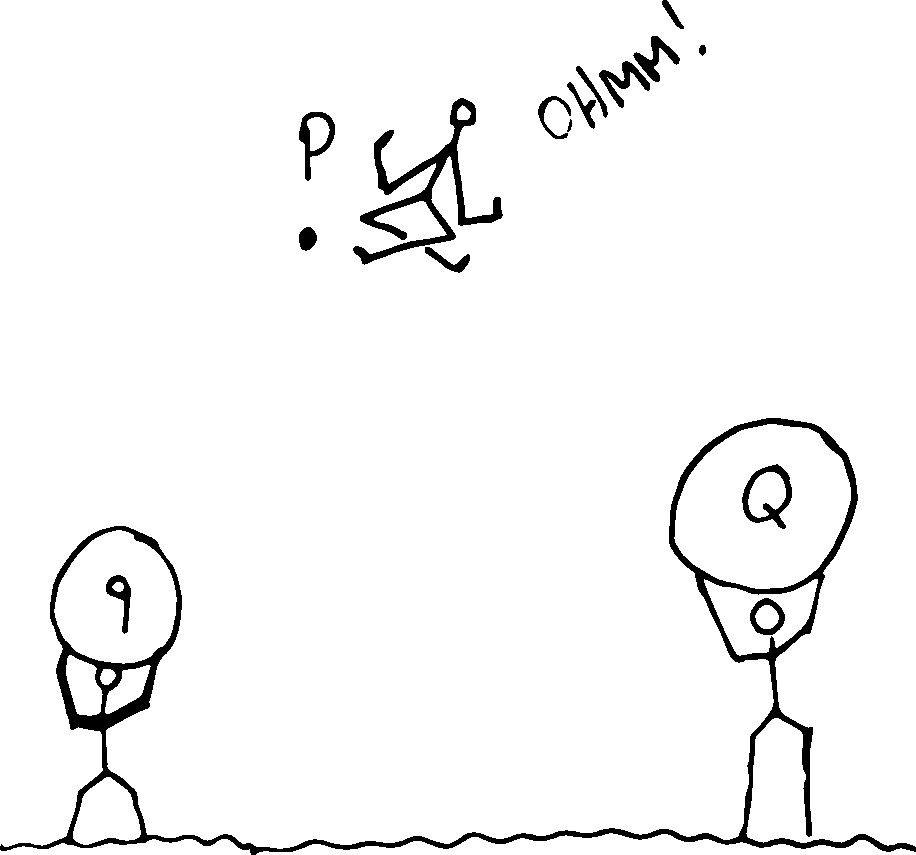
\includegraphics[scale=0.25]{02-champ-electrique/figures/champ-deux-charges-1.pdf}
  \end{center}

  \sectionline

\paragraph{Solution}
  Les coordonnées du point $P$ sont $x = \SI{1}{m}$, $y = \SI{2.4}{m}$.
  \begin{center}
    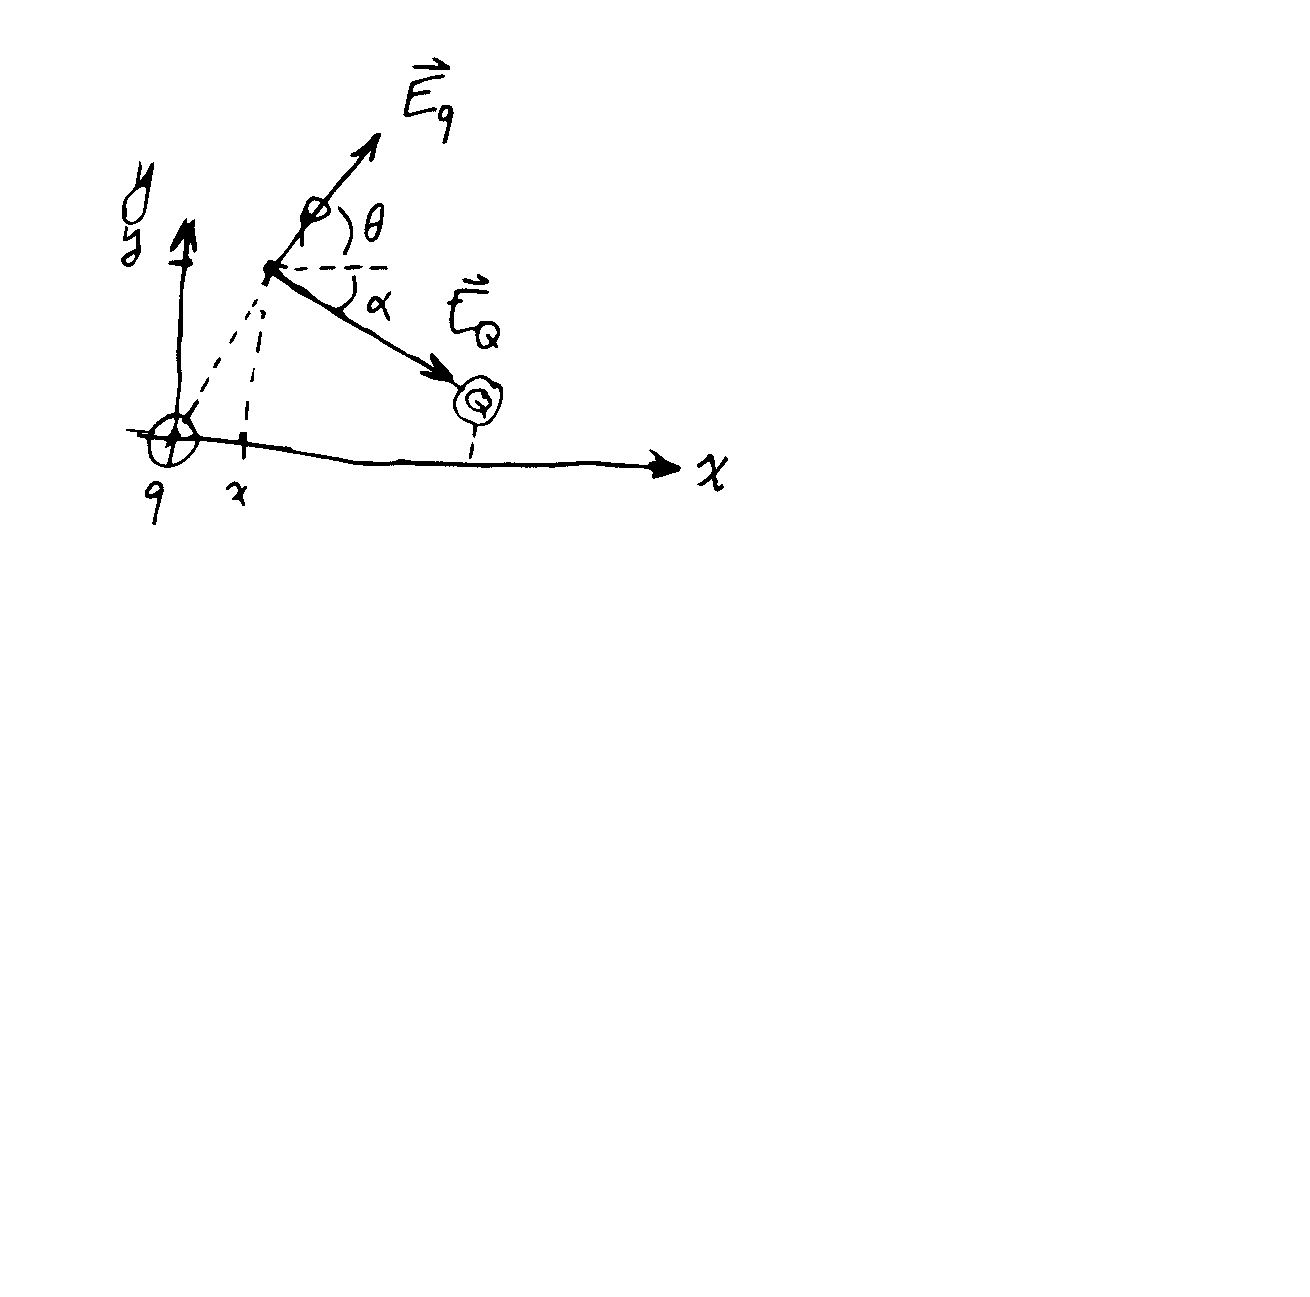
\includegraphics[scale=0.5]{02-champ-electrique/figures/champ-deux-charges-soln.pdf}
  \end{center}
  Le champ électrique de la charge $q$ au point $P$ est de grandeur et
  composantes
  \begin{align*}
    E_q &= \frac{k\abs{q}}{x^2 + y^2} \\
    E_{qx} &= E_q \cos \theta
        &= \frac{k\abs{q}}{x^2 + y^2} \frac{x}{\sqrt{x^2 + y^2}}
        &= \frac{k\abs{q}x}{(x^2 + y^2)^{3/2}}
        &= \SI{15344}{N/C} \\
    E_{qy} &= E_q \sin \theta
        &= \frac{k\abs{q}}{x^2 + y^2} \frac{y}{\sqrt{x^2 + y^2}}
        &= \frac{k\abs{q}y}{(x^2 + y^2)^{3/2}}
        &= \SI{36827}{N/C} \\
  \end{align*}
  Le champ électrique de la charge $Q$ au point $P$ est de grandeur et
  composantes
  \begin{align*}
    E_Q &= \frac{k\abs{Q}}{r_Q^2} \\
    E_{Qx} &= E_Q \cos \alpha
        &= \frac{k\abs{Q}}{r_Q^2} \frac{1}{\sqrt{2}}
        &= \frac{k\abs{Q}}{\sqrt{2}r_Q^2}
        &= \SI{39730}{N/C} \\
    E_{Qy} &= -E_Q \sin \alpha
        &= -\frac{k\abs{Q}}{r_Q^2} \frac{1}{\sqrt{2}}
        &= -\frac{k\abs{Q}}{\sqrt{2}r_Q^2}
        &= \SI{-39730}{N/C} \\
  \end{align*}
  Par le principe de superposition
  \begin{align*}
    \vE &= \vE_q + \vE_Q  \\
        &= \left(\num{55075}\xhat - \num{2903}\yhat\right) \si{N/C}
  \end{align*}



\section{Lignes de champ électrique}
\marginpar{Tremblay \S 2.4}

\paragraph{Objectif}

\begin{enumerate}
  \item L'étudiante connaîtra le lien entre les lignes de champ et le champ
    électrique.
  \item L'étudiante pourra utiliser la notion de champ électrique pour calculer
    la force sur une particule chargée.
\end{enumerate}

\paragraph{Démonstration}
\marginpar{10 minutes}

  Matériel
  \begin{enumerate}
    \item Un vase de Pétri
    \item Huile végétale
    \item Graines de gazon
    \item Source de champ électrique (générateur de Van de Graaff)
    \item Électrodes
    \item Fils
  \end{enumerate}

  Manipulations
  \begin{enumerate}
    \item Mettre de l'huile dans le vase de Pétri
    \item Ajouter les graines de gazon dans l'huile
    \item Connecter un fil à la sphère et un fil à la mise à la terre
    \item Connecter l'autre extrémité des fils aux électrodes
    \item Mettre les électrodes dans l'huile et démarrer le Van de Graaf.
  \end{enumerate}


\subsection*{Caractéristiques des lignes de champ}
\marginpar{10 minutes}

  Les lignes de champ électrique permettent de visualiser le champ électrique.
  Lorsqu'on les trace, on doit respecter les règles suivantes :

  \begin{itemize}
    \item le champ électrique est tangent aux lignes de champ;
    \item la norme du champ électrique est proportionnelles à la densité de
      lignes de champ.
    \item les lignes de champ commence sur les charges positives ou à l'infini
    \item les lignes de champ se termine sur les charges négatives ou à
      l'infini
  \end{itemize}

  \begin{center}
      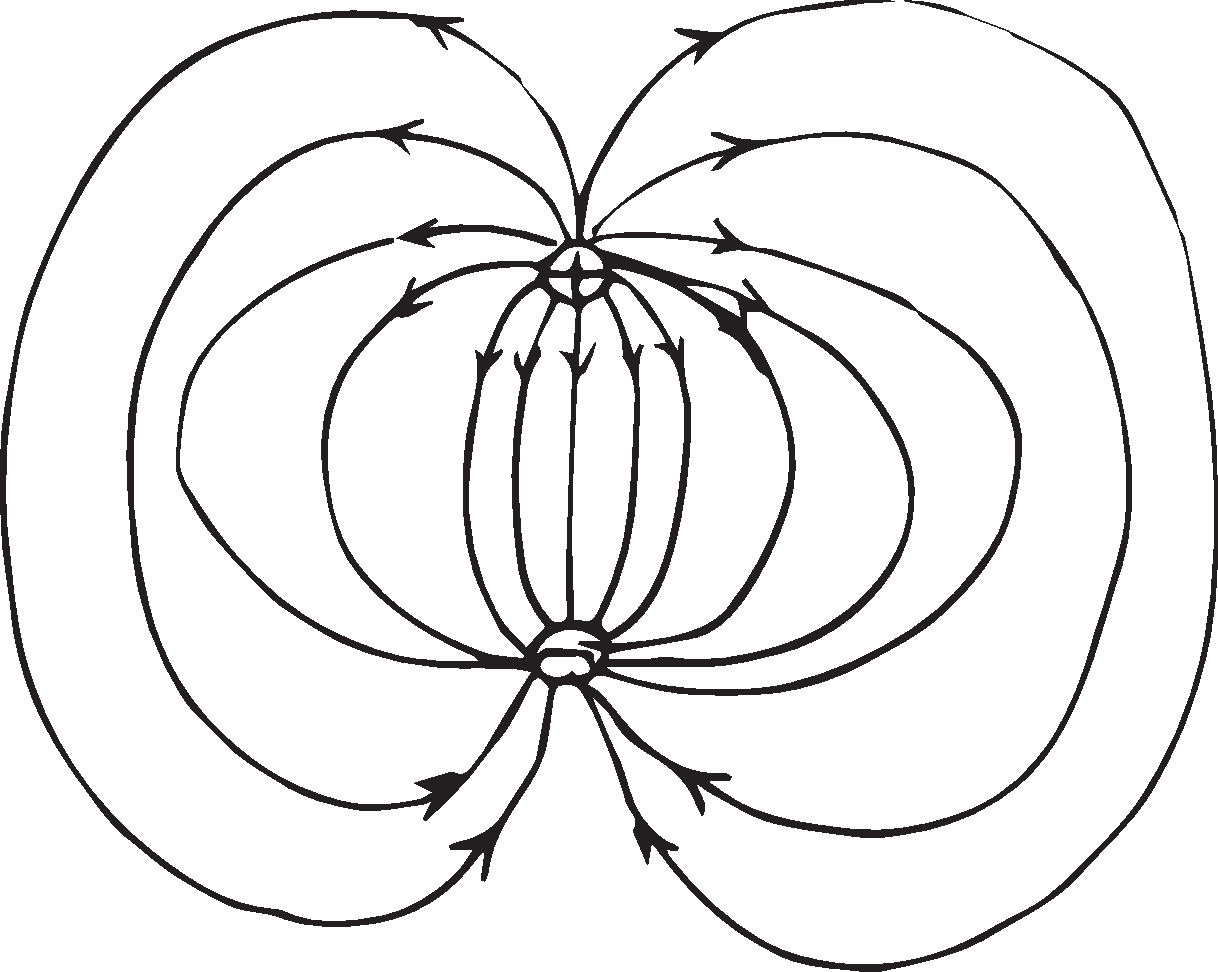
\includegraphics[scale=0.3]{02-champ-electrique/figures/lignes-champ-dipole.pdf}
      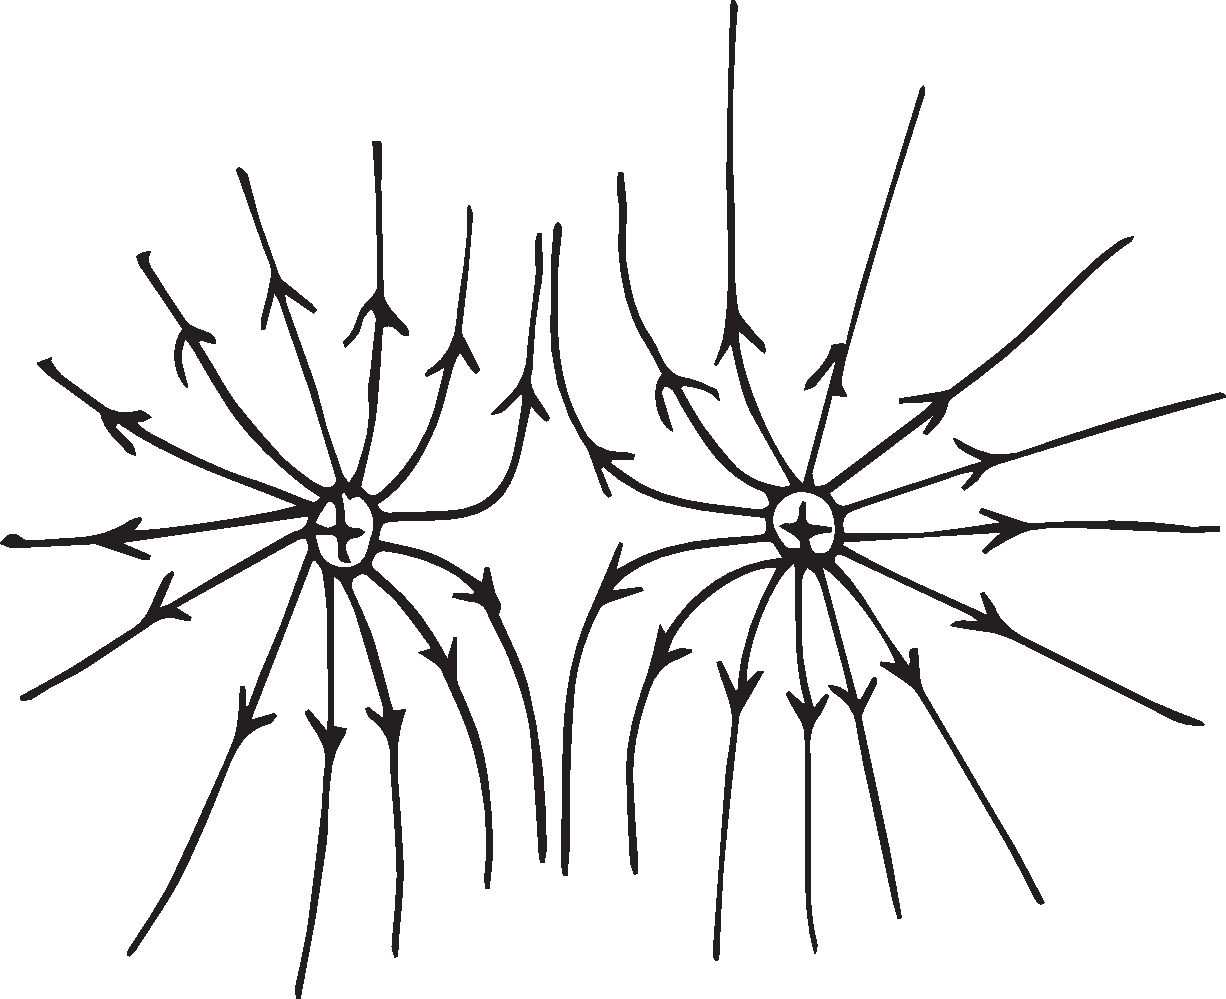
\includegraphics[scale=0.3]{02-champ-electrique/figures/lignes-champ-deux-plus.pdf}
  \end{center}

  Conséquences de ces règles :

  \begin{itemize}
    \item le nombre de lignes de champ qui se terminent ou qui commencent sur une
      charge est proportionnel à la charge;
    \item les lignes de champ ne se croisent jamais.
  \end{itemize}


\sectionline


\section{Mouvement d'une particule chargée dans un champ uniforme}

\marginpar{Tremblay \S 2.6}

\marginpar{5 minutes}

  Si le champ $\vec{E}$ est le même partout dans l'espace on dit qu'il est
  \textbf{uniforme}. Dans un champ uniforme, une particule chargée subit
  une accélération constante. En effet,

  $$\vec{F} = q\vec{E} = m\vec{a}$$

  par la deuxième loi de Newton. Donc

  $$\vec{a} = \frac{q\vec{E}}{m}$$

  est constante.


\subsection*{Tube à rayons cathodiques}
\marginpar{30 minutes}

  Il y a quelques années, téléviseurs et écrans d'ordinateur fonctionnaient
  avec des tubes à rayons cathodiques.

  \begin{center}
    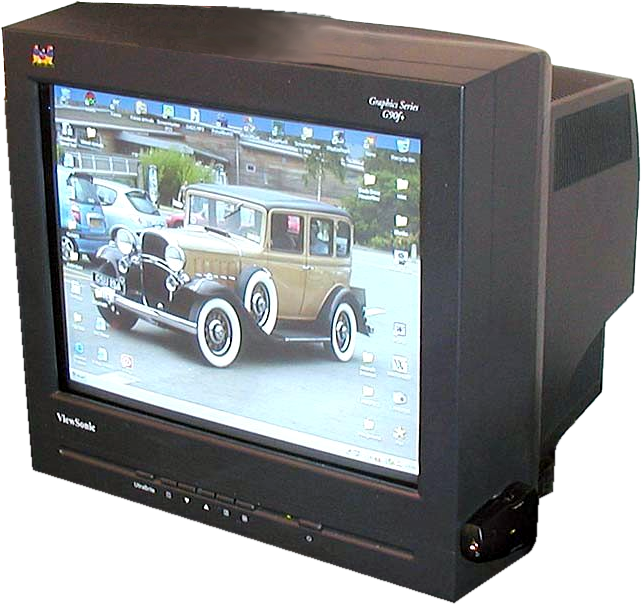
\includegraphics[scale=0.2]{02-champ-electrique/figures/viewsonic-crt.png}
  \end{center}

  Le principe est simple: un élément chauffant produit un faisceau d'électrons
  qui est accéléré dans un champ électrique. Les électrons sont ensuite déviés
  par un autre champ électrique. Lorsqu'ils atteignent l'écran, ils transfèrent
  leur énergie à des phosphores qui produisent de la lumière.

  \begin{center}
  \begin{tikzpicture}[>=stealth, scale=0.8]
    \draw plot[smooth cycle] coordinates {(0, 1) (2, 1.5) (6, 3) (6, -3) (2, -1.5) (0, -1)};
    \draw[ultra thick] (0.8, 0.5) -- (2.5, 0.5);
    \draw[ultra thick] (0.8, -0.5) -- (2.5, -0.5);
    \foreach \x in {1.1, 1.5, 1.9, 2.3} {
      \node at (\x, 0.7) {$+$};
      \node at (\x, -0.7) {$-$};
    }
    \draw[thick, blue] plot[smooth] coordinates {(0, 0) (0.8, 0) (1.2, 0.02) (1.6, 0.04) (2, 0.08) (2.4, 0.16) (2.6, 0.2)} -- (6.4, 1.5);
    \draw[|<->|] (7, 3) -- node[fill=white] {$D$} (7, -3);
    \draw[|<->|] (0.8, -1.1) -- node[fill=white] {$l$} (2.5, -1.1);
    \draw[<->|] (2.5, -1.1) -- node[fill=white] {$L$} (6.4, -1.1);
  \end{tikzpicture}
  \end{center}

  Les plaques métalliques génèrent un champ électrique uniforme $\vec{E}$.
  Les dimensions du tube sont $l = \SI{2}{\centi\meter}$, $L =
  \SI{40}{\centi\meter}$ et $D = \SI{60}{\centi\meter}$.  Avant de passer entre
  les plaques du déflecteur, la vitesse des électrons est
  5\% de la vitesse de la lumière vers la droite.

  Déterminer la norme du champ électrique nécessaire pour que les électrons
  atteignent le haut de l'écran.


  Soit $v_x$ et $v_y$ les composantes horizontales et verticales de la vitesse
  des électrons à leur entrée entre les deux plaques.

  Pas de force dans la direction $x$ donc $v_x$ est constante: $v_x = 0.05c$.

  Le temps requis pour que les électrons traversent les plaques est
  \[
    t_l = \frac{l}{v_x}
  \]

  Pendant la traversée des plaques, les électrons sont soumis à une force
  constante vers le haut dont la grandeur est
  \[
    F = eE
  \]
  où $E$ est la grandeur du champ électrique. Par la deuxième loi de Newton
  \[
    a_y = \frac{eE}{m}.
  \]
  La composante verticale de la vitesse à la sortie des plaques est donc
  \[
    v_{yl} = \frac{eE t_l}{m} = \frac{eEl}{mv_x}
  \]
  Le déplacement vertical pendant le passage entre les plaques est
  \begin{eqnarray*}
    y_l &=& \frac{1}{2} a_y t_l^2 \\
    &=& \frac{1}{2} \frac{eE}{m} \frac{l^2}{v_x^2} \\
    &=& \frac{eEl^2}{2mv_x^2}
  \end{eqnarray*}
  Pour la partie après les plaques, il n'y a pas de force, donc vitesse
  constante.
  \[
    t_L = \frac{L}{v_x}
  \]
  et
  \begin{eqnarray*}
    y_L &=& v_{yl} t_L \\
    &=& \frac{eEl}{mv_x}\frac{L}{v_x} \\
    &=& \frac{eElL}{mv_x^2}.
  \end{eqnarray*}
  Pour atteindre le haut de l'écran, $y_L = D/2$ donc
  \begin{eqnarray*}
    \frac{D}{2} &=& \frac{eEl^2}{2mv_x^2} + \frac{eElL}{mv_x^2} \\
     &=& \frac{eEl}{mv_x^2} \left(\frac{l}{2} + L\right) \\
    E &=& \frac{Dmv_x^2}{2el (l/2 + L)} = \SI{46.7}{kN/C}
  \end{eqnarray*}


\sectionline


\section{Distributions de charge}

\marginpar{Tremblay \S 2.5}

\paragraph{Objectif}

\begin{enumerate}
  \item L'étudiant pourra calculer le champ électrique produit par une
    distribution de charge.
  \item L'étudiant comprendra qu'on peut diviser un objet étendu en petits
    morceau, considérer ces morceaux comme des particules, puis additionner les
    contributions de ces morceaux pour obtenir l'effet total.
  \item L'étudiant pourra utiliser le calcul intégral pour résoudre des
    problèmes de calcul de champ électrique.
\end{enumerate}


\subsection*{Exercice d'introduction aux distributions de charge}

\marginpar{10 minutes}

Chaque disque et l'anneau ont tous la même charge $Q$.
Classer les objets en ordre croissant de la grandeur du champ électrique au
point $P$.

\begin{center}
\begin{tikzpicture}
  \matrix[row sep=1em, column sep=1em] {
  \node at (0, -2.5) {(a)};
  \draw (0, 1.5) circle(1pt);
  \node[left] at (0, 1.5) {$P$};
  \draw (0,-2) -- (0,0);
  \draw[fill=black!10] (0,0) ellipse[x radius=1, y radius=0.5];
  \draw (0,0) -- (0,2);
  \draw (0,0) -- ++(-30:0.75);
  \node at (5:0.5) {$R$}; &
  \node at (0, -2.5) {(b)};
  \draw (0, 1.5) circle(1pt);
  \node[left] at (0, 1.5) {$P$};
  \draw (0,-2) -- (0,0);
  \draw[fill=black!10] (0,0) ellipse[x radius=2, y radius=1];
  \draw (0,0) -- (0,2);
  \draw (0,0) -- ++(-30:1.5);
  \node at (-05:0.8) {$2R$}; &
  \draw (0, 1.5) circle(1pt);
  \node[left] at (0, 1.5) {$P$};
  \node at (0, -2.5) {(c)};
  \draw (0,-2) -- (0,0);
  \draw[fill=black!10] (0,0) ellipse[x radius=2, y radius=1];
  \draw[fill=white] (0,0) ellipse[x radius=1, y radius=0.5];
  \draw (0,-0.5) -- (0,2);
  \draw (0,0) -- ++(-150:0.75);
  \node at (180:0.5) {$R$};
  \draw (0,0) -- ++(-30:1.5);
  \node at (-10:1.4) {$2R$};\\
  };
\end{tikzpicture}
\end{center}


\subsection*{Calcul de champ le long de l'axe d'une tige chargée}

\marginpar{20 minutes}

Comment peut-on calculer le champ électrique produit par un objet chargé qui
n'est pas ponctuel? La formule que nous avons vue ne s'applique pas.

Nous allons d'abord considérer une tige chargée (ou un fil) de longueur $L$
portant une charge totale $Q$ répartie uniformément dans la tige.

Un fil n'est pas une particule ponctuelle, mais on peut le subdiviser en petits
morceaux.

Un segment de longueur $\Delta x$ porte une fraction de la charge totale.

\paragraph{Question}: quelle fraction de la charge $Q$ est portée par un
segment de longueur $\Delta x$?

\begin{eqnarray*}
\Delta q &=& Q \frac{\Delta x}{L} \\
         &=& \frac{Q}{L} \Delta x
\end{eqnarray*}

On appelle le rapport $Q/L$ une  \textbf{densité linéique de charge}. On
utilise souvent le symbole $\lambda$ pour représenter une densité linéique
$$\lambda = \frac{Q}{L}$$
dans le cas d'une tige chargée uniformément.

Donc
$$\Delta q = \lambda \Delta x.$$

Si $\Delta x$ est suffisamment petit, on peut considérer ce morceau de fil
comme une charge ponctuelle. Le champ électrique généré par ce bout de fil est
donc
\begin{eqnarray*}
\Delta E_x &\approx& \frac{k \Delta q}{r^2} \\
           &\approx& \frac{k \Delta q}{(L + d - x)^2}
\end{eqnarray*}

Pour déterminer le champ électrique total, il suffit d'additionner les
contributions de toutes les parties du fil.

\begin{eqnarray*}
  E_x &\approx& \sum \frac{k \Delta q}{(L + d - x)^2}
\end{eqnarray*}

Tout ceci est approximatif parce que les parties de fil que nous avons
considérées ne sont pas réellement ponctuelles. Si nous voulons obtenir un
résultat exact, il faut que la longueur des segments de fils tende vers $0$.
Alors, la somme devient une intégrale

\begin{eqnarray*}
  E_x &=& \lim_{\Delta q \rightarrow 0}\sum \frac{k \Delta q}{(L + d - x)^2} \\
      &=& \int_{fil} \frac{k dq}{(L + d - x)^2} \\
      &=& \int_0^L \frac{k\lambda dx}{(L + d - x)^2} \\
      &=& \left[ \frac{k\lambda}{L + d - x} \right]_0^L \\
      &=& k\lambda \left( \frac{1}{L + d - L} - \frac{1}{L + d} \right) \\
      &=& k\lambda \left( \frac{1}{d} - \frac{1}{L + d} \right) \\
      &=& \frac{k\lambda L}{d(L+d)}
\end{eqnarray*}

Deux cas limites intéressants:

\begin{itemize}
  \item si $d \gg L$, on trouve $kQ/d^2$
  \item si $d \ll L$, on trouve $k\lambda / d$
\end{itemize}


\sectionline



\subsection*{Exercice dirigé --- Champ électrique au-dessus d'une tige chargée}

\paragraph{Partie 1 --- Symétrie et orientation du champ}
\marginpar{5 minutes}

En utilisant la symétrie de la situation, déterminer la direction dans la
laquelle le champ électrique doit être orienté au point $P$.

\begin{center}
  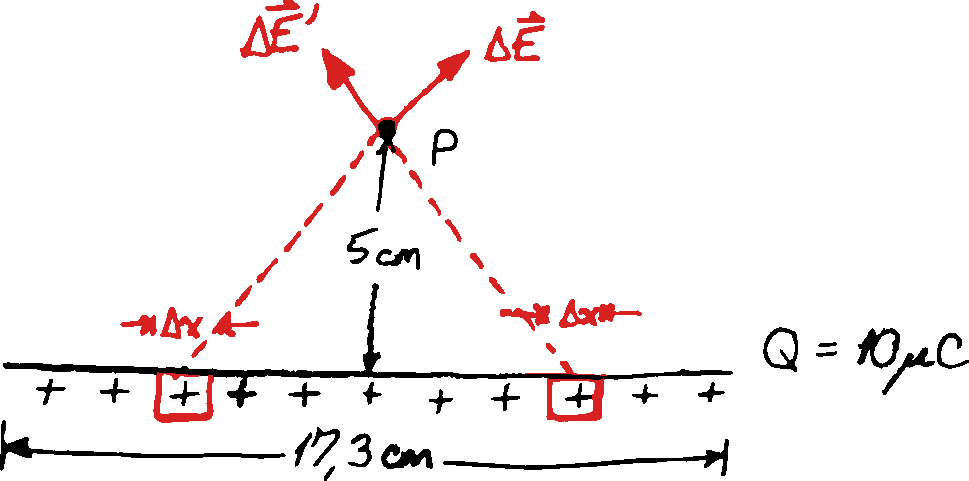
\includegraphics[scale=0.5]{02-champ-electrique/figures/champ-fil-3.pdf}
\end{center}


\textit{Solution. L'idée clé est que la composante horizontale du champ doit
  être nulle puisque les composantes horizontales des éléments de chaque côté
  du centre de la tige s'annulent deux à deux. La situation est illustrée
  ci-dessus.}

\paragraph{Partie 2 --- Champ produit par un élément de longueur}

À la lumière de la partie 1, trouver une expression pour la composante
verticale du champ électrique produit par un élément de longueur, i.e.: on
cherche une expression pour $dE_y$.

\begin{center}
  \begin{tikzpicture}
    \draw (-4, 0) -- (4, 0);
    \draw (-4, -0.1) -- (4, -0.1);
    \coordinate (P) at (0, 3);
    \coordinate (O) at (0, 0);
    \coordinate (l) at (-2, 0);
    \coordinate (r) at (2, 0);
    \node[anchor=west] (Pn) at (P) {$P$};
    \fill (P) circle(2pt);
    \draw[<->] (O) -- node[fill=white] {$D$} ($(P) - (0, 0.08)$);
    \fill ($(l) - (0.1, 0)$) rectangle ++(0.2, -0.1);
    \fill ($(r) + (0.1, 0)$) rectangle ++(-0.2, -0.1);
    \draw[dashed] (l) -- (P);
    \draw[dashed] (r) -- node[right] {$r$} (P);
    \draw[very thick,->] (P) -- ++({atan(3/2)}:1.5);
    \draw[very thick,->] (P) -- ++({180-atan(3/2)}:1.5);
    \draw ($(P) - (0, 0.5)$) arc (-90:{-atan(3/2}:0.5);
    \node at ($(P) + (0.2, -0.7)$) {$\theta$};
    \draw (0, -0.1) -- (0, -0.3) node[below] {$0$};
    \draw (r) -- ++(0, -0.3) node[below] {$x$};
    \draw[->] (-3.5, 1.5) -- (-2, 1.5) node[below] {$x$};
    \draw[->] (-3.5, 1.5) -- (-3.5, 3) node[left] {$y$};
  \end{tikzpicture}
\end{center}

  Un \textbf{élément de longueur} $d x$ produit un champ dont seule la
  composante verticale demeure (la composante horizontale étant annulée par
  celle d'un élément de longueur situé du côté opposé du fil.

  Pour trouver le champ électrique $dE_y$ produit, on fait l'approximation que
  l'élément de longueur est suffisamment petit pour qu'on puisse le considérer
  comme une charge ponctuelle. Le champ est donc

  $$d E_y = \frac{k d q}{r^2} \cos\theta.$$

  La charge est $dq = \lambda dx$ où $\lambda = Q / L$. La distance peut
  s'écrire

  $$d E_y = \frac{k \lambda dx}{r^2} \cos\theta.$$



\paragraph{Partie 3 --- Diminution du nombre de variables}

L'expression obtenue précédemment contient trois variables : $x$, $r$ et
$\theta$. Or, le fil est un objet à une dimension, il devrait donc être
possible d'exprimer l'élément de champ en terme d'une seule variable. Utiliser
la trigonométrie pour éliminer deux des trois variables.


On exprime tout en fonction de $\theta$. Il faut donc éliminer $x$ et $r$.

\begin{align*}
  \cos \theta &= \frac{D}{r} \\
           r  &= \frac{D}{\cos\theta}
\end{align*}

\begin{align*}
  \tan \theta &= \frac{x}{D} \\
           x  &= D\tan\theta \\
          dx  &= D\sec^2\theta d\theta
\end{align*}

Donc

  $$d E_y = \frac{k \lambda D\sec^2\theta d\theta}{D^2 / \cos^2\theta} \cos\theta.$$

qui se simplifie considérablement

  $$d E_y = \frac{k \lambda d\theta}{D} \cos\theta.$$



\paragraph{Partie 4 --- Application du principe de superposition}

Nous avons déterminé la composante verticale du champ produit par un élément de
longueur $dx$. Reste à déterminer la composante verticale du champ électrique
total au point $P$. Pour ce faire, nous n'avons qu'à intégrer l'expression que
nous avons obtenue sur toute la longueur de la tige. En faisant cela, nous
appliquons le principe de superposition.

\begin{align*}
  E_y &= \int_{\theta_1}^{\theta_2} \frac{k \lambda d\theta}{D} \cos\theta \\
      &= \frac{k \lambda}{D} \left[\sin\theta\right]_{\theta_1}^{\theta_2} \\
      &= \frac{k \lambda}{D} \left(\sin \theta_2 - \sin \theta_1 \right) \\
\end{align*}

Cette expression se simplifie en remarquant que
\begin{align*}
  \sin \theta_1 &= -\frac{L/2}{\sqrt{L^2/4 + D^2}} \\
  \sin \theta_2 &= \frac{L/2}{\sqrt{L^2/4 + D^2}} \\
\end{align*}

Donc
\[
  E_y = \frac{k \lambda}{D}\frac{L}{\sqrt{L^2/4 + D^2}}
\]

D'où
$$\vec{E} = \frac{k \lambda}{D}\frac{L}{\sqrt{L^2/4 + D^2}}\yhat$$


\paragraph{Partie 5 --- Vérification des cas extrêmes}

C'est toujours une bonne idée de vérifier les cas extrêmes pour s'assurer que
l'expression obtenue est cohérente dans ces cas. Qu'arrive-t-il si nous sommes
très loin de la tige ($D \gg L$)? Qu'arrive-t-il si nous sommes très proche
($D \ll L$)?

Loin:
\[
  E_y = \frac{k Q}{D^2}
\]

Proche: $\theta_1 = -\pi/2$ et $\theta_2 = \pi/2$ donc la différence des sinus
est $2$ et le champ est
\[
  E_y = \frac{2k\lambda}{D}
\]


\subsection*{Champ électrique d'une plaque infinie}

\paragraph{Partie 1 --- Symétrie et orientation du champ}
\marginpar{5 minutes}

En utilisant la symétrie de la situation, déterminer la direction dans la
laquelle le champ électrique doit être orienté au point $P$.

\begin{center}
  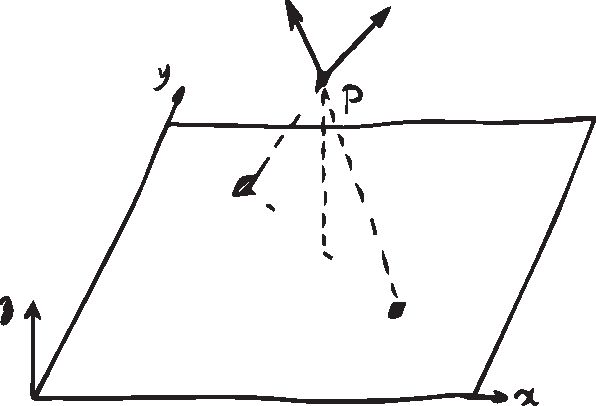
\includegraphics[scale=0.5]{02-champ-electrique/figures/champ-plaque-uniforme-1.pdf}
\end{center}


\textit{Solution. L'idée clé est que la composante horizontale du champ doit
  être nulle puisque les composantes horizontales des éléments de chaque côté
  du centre de la tige s'annulent deux à deux. La situation est illustrée
  ci-dessus.}

\paragraph{Partie 2 --- Champ produit par un élément de surface}

À la lumière de la partie 1, trouver une expression pour la composante
verticale du champ électrique produit par un élément de surface, i.e.: on
cherche une expression pour $dE_z$.

\begin{center}
  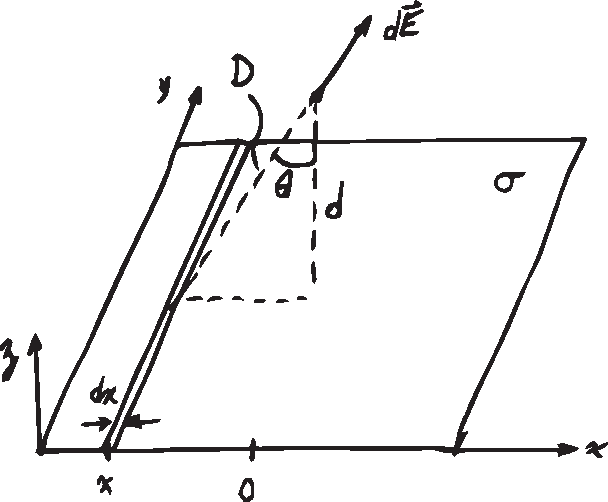
\includegraphics[scale=0.5]{02-champ-electrique/figures/champ-plaque-uniforme-2.pdf}
\end{center}

L'idée clé est de voir le plan chargé comme un ensemble de fils infinis collés
les uns aux autres. Chaque fil a une largeur $dx$ et produit un champ dont
seule la composante verticale demeure (la composante horizontale étant annulée
par un fil situé du côté opposé du plan).

Pour trouver le champ électrique $dE_z$ produit, on fait l'approximation que
l'élément de longueur est suffisamment petit pour qu'on puisse le considérer
comme un fil. Le champ est donc

$$d E_z = \frac{2k \lambda}{D} \cos\theta.$$

La densité de charge linéique du fil est donnée par la densité de charge
surfacique de la plaque multipliée par la largeur du fil

$$\lambda = \sigma dx.$$

La champ est donc

$$d E_z = \frac{2k \sigma dx}{D} \cos\theta.$$



\paragraph{Partie 3 --- Diminution du nombre de variables}

L'expression obtenue précédemment contient trois variables : $x$, $D$ et
$\theta$. Or, on peut construire le plan en collant des fils le long d'un seul
axe donc il est possible de tout exprimer en terme d'une seule variable. Utiliser
la trigonométrie pour éliminer deux des trois variables.


On exprime tout en fonction de $\theta$. Il faut donc éliminer $x$ et $D$.

\begin{align*}
  \cos \theta &= \frac{d}{D} \\
           D  &= \frac{d}{\cos\theta}
\end{align*}

\begin{align*}
  \tan \theta &= \frac{x}{d} \\
           x  &= d\tan\theta \\
          dx  &= d\sec^2\theta d\theta
\end{align*}

Donc

  $$d E_z = \frac{2k \sigma d\sec^2\theta d\theta}{d / \cos\theta} \cos\theta.$$

qui se simplifie considérablement

  $$d E_z = 2k \sigma d\theta.$$



\paragraph{Partie 4 --- Application du principe de superposition}

Nous avons déterminé la composante verticale du champ produit par un élément de
surface. Reste à déterminer la composante verticale du champ électrique
total au point $P$. Pour ce faire, nous n'avons qu'à intégrer l'expression que
nous avons obtenue sur toute la largeur de la plaque. En faisant cela, nous
appliquons le principe de superposition.

\begin{align*}
  E_z &= \int_{\theta_1}^{\theta_2} 2k \sigma d\theta \\
      &= 2k \sigma \left[\theta\right]_{\theta_1}^{\theta_2} \\
      &= 2k \sigma \left(\theta_2 - \theta_1 \right) \\
\end{align*}

Pour couvrir la plaque complètement, on doit prendre $\theta_1 = -\pi/2$ et
$\theta_2 = \pi/2$.

Donc
\begin{align*}
  E_z &= 2k \sigma \pi \\
      &= \frac{2 \sigma \pi}{4\pi\varepsilon_0} \\
      &= \frac{\sigma}{2\varepsilon_0}
\end{align*}

D'où
$$\vec{E} = \frac{\sigma}{2\varepsilon_0} \zhat$$


\paragraph{Partie 5 --- Vérification des cas extrêmes}

C'est toujours une bonne idée de vérifier les cas extrêmes pour s'assurer que
l'expression obtenue est cohérente dans ces cas. Qu'arrive-t-il si nous sommes
très loin de la plaque? Qu'arrive-t-il si nous sommes très proche?

Le résultat que nous avons obtenu est surprenant en ce sens qu'il ne dépend pas
de la distance du plan. Évidemment, un plan infiniment grand n'existe pas. Par
conséquent, le résultat n'est valable que pour un plan très grand duquel on est
suffisamment proche.


\subsection*{Champ électrique d'un arc de cercle chargé}

On considère un arc de cercle de rayon $R$ qui couvre un angle $\alpha$ et
porte une densité de charge linéique $\lambda$.  Quel est le champ électrique
au centre du cercle?

\begin{center}
  \begin{tikzpicture}
    \draw[decorate, decoration={
      markings, mark=between positions 0.1 and 1 step 6mm with {
        \node (0, 0) {$+$};
    }}] (-40:2.5) arc (-40:40:2.5);
    \draw (-40:2.7) arc (-40:40:2.7);
    \draw (-40:2.3) arc (-40:40:2.3);
    \draw[fill=black] (0, 0) circle (1pt);
    \draw (0, 0) -- node[fill=white] {$R$} ++(40:2.3);
    \draw (0, 0) -- ++(-40:2.3);
    \draw (-40:0.3) arc (-40:40:0.3);
    \draw[dashed, <-] (-1, 0) node[below] {$x$} -- (3, 0);
    \draw[fill=black!20] (-30:2.3) -- (-30:2.7) arc (-30:-25:2.7) -- (-25:2.3) -- cycle;
    \draw[dashed] (-27.5:2.3) -- (0, 0);
    \draw[ultra thick, ->] (0, 0) -- (152.5:2) node[above] {$d\vec{E}$};
    \draw (0:1) arc (0:-27.5:1);
    \draw[->|] (-34:2.8) -- (-30:2.8);
    \draw[->|] (-21:2.8) -- (-25:2.8);
    \node at (-27:3.2) {$Rd\theta$};
    \node at (-14:1.3) {$\theta$};
    \node[fill=white] at (0:0.6) {$\alpha$};
  \end{tikzpicture}
\end{center}

On prend un axe $x$ qui passe par le centre du cercle et le centre de l'arc.
Par symétrie, le champ électrique au centre n'aura qu'une composante le long de
l'axe $x$.

Un élément de longueur qui couvre un angle $\dif \theta$ à un angle $\theta$ a
une longueur $R\ddif \theta$ et porte une charge $\dif q = \lambda R \ddif
\theta$. La composante $x$ du champ créé par cet élément de longueur est
\[
  \dif E_x =  \frac{k\lambda R \ddif \theta}{R^2} \cos \theta
\]
Le champ total s'obtient en intégrant l'expression ci-dessus entre
$-\alpha / 2$ et $\alpha / 2$.
\begin{align*}
  E_x &= \int_{-\alpha / 2}^{\alpha / 2}
          \frac{k\lambda R \cos \theta}{R^2} \ddif \theta \\
      &=  \frac{k\lambda}{R} \int_{-\alpha / 2}^{\alpha / 2}
          \cos \theta \ddif \theta \\
      &= \frac{2k\lambda}{R} \sin(\alpha / 2)
\end{align*}
où la dernière ligne découle du fait que $\sin(\alpha / 2) = -\sin(-\alpha
/ 2)$.  Le champ de l'arc est donc
\[
  \vec{E} = \frac{2k\lambda}{R} \sin(\alpha / 2) \xhat
\]

Dans le cas d'un cercle complet, $\alpha = 2\pi$ et le sinus donne zéro, ce qui
fait que le champ total est nul, comme il se doit.


%\subsection*{Le champ électrique d'un anneau chargé}

%Considérons un anneau de rayon $R$ portant une densité linéique de charge
%$\lambda$. À partir de l'exemple précédent, on peut conclure que le champ
%électrique au centre de l'anneau est nul. Quel est le champ électrique à une
%distance $d$ au-dessus du centre de l'anneau?

%\begin{center}
    %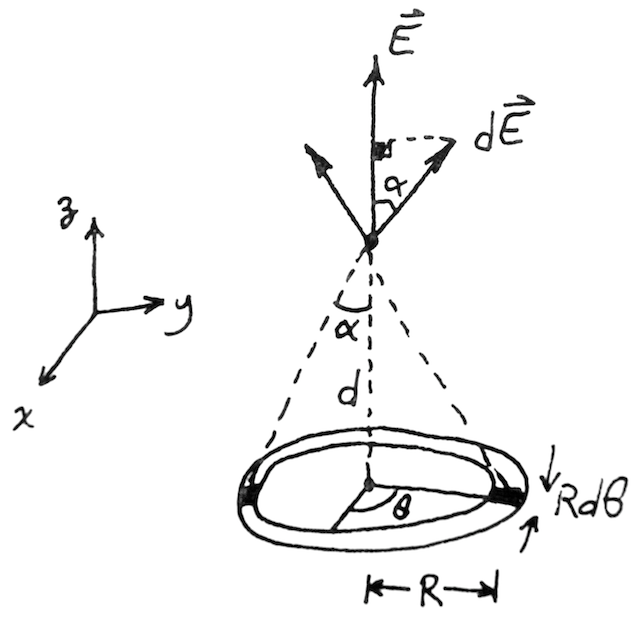
\includegraphics[scale=0.3]{02-champ-electrique/figures/ring.png}
%\end{center}

%Taking two identical line element on opposite sides of the ring show that the
%net electric field will point in the $z$ direction.  A line element spanning an
%angle $\dif \theta$ carries a charge $\lambda R \ddif \theta$.  The field in
%the $z$ direction due to that line element is
%\[
  %dE_z = \coulombcst \frac{\lambda R \cos \alpha \ddif \theta}{R^2 + d^2}
%\]
%and the net field is the integral around the ring.  Since the integrand does
%not depend on the position along the ring, the integral evaluates to just
%$2\pi$ hence
%\begin{align*}
  %E_z = \coulombcst \frac{2 \pi \lambda R \cos \alpha}{R^2 + d^2}
%\end{align*}
%Notice that the numerator is the circumference of the ring multiplied with the
%charge density.  This gives the total charge on the ring, $q$.  It is possible
%to get rid of the angle $\alpha$ using simple trigonometry.  One finds that
%\[
  %\cos \alpha = \frac{d}{\sqrt{R^2 + d^2}}
%\]
%The net field can be written as
%\[
  %\vec{E} = \coulombcst \frac{q d}{(R^2 + d^2)^{3/2}} \zhat
%\]


%\subsection{Electric Field of a Charged Disc}

%We now consider the electric field due to a disc of charge with surface charge
%density $\sigma$ and radius $R$.  The question is then to determine the field
%at a distance $d$ above the center of the disc (see Figure~\ref{fig:disc}).

%\begin{figure}
%\begin{center}
    %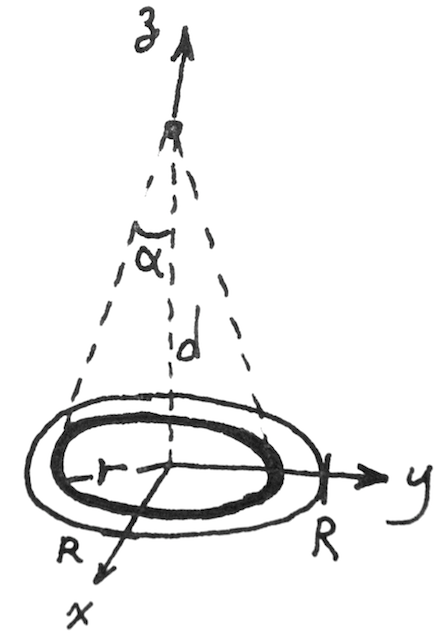
\includegraphics[scale=0.3]{02-champ-electrique/figures/disc.png}
%\end{center}
%\caption{A charged disc}
%\label{fig:disc}
%\end{figure}

%The disc can be considered as a collection of a large number of charged rings
%whose radius vary between $0$ and $R$.  A ring of radius $r$ and width $dr$
%carries a charge $dq = 2\pi r \sigma \,dr$.  The field it produces is then
%given by the equation obtained at the end of the previous example:
%\[
  %dE_z = \coulombcst \frac{2\pi r \sigma d\,dr}{(r^2 + d^2)^{3/2}}
%\]
%and the total field is obtained by integrating this expression.
%\begin{align*}
  %E_z = \frac{\sigma d}{2\varepsilon_0} \int_0^R \frac{r\,dr}{(r^2 + d^2)^{3/2}}
%\end{align*}
%This integral can be evaluated by the simple substitution $u = r^2 + d^2$:
%\begin{align*}
  %E_z &= \frac{\sigma d}{4\varepsilon_0} \int_{d^2}^{R^2 + d^2}
          %\frac{1}{2}\frac{du}{u^{3/2}} \\
      %&= \frac{\sigma d}{4 \varepsilon_0} \left[ \frac{u^{-1/2}}{-1/2}
          %\right]_{d^2}^{R^2 + d^2} \\
      %&= \frac{\sigma d}{2 \varepsilon_0} \left( \frac{1}{d} -
        %\frac{1}{\sqrt{R^2 + d^2}} \right) \\
      %&= \frac{\sigma}{2\varepsilon_0} \left( 1 - \frac{1}{\sqrt{(R/d)^2 + 1}}
        %\right)
%\end{align*}
%The electric field above the center of a disc is then
%\[
  %\vec{E} = \frac{\sigma}{2\varepsilon_0} \left( 1 - \frac{1}{\sqrt{(R/d)^2 + 1}}
        %\right) \zhat
%\]

%An interesting limit case is when the radius of the disc is much larger than
%the distance between the disc and the point at which the electric field is
%calculated.  Then, $R/d$ goes to infinity and the second term in the
%parenthesis goes to zero.  Hence the electric field at a distance $d$ from an
%infinite plane of charge is
%\[
  %\vec{E} = \frac{\sigma}{2\varepsilon_0} \zhat
%\]
%The strength of the field does not depend of the distance from the plane.


\sectionline


\section{Équilibre électrostatique}

\marginpar{Tremblay \S 2.9}

\paragraph{Objectif}

\begin{enumerate}
  \item L'étudiant comprendra ce qui se passe avec les charges dans un
    conducteur soumis à un champ électrique.
  \item L'étudiant saura comment déterminer le champ électrique dans un
    conducteur de même que dans une cavité à l'intérieur d'un conducteur.
\end{enumerate}


\subsection*{Le champ électrique à l'intérieur du conducteur est nul}

Preuve: s'il ne l'était pas, le champ électrique à l'intérieur exercerait une
force sur les électrons libres. Ils se déplaceraient dans la direction opposée
au champ électrique. On aurait alors une charge $+$ solitaire et une charge $-$
solitaire qui généreraient un champ électrique dans la direction opposée à
celle du champ initial. Le processus continuerait tant et aussi longtemps que
le champ électrique initial n'a pas été complètement neutralisé.



\subsection*{Le champ électrique à la surface d'un conducteur est toujours
  perpendiculaire à la surface}

Preuve: si ce n'était pas le cas, on aurait un mouvement des électrons libres
proches de la surface qui finirait par neutraliser la composante tangentielle
du champ.



\subsection*{Dans un conducteur chargé, toute la charge se retrouve à la surface
  extérieure}

Preuve: Le champ électrique à l'intérieur doit être nul. Si une charge nette
macroscopique se trouvait à l'intérieur, à proximiter de cette charge, le champ
électrique serait non-nul.



\subsection*{Dans une cavité à l'intérieur d'un conducteur, le champ électrique est
  nul}

On crée une cavité dans le conducteur. Tout le matériel enlevé est
neutre à cause du paragraphe précédent. Par conséquent, le matériel enlevé
n'exerçait aucune force sur les charges situées à la surface du conducteur.
Comme les charges à la surface étaient à l'équilibre avant d'enlever le
matériel, enlever du matériel qui n'exerçait aucune force ne changera pas leur
état d'équilibre.

Le champ électrique où le matériel a été enlevé était nul avant de faire le
trou. On a enlevé du matériel neutre qui ne contribuait donc pas au champ
électrique. Les charges qui étaient à la surface n'ont pas bougé (argument du
paragraphe précédent). Le champ électrique est déterminé complètement par la
configuration des charges. Par conséquent, le champ électrique dans la cavité
doit encore être nul.


\subsection*{Exercice avec des sphères métalliques}

Une charge $q = \si{4}{mC}$ dans une cavité au centre d'une sphère métallique.
Quelle est la charge sur la surface intérieur et la surface extérieur de la
sphère? Tracer les lignes de champ.


\subsection*{Champ d'un conducteur sphérique (ou isolant uniformément chargé)}

En réfléchissant aux lignes de champ, on peut voir que le champ à l'extérieur
d'une sphère métallique chargée est le même que si toute la charge était
concentré au centre.


\section{Champ électrique dans les diélectriques}

\marginpar{Tremblay \S 2.10}

\subsection*{Constante diélectrique}

\marginpar{5 minutes}

Le champ électrique induit dans un diélectrique est en général proportionnel au
champ électrique externe
$$\vE_\text{diel} = \alpha \vE_\text{vide}$$
donc le champ électrique total est
$$\vE = \vE_\text{vide} + \vE_\text{diel} = (1 + \alpha) \vE_\text{vide}.$$
On définit la \textbf{constante diélectrique} comme
$$\kappa = \frac{1}{1 + \alpha}$$
ie
$$\vE = \frac{1}{\kappa} \vE_\text{vide}.$$


\subsection*{Rigidité diélectrique}

Si le champ électrique externe appliqué sur un diélectrique est trop élevé, les
électrons seront arrachés aux atomes et un courant pourra traverser le
diélectrique. C'est ce qu'on appelle une \textbf{décharge}. Chaque matériau est
capable de supporter un champ électrique maximum qu'on appelle la
\textbf{rigidité diélectrique}.


%\chapter{Théorème de Gauss}


\section{Équilibre électrostatique}

\marginpar{Tremblay \S 2.9}

\paragraph{Objectif}

\begin{enumerate}
  \item L'étudiant comprendra ce qui se passe avec les charges dans un
    conducteur soumis à un champ électrique.
  \item L'étudiant saura comment déterminer le champ électrique dans un
    conducteur de même que dans une cavité à l'intérieur d'un conducteur.
\end{enumerate}


\subsection*{Le champ électrique à l'intérieur du conducteur est nul}

Preuve: s'il ne l'était pas, le champ électrique à l'intérieur exercerait une
force sur les électrons libres. Ils se déplaceraient dans la direction opposée
au champ électrique. On aurait alors une charge $+$ solitaire et une charge $-$
solitaire qui généreraient un champ électrique dans la direction opposée à
celle du champ initial. Le processus continuerait tant et aussi longtemps que
le champ électrique initial n'a pas été complètement neutralisé.



\subsection*{Le champ électrique à la surface d'un conducteur est toujours
  perpendiculaire à la surface}

Preuve: si ce n'était pas le cas, on aurait un mouvement des électrons libres
proches de la surface qui finirait par neutraliser la composante tangentielle
du champ.



\subsection*{Dans un conducteur chargé, toute la charge se retrouve à la surface
  extérieure}

Preuve: Le champ électrique à l'intérieur doit être nul. Si une charge nette
macroscopique se trouvait à l'intérieur, à proximiter de cette charge, le champ
électrique serait non-nul.



\subsection*{Dans une cavité à l'intérieur d'un conducteur, le champ électrique est
  nul}

On crée une cavité dans le conducteur. Tout le matériel enlevé est
neutre à cause du paragraphe précédent. Par conséquent, le matériel enlevé
n'exerçait aucune force sur les charges situées à la surface du conducteur.
Comme les charges à la surface étaient à l'équilibre avant d'enlever le
matériel, enlever du matériel qui n'exerçait aucune force ne changera pas leur
état d'équilibre.

Le champ électrique où le matériel a été enlevé était nul avant de faire le
trou. On a enlevé du matériel neutre qui ne contribuait donc pas au champ
électrique. Les charges qui étaient à la surface n'ont pas bougé (argument du
paragraphe précédent). Le champ électrique est déterminé complètement par la
configuration des charges. Par conséquent, le champ électrique dans la cavité
doit encore être nul.


\subsection*{Exercice avec des sphères métalliques}

Une charge $q = \si{4}{mC}$ dans une cavité au centre d'une sphère métallique.
Quelle est la charge sur la surface intérieur et la surface extérieur de la
sphère? Tracer les lignes de champ.


\subsection*{Champ d'un conducteur sphérique (ou isolant uniformément chargé)}

En réfléchissant aux lignes de champ, on peut voir que le champ à l'extérieur
d'une sphère métallique chargée est le même que si toute la charge était
concentré au centre.


\section{Champ électrique dans les diélectriques}

\marginpar{Tremblay \S 2.10}

\subsection*{Constante diélectrique}

\marginpar{5 minutes}

Le champ électrique induit dans un diélectrique est en général proportionnel au
champ électrique externe
$$\vE_\text{diel} = \alpha \vE_\text{vide}$$
donc le champ électrique total est
$$\vE = \vE_\text{vide} + \vE_\text{diel} = (1 + \alpha) \vE_\text{vide}.$$
On définit la \textbf{constante diélectrique} comme
$$\kappa = \frac{1}{1 + \alpha}$$
ie
$$\vE = \frac{1}{\kappa} \vE_\text{vide}.$$


\subsection*{Rigidité diélectrique}

Si le champ électrique externe appliqué sur un diélectrique est trop élevé, les
électrons seront arrachés aux atomes et un courant pourra traverser le
diélectrique. C'est ce qu'on appelle une \textbf{décharge}. Chaque matériau est
capable de supporter un champ électrique maximum qu'on appelle la
\textbf{rigidité diélectrique}.


%\chapter{Potentiel électrique}


\section{Énergie potentielle électrique}

\marginpar{Tremblay \S 4.1}

\paragraph{Objectif}

\begin{enumerate}
  \item L'étudiant pourra calculer le travail fait par une force électrique.
  \item L'étudiant saura comment démontrer que la force électrique est une
    force conservative.
  \item L'étudiant pourra calculer l'énergie potentielle électrique et sera en
    mesure d'expliquer le lien entre la force et l'énergie potentielle.
\end{enumerate}



\subsection*{Exercice de rappel sur la notion de travail}

\marginpar{Diapo}
\marginpar{10 minutes}

Classez les situations suivantes en ordre croissant du travail fait par la
force électrique sur la charge $q > 0$.

\begin{center}
  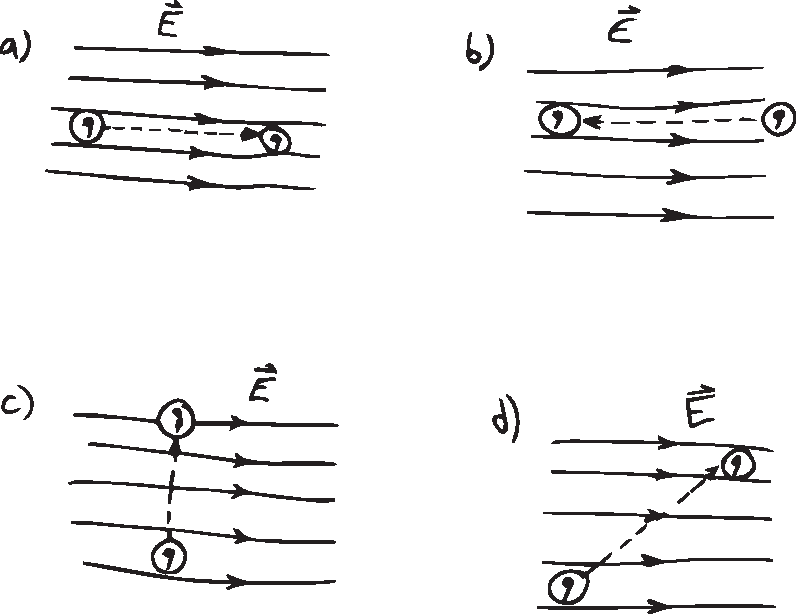
\includegraphics[scale=0.7]{04-potentiel/figures/travail-force-electrique.pdf}
\end{center}

\textit{Solution}: $W_b < W_c < W_a = W_d$


\subsection*{Le travail fait par une force électrique}

\marginpar{10 minutes}

On considère une région d'espace avec un champ électrique $\vec{E}$. Une charge
ponctuelle $q$ dans cette région subit une force électrique $\vec{F} =
q\vec{E}$. Si la particule se déplace du point $A$ au point $B$, le travail
effectué par la force électrique est
\[
  W = \int_A^B \vec{F} \cdot d\vec{s}
\]
où $d\vec{s}$ est une petite partie du chemin parcouru. Dans le cas simple où
la trajectoire est une ligne droite de longueur $L$ et le champ électrique est
uniforme
\[
  W = FL.
\]
On peut récrire l'expression du travail en terme du champ électrique
\[
  W = q \int_A^B \vec{E}\cdot d\vec{s}
\]
\begin{center}
  \begin{tikzpicture}
    \coordinate (A) at (0, 0);
    \coordinate (B) at (4, 2);
    \draw[fill=black] (A) circle (2pt);
    \draw[fill=black] (B) circle (2pt);
    \node[below] (nA) at (A) {$A$};
    \node[below] (nB) at (B) {$B$};
    \draw (A) -- plot[smooth] coordinates {(0.6, 0.8) (1.2, 1.5) (1.8, 1.2) (3.1, 2.5) (B)};
    \draw[ultra thick, ->] (1.8, 1.2) -- node[below] {$d\vec{s}$} (2.2, 1.58);
    \draw[ultra thick, ->] (1.8, 1.2) -- ++(0, 1.5) node[left] {$\vec{E}$};
  \end{tikzpicture}
\end{center}


\subsection*{Est-ce que la force électrique est conservative?}

\marginpar{Diapo}
\marginpar{15 minutes}

Une particule de déplace de l'origine $\vec{r}_0 = \vecxyz{0}{0}{0}$ jusqu'au
point $\vec{r} = \vecxyz{a}{b}{c}$ dans un champ électrique constant $\vec{E} =
E_z \zhat$ où $E_z$ est constant.  Déterminer le travail fait par la force
électrique pour les deux trajectoires suivantes.

\begin{itemize}
  \item Le long de la ligne droite qui relie $\vec{r}_0$ à $\vec{r}$.
  \item Le long de la ligne qui va de $\vec{r}_0$ à $\vecxyz{a}{b}{0}$, puis le
    long de la ligne qui va de $\vecxyz{a}{b}{0}$ à $\vecxyz{a}{b}{c}$.
\end{itemize}

\begin{description}
  \item[Le long de la ligne droite qui relie $(0,0,0)$ à $(a,b,c)$.]

    L'angle entre le champ électrique et le déplacement est constant sur toute
    la trajectoire :
    \[
      \cos \theta = \frac{c}{\sqrt{a^2 + b^2 + c^2}}.
    \]
    Le travail fait par la force électrique est donc
    \begin{align*}
      W &= \int_{(0,0,0)}^{(a,b,c)} E_z \cos \theta \, ds \\
        &= E_z \cos \theta \int_{(0,0,0)}^{(a,b,c)}\, ds \\
        &= E_z c,
    \end{align*}
    c'est-à-dire que le travail de la force électrique est déterminé par la
    composante du déplacement qui est parallèle au champ. Ceci ne devrait pas
    être une surprise.

  \item[Le long de la droite $(0,0,0)$ à $(a,b,0)$, puis le long de la droite
    $(a,b,0)$ à $(a,b,c)$.]

    Dans la première partie de la trajectoire, le déplacement est
    perpendiculaire au champ électrique, donc le travail effectué par la force
    électrique est nul. Pour la seconde partie de la trajectoire, le
    déplacement est parallèle au champ, le travail est donc  $E_z c$. Le
    travail total est donc encore $E_z c$.
\end{description}


\subsection*{Indépendance du chemin}

\marginpar{5 minutes}

L'exemple précédent suggère que le travail fait par la force électrique est
indépendant du chemin. Il est possible de montrer que c'est le cas, peu importe
le chemin choisi.

Une force pour laquelle le travail est indépendant du chemin est
\textbf{conservative}.

Rappelez-vous le cas de la force gravitationnelle à la surface de la Terre (ici
l'axe $y$ pointe vers le haut)
$$W_g = -mg \Delta y$$


\subsection*{Énergie potentielle électrique}

\marginpar{10 minutes}

Puisque la force électrique est conservative, on peut lui associer une énergie
potentielle. On définit l'énergie potentielle électrique de la même façon que
nous avons défini l'énergie potentielle gravitationnelle: c'est l'opposé du
travail fait par la force,
$$\Delta U = -W$$
ie,
\[
  \Delta U = - q\int_A^B \vec{E} \cdot d\vec{s}
\]


\subsection*{Exemple}

\marginpar{40 minutes}
\marginpar{Diapo}

On considère une mince tige métallique cylindrique très longue portant une
charge uniforme.  La densité linéique de charge est de $\lambda =
\SI{0.948}{\micro\coulomb\per\meter}$. Un électron est relâché \SI{35}{mm}
de la tige.

\begin{enumerate}
  \item Calculer la variation d'énergie potentielle du système après que
    l'électron se soit déplacé de \SI{1}{cm}.
  \item Si l'électron était initialement au repos, déterminer sa vitesse à la
    fin de son déplacement.
  \item Tracer un graphique du module du champ électrique généré par la tige en
    fonction de la distance par rapport à son axe.
  \item Tracer un graphique de l'énergie potentielle de l'électron en fonction
    de sa distance par rapport à l'axe de la tige.
\end{enumerate}

\paragraph{Solution}

\begin{center}
  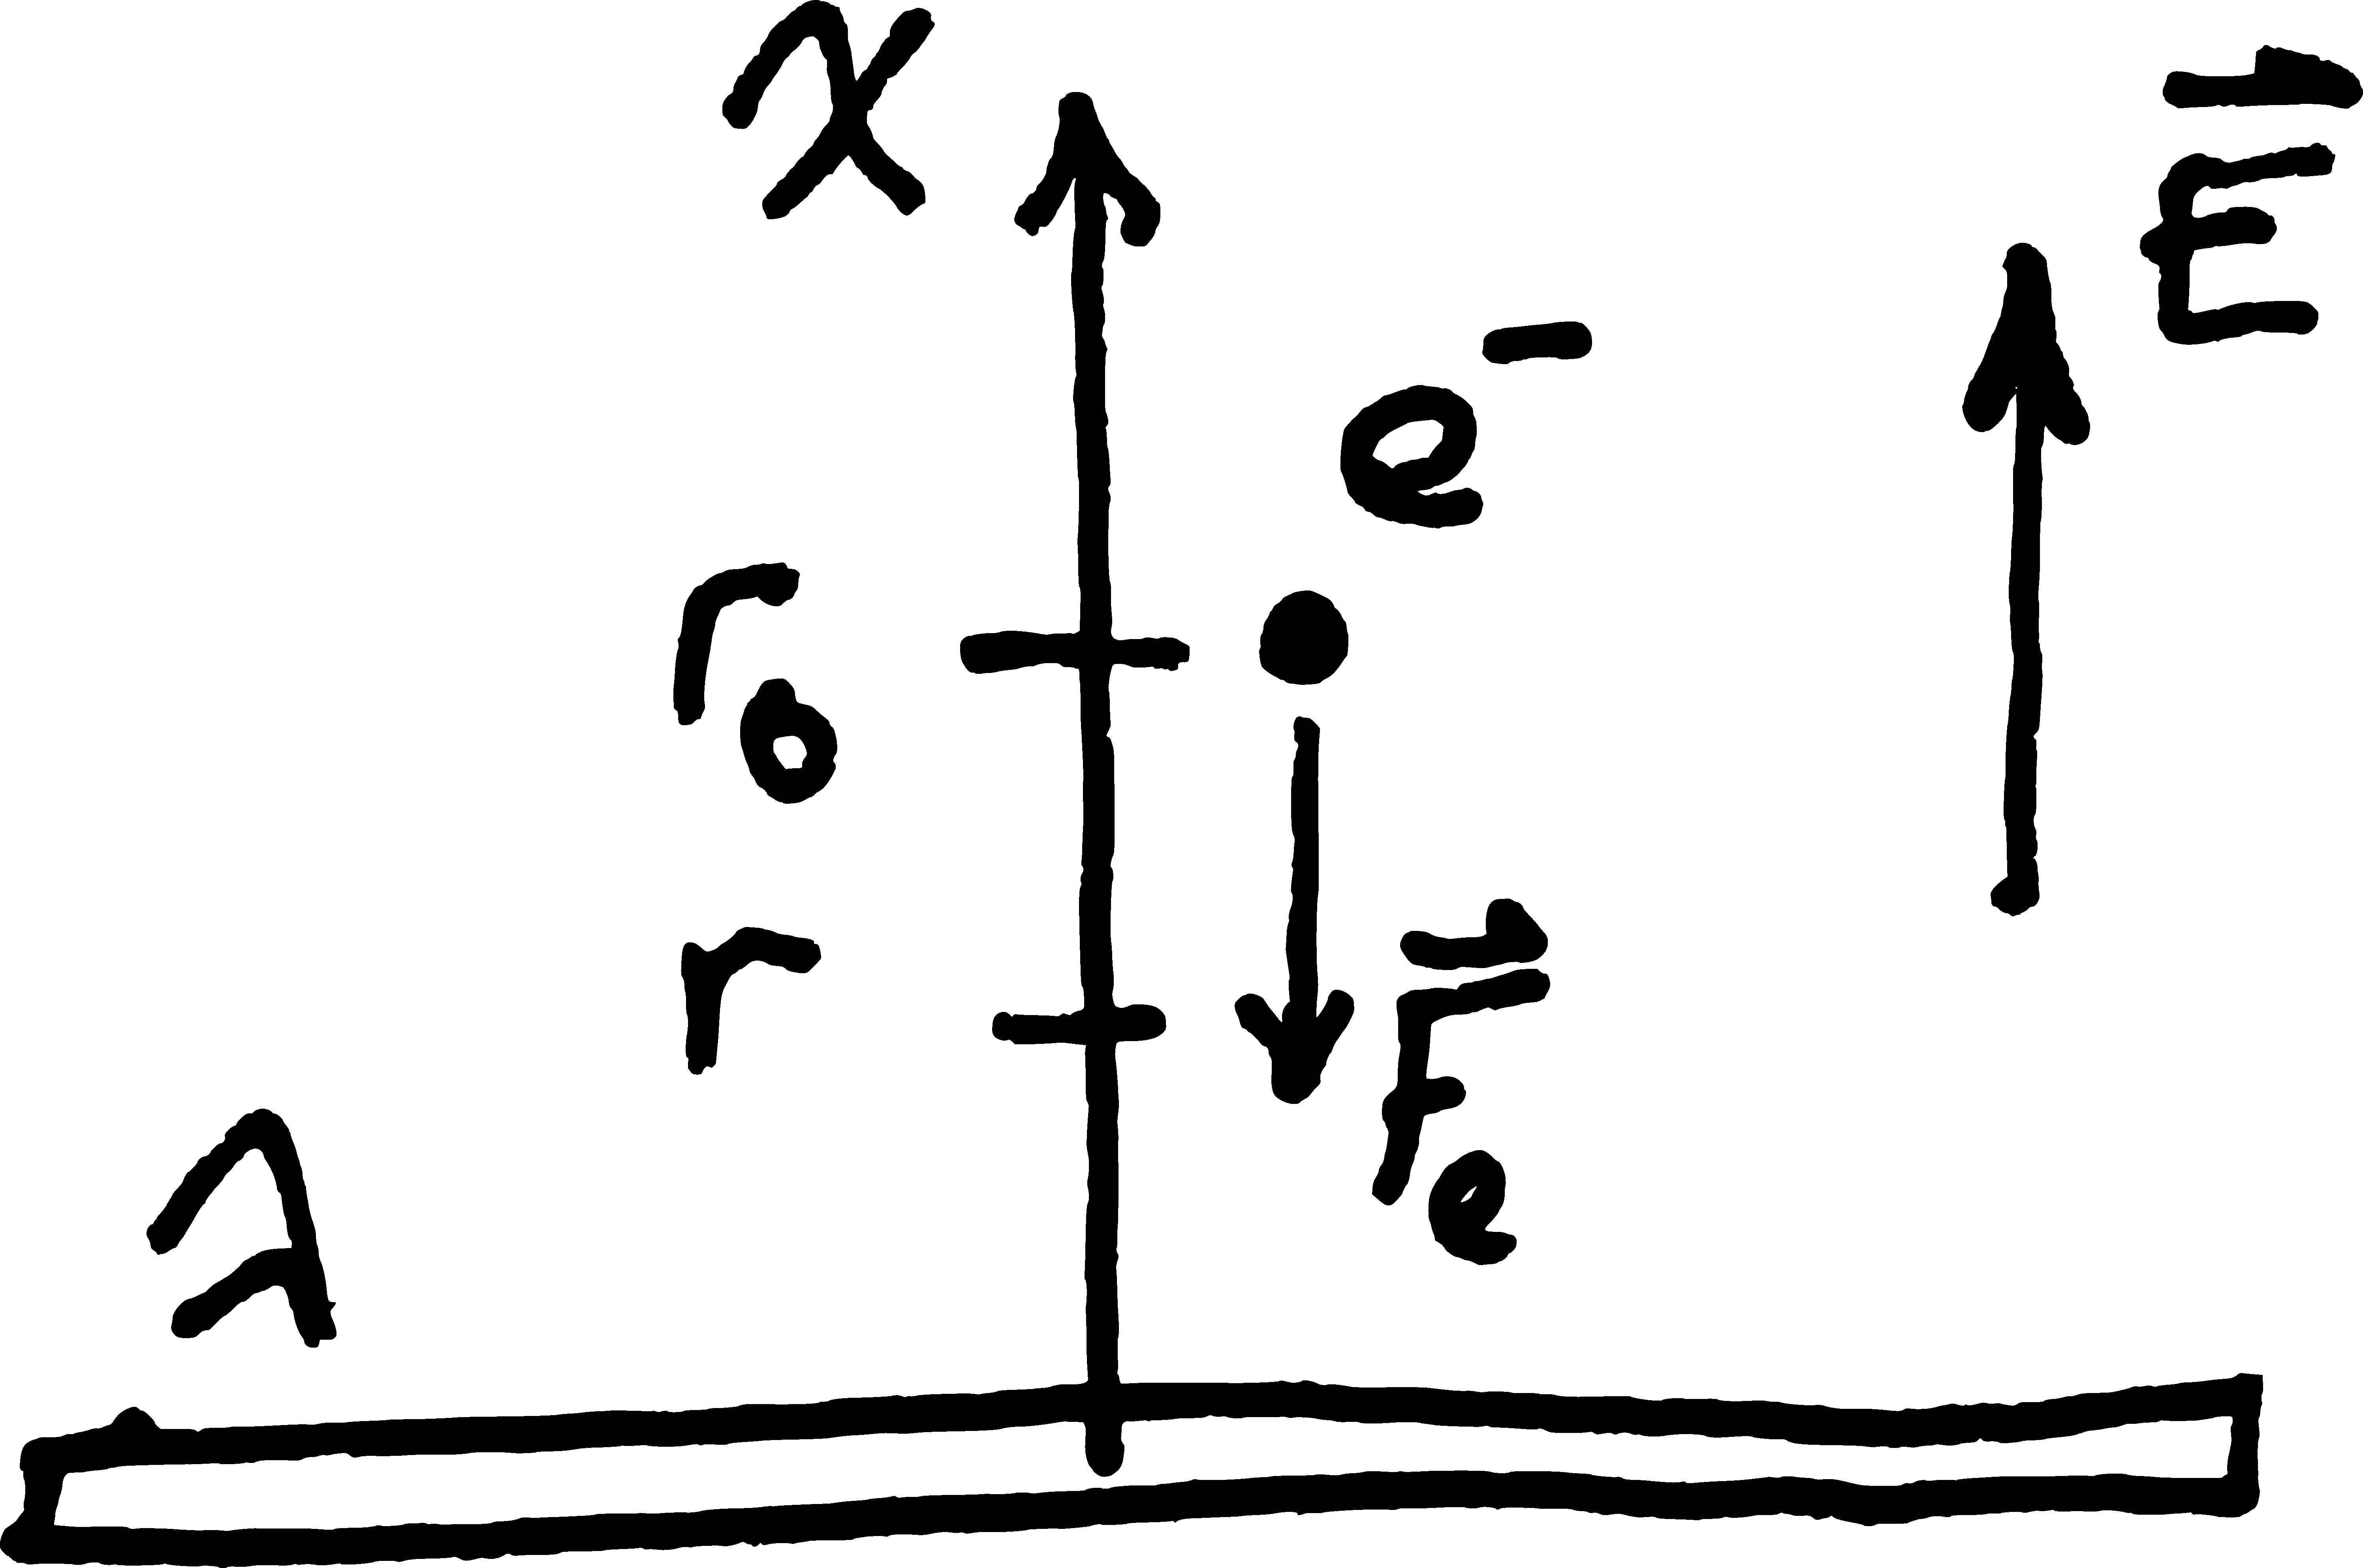
\includegraphics[scale=0.04]{04-potentiel/figures/exercice-tige-energie-potentielle.pdf}
\end{center}
\begin{enumerate}
    \item L'électron est attiré par la tige chargée positivement, donc il se
        rapproche de la tige. Le champ électrique de la tige est celui d'un fil
        infini soit
        \[\vE = \frac{2k\lambda}{x} \xhat.\]
        On peut donc calculer la différence d'énergie potentielle
        \begin{align*}
            \Delta U &= -q \int_{r_0}^{r} \frac{2k\lambda}{x} \xhat \cdot d\vec{s} \\
                     &= -2k\lambda q \int_{r_0}^r \frac{1}{x} \xhat \cdot (dx \xhat
                        + dy \yhat + dz \zhat) \\
                     &= -2k\lambda q \int_{r_0}^r \frac{1}{x} dx \\
                     &= -2k\lambda q \left[ \ln(r) - \ln(r_0) \right] \\
                     &= -2k\lambda q \ln\left( \frac{r}{r_0} \right) \\
                     &= 2k\lambda e  \ln\left( \frac{r}{r_0} \right) \\
                     &= \SI{-9.186e-16}{J}
        \end{align*}
    \item Au départ, son énergie cinétique était nulle car il était immobile,
        par conséquent
        \begin{align*}
            \Delta K = K_f - K_i = K_f.
        \end{align*}
        Par le principe de conservation de l'énergie mécanique
        \begin{align*}
            \Delta K + \Delta U &= 0 \\
            \Delta K &= -\Delta U \\
            \frac{1}{2} m_e v^2 &= -\Delta U \\
            v &= \sqrt{\frac{-2\Delta U}{m_e}} \\
            v &= \SI{4.491e7}{m/s}
        \end{align*}
        Donc
        \[\vec{v} = -\SI{4.491e7}{m/s} \xhat\]
    \item Les graphiques du module du champ magnétique et de l'énergie
        potentielle sont ci-dessous.

      \begin{center}
        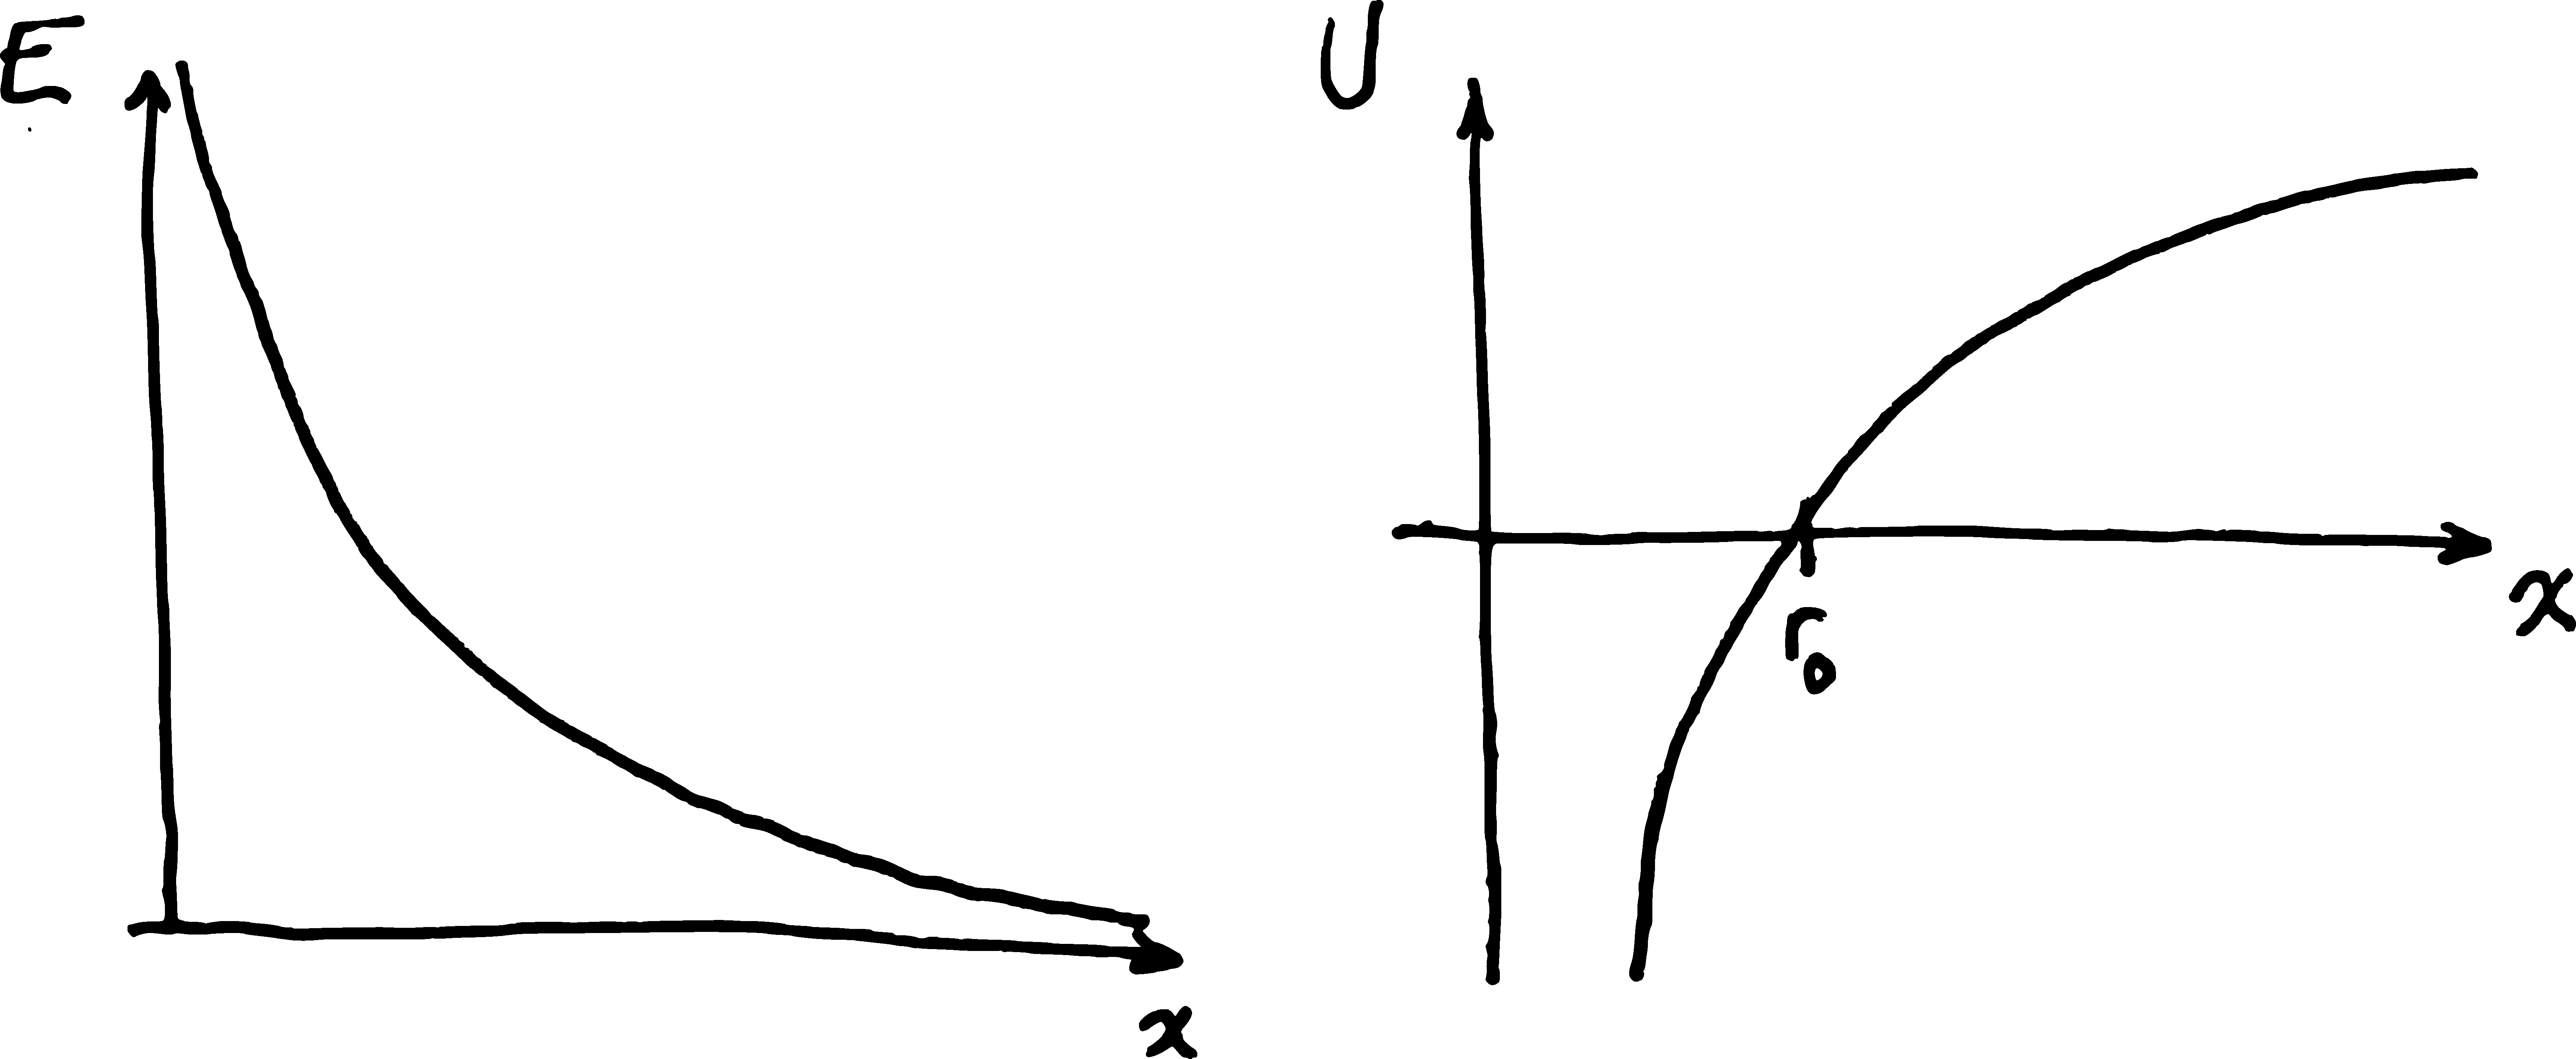
\includegraphics[scale=0.09]{04-potentiel/figures/exercice-tige-energie-potentielle-graphiques.pdf}
      \end{center}
\end{enumerate}


\sectionline


\section{Potentiel électrique}

\marginpar{Tremblay \S 4.2}

\paragraph{Objectif}

\begin{enumerate}
  \item L'étudiant comprendra les concepts de potentiel électrique et de
    différence de potentiel. Il pourra expliquer le lien entre le potentiel et
    le champ électrique.
\end{enumerate}



\subsection*{La différence de potentiel électrique}

\marginpar{10 minutes}

Dans la formule pour l'énergie potentielle électrique
\[
  \Delta U = -q \int_A^B \vec{E}\cdot d\vec{s},
\]
on remarque que l'intégrale ne dépend pas du tout de la charge qui se déplace.
L'intégrale dépend uniquement de la source du champ électrique. Comme nous
l'avions fait avec la force et le champ électrique, nous pouvons définir une
quantité qui ne dépend que de la source
\[
  \Delta V = - \int_A^B \vec{E}\cdot d\vec{s}.
\]
Cette quantité s'appelle une \textbf{différence de potentiel électrique}.

Les unités de la différence de potentiel sont les volts
$$\SI{1}{V} = \SI{1}{Nm/C}$$

On exprime souvent le champ électrique en \si{\volt\per\meter}.

Si une particule chargée $q$ se déplace entre deux points séparés par une
différence de potentiel $\Delta V$, sont énergie potentielle varie de
\[
  \Delta U = q \Delta V
\]


\subsection*{Exemple}

\marginpar{10 minutes}
\marginpar{Diapo}
Deux grandes plaques métalliques sont maintenues à une différence de potentiel
de \SI{12}{V}. Elles sont séparées d'une distance de \SI{1}{cm}. Un électron
qui se trouve juste à côté d'une des plaques se déplace jusqu'à l'autre plaque.
Si l'électron est initialement immobile, déterminer le module de sa vitesse
lorsqu'il atteint l'autre plaque.

\begin{center}
  \begin{tikzpicture}
    \draw[very thick] (0, 0) -- (0, 2);
    \draw[very thick] (4, 0) -- (4, 2);
    \foreach \y in {0.25, 0.75, ..., 1.9} {
      \node at (-0.3, \y) {$+$};
      \node at (4.3, \y) {$-$};
    }
    \fill (3.8, 1) circle (0.1);
    \node at (3.75, 0.6) {$e^{-}$};
    \draw[->] (3.65, 1) -- ++(-1, 0);
  \end{tikzpicture}
\end{center}

L'énergie cinétique initiale est de $0$ car l'électron est au repos. La
variation d'énergie potentielle lorsque l'électron passe de la plaque négative
à la plaque positive est de
\begin{align*}
  \Delta U &= q \Delta V \\
           &= -e \Delta V
\end{align*}
où $\Delta V = \SI{12}{V}$. Par le principe de conservation de l'énergie
mécanique, on a
\begin{align*}
  \Delta K + \Delta U &= 0  \\
      K_f - e\Delta V &= 0  \\
      K_f &= e\Delta V     \\
      K_f &= e \cdot \SI{12}{V}  \\
      K_f &= \SI{12}{eV}   \\
        v &= \sqrt{\frac{2 \cdot \SI{12}{eV}}{m}}  \\
        v &= \SI{2.055e6}{m/s}
\end{align*}


\subsection*{Électron-volt pour mesurer l'énergie}

\marginpar{5 minutes}

L'\textbf{électron-volt} (\si{eV}) est une unité de mesure d'énergie. Un
\si{eV} correspond à l'énergie cinétique que va acquérir un électron accéléré
dans une différence de potentiel de \SI{1}{V}.

\[
    \SI{1}{eV} = \SI{1.602e-19}{J}
\]


\subsection*{Exemple}

\marginpar{10 minutes}
\marginpar{Diapo}

Deux grandes plaques métalliques sont maintenues à une différence de potentiel
de \SI{12}{V}. On augmente la distance entre les plaques. Expliquez ce qui doit
se produire avec la densité surfacique de charge sur les plaques pour que la
différence de potentiel demeure constante.

\begin{center}
  \begin{tikzpicture}
    \draw[very thick] (0, 0) -- (0, 2);
    \draw[very thick] (4, 0) -- (4, 2);
    \node at (-0.5, 2.2) {$+\sigma$};
    \node at (4.5, 2.2) {$-\sigma$};
    \foreach \y in {0.25, 0.75, ..., 1.9} {
      \draw[->] (0.2, \y) -- (3.8, \y);
    }
    \node at (2, 1) {$\vE$};
    \draw[->] (-0.5, -0.5) -- (4.5, -0.5) node[below] {$x$};
  \end{tikzpicture}
\end{center}

Le champ généré par chaque plaque entre les plaques est
\begin{align*}
  E_{+} = \frac{\sigma}{2 \varepsilon_0} \quad\quad E_{-} = \frac{\sigma}{2 \varepsilon_0}
\end{align*}
donc le champ total entre les plaques est constant de grandeur
\[
  E = \frac{\sigma}{\epsilon_0}.
\]
Si on va d'un point $x_0$ à un point $x$, la différence de potentiel est
\begin{align*}
  \Delta V &= - \int_{x_0}^x \vE \cdot d\vec{s}  \\
           &= - \int_{x_0}^x E dx  \\
           &= - E\int_{x_0}^x dx  \\
           &= - E (x - x_0) \\
           &= - \frac{\sigma}{\varepsilon_0} (x - x_0) \\
\end{align*}
En particulier, si on va de la plaque négative à la plaque positive,
\[\Delta V = \frac{\sigma d}{\varepsilon_0} \]
donc, si la ddp est constante et que la distance entre les plaques augmente,
la densité surfacique de charge doit diminuer.



\subsection*{Potentiel électrique d'une charge ponctuelle}

Pour une charge ponctuelle
\[
  E_r = \coulombcst \frac{q}{r^2}.
\]
La différence de potentiel entre deux points $A$ et $B$ est donc
\begin{align*}
  \Delta V &= -\int_A^B \vec{E}\cdot d\vec{s} \\
    &= -\int_{r_A}^{r_B} \coulombcst \frac{q}{r^2} \,dr \\
    &= -kq \int_{r_A}^{r_B} \frac{1}{r^2} \,dr \\
    &= -kq \left[ \frac{-1}{r} \right]_{r_A}^{r_B} \\
    &= \frac{kq}{r_B} - \frac{kq}{r_A} \\
    &= V_B - V_A
\end{align*}
donc
$$V = \frac{kq}{r}$$


\sectionline


\subsection*{Travail personnel}

Faire les numéros 1, 2, 4, 10 et 22 du livre et les remettre avant de partir.


\sectionline


\subsection*{Rappels}

On a vu que le potentiel, l'énergie potentielle, la force et le champ
électrique sont reliés:

\begin{align*}
  \vF &= q\vE  \\
  \Delta U &= -\int_A^B \vF \cdot d\vec{s} = q \Delta V \\
  \Delta V &= -\int_A^B \vE \cdot d\vec{s} = \Delta U / q
\end{align*}

\begin{center}
\begin{tabular}{p{4cm}llp{4cm}}
  \toprule
  Objet    &     $\vE$      &   $V$     &  Notes  \\
  \midrule
  Charge ponctuelle $q$  &
      $\displaystyle{\frac{kq}{r^2} \vec{u}_r}$  &
      $\displaystyle{\frac{kq}{r}}$  &
      Potentiel nul à l'infini   \\[10pt]
  Tige infinie (au-dessus de l'axe)  &
      $\displaystyle{\frac{2k \lambda}{r}}\vec{u}_r$  &
      $\displaystyle{-2k \lambda \ln \left( \frac{r}{r_0} \right)}$  &
      Potentiel nul à la position initiale  \\[10pt]
  Plan infini  &
      $\displaystyle{\frac{\sigma}{2\varepsilon_0}\zhat}$  &
      $\displaystyle{\pm Ed}$  &
      Potentiel nul à la position initiale  \\[10pt]
  \bottomrule
\end{tabular}
\end{center}

Si on a une expression pour le potentiel, on peut facilement déterminer la
différence de potentiel entre deux points quelconques en calculant
\[\Delta V = V_f - V_i.\]



\subsection*{Exercice: potentiel d'une sphère conductrice}

Tracer le potentiel en fonction de la distance pour une sphère conductrice
chargée de rayon $R$ portant une charge $Q$.



\section{Potentiel d'un ensemble de charges}

\marginpar{Tremblay \S 4.3}

Le principe de superposition s'applique au potentiel électrique :
le potentiel d'un ensemble de charges est la somme des potentiels.

On peut utiliser ce principe pour calculer le potentiel de n'importe quel objet
chargé :
\[
  V = \int_\text{objet} \frac{k dq}{r}.
\]


%\subsection*{Potential of a Ring of Charge}

%Consider a charged ring or radius $R$ and total charge $q$.  Determine the
%electric potential a distance $d$ from the center of the ring on the axis
%perpendicular to the plane of the ring.

%There are two ways to proceed: use the potential of a point charge and
%integrate or use the electric field of a ring.

%\paragraph{With Potential of Point Charge}
%The ring can be thought of a collection of point charges.  Each line element
%of the ring produces a potential
%\[
  %dV = \coulombcst \frac{dq}{r}
%\]
%where $r = \sqrt{R^2 + d^2}$.  Since all line elements are at the same
%distance from the point at which we are calculating the potential, the
%integral over the ring is easily evaluated:
%\begin{align*}
  %V &= \int_\text{ring} \coulombcst \frac{dq}{r} \\
    %&= \coulombcst \frac{1}{r} \int_\text{ring} dq \\
    %&= \coulombcst \frac{q}{\sqrt{R^2 + d^2}}
%\end{align*}

%\paragraph{With Electric Field}
%If the $z$ axis is perpendicular to the plane of the ring and passes through
%the center of the ring, the electric field of the ring is
%\[
  %\vec{E} = \coulombcst \frac{qz}{(R^2 + z^2)^{3/2}} \zhat
%\]
%Consider the trajectory that goes from infinitely far on the $z$ axis down to
%$z = d$.  The potential is then
%\begin{align*}
  %V &= -\int_\infty^d \vec{E} \cdot (\zhat \,dz) \\
    %&= -\frac{q}{4\pi\varepsilon_0} \int_\infty^d \frac{z}{(R^2 + z^2)^{3/2}} \,dz \\
    %&= -\frac{q}{4\pi\varepsilon_0} \frac{1}{2} \int_\infty^{R^2 + d^2} \frac{1}{u^{3/2}} \,du \\
    %&= \frac{q}{4\pi\varepsilon_0} \left[\frac{1}{u^{1/2}}\right]_\infty^{R^2 + d^2} \\
    %&= \coulombcst \frac{q}{\sqrt{R^2 + d^2}}
%\end{align*}


%\subsection*{Exercice}

%Calculer le potentiel électrique à une distance $D$ au dessus d'un disque
%chargé de densité surfacique $\sigma$ et de rayon $R$.

%\begin{align*}
  %V &= \int_{0}^{R} \frac{k dq}{r} \\
    %&= \int_{0}^{R} \frac{k 2\pi a da}{\sqrt{a^2 + D^2}} \\
    %&= 2\pi k\sigma \left[ \sqrt{a^2 + D^2} \right]_0^R \\
    %&= 2\pi k\sigma \left[ \sqrt{R^2 + D^2} - D \right] \\
%\end{align*}



\subsection*{Énergie potentielle électrique d'un ensemble de charges}

On considère un ensemble de $n$ charges ponctuelles $q_1, q_2, \ldots, q_n$.
Pour calculer l'énergie potentielle de cet ensemble de charges, on doit
l'assembler, une charge à la fois. Placer la première charge ne requiert aucun
travail puisque le champ électrique est nul au départ. Apporter la seconde
charge nécessite un travail puisqu'on doit la déplacer dans le champ électrique
produit par la première charge. L'énergie requise est
\[
  U_2 = q_2 V_1.
\]
Pour la troisième charge, on doit tenir compte du potentiel créé par les deux
premières charges. Puisque le potentiel respecte le principe de superposition,
on a
\[
  U_3 = q_3 V_1 + q_3 V_2 = q_3 (V_1 + V_2).
\]
On peut répéter l'argument pour les charges suivantes. On obtient l'énergie
potentielle totale du système en additionnant les énergies $U_1, U_2, \ldots,
U_n$.  La somme contient un terme pour chaque paire de charges.
\[
  U = \sum_{i < j} q_i V_j
\]



\sectionline



\subsection*{Exercice}

Quatre charges sont placées aux sommets d'un carré de côté $d = \SI{3}{cm}$. Les
charges sont de $q_1 = \SI{1.7}{\micro\coulomb}$, $q_2 = \SI{-3}{\micro\coulomb}$,
$q_3 = \SI{5}{\micro\coulomb}$ et $q_4 = \SI{-4}{\micro\coulomb}$.


\begin{itemize}
  \item Déterminer le potentiel à \SI{2}{cm} en-dessous de la charge $q_1$.
  \item Déterminer l'énergie potentielle de cette distribution de charges.
\end{itemize}

\begin{center}
  \begin{tikzpicture}
    \coordinate (p1) at (0, 0);
    \coordinate (p2) at (2, 0);
    \coordinate (p3) at (2, 2);
    \coordinate (p4) at (0, 2);
    \node[draw, circle] (q1) at (p1) {$q_1$};
    \node[draw, circle] (q2) at (p2) {$q_2$};
    \node[draw, circle] (q3) at (p3) {$q_3$};
    \node[draw, circle] (q4) at (p4) {$q_4$};
    \draw[<->] (q1) -- node[fill=white] {$d$} (q2);
    \draw[<->] (q2) -- node[fill=white] {$d$} (q3);
    \draw[dashed] (q1) -- (q4);
    \draw[dashed] (q3) -- (q4);
  \end{tikzpicture}
\end{center}

\begin{align*}
  V &= V_1 + V_2 + V_3 + V_4 \\
    &= \frac{kq_1}{r_1} + \frac{kq_2}{r_2} + \frac{kq_3}{r_3} +
    \frac{kq_4}{r_4} \\
    &= \SI{67800}{V}
\end{align*}

\begin{align*}
  U &= q_1 V_2 + q_1 V_3 + q_1 V_4 + q_2 V_3 + q_2 V_4 + q_3 V_4 \\
    &= \frac{kq_1 q_2}{d} + \frac{kq_1 q_3}{\sqrt{2}d} + \frac{kq_1 q_4}{d} +
    \frac{kq_2 q_3}{d} + \frac{kq_2q_4}{\sqrt{2} d} + \frac{kq_3q_4}{d} \\
    &= \SI{-9.71}{J}
\end{align*}



\subsection*{Surfaces équipotentielles}

Une région connexe de l'espace qui est au même potentiel électrique est appelée
une \textbf{surface équipotentielle}. Par exemple, puisque le champ électrique
à l'intérieur d'un conducteur est nul, la surface d'un conducteur est une
équipotentielle.

Les surfaces équipotentielles sont toujours perpendiculaires aux lignes de
champ électrique. En effet, si on se déplace le long d'une équipotentielle,
$\Delta V = 0$. Or,
\[
  \Delta V = - \int \vE \cdot d\vec{s}
\]
n'est égal à zéro que si l'angle entre le déplacement et le champ électrique
est nul (en supposant que le champ électrique et le déplacement ne sont pas
nuls).



\subsection*{Exercice}

\marginpar{Diapo}

On place un électron dans une région de l'espace où les surfaces
équipotentielles sont telles qu'illustrées dans le schéma ci-dessous.

\begin{center}
  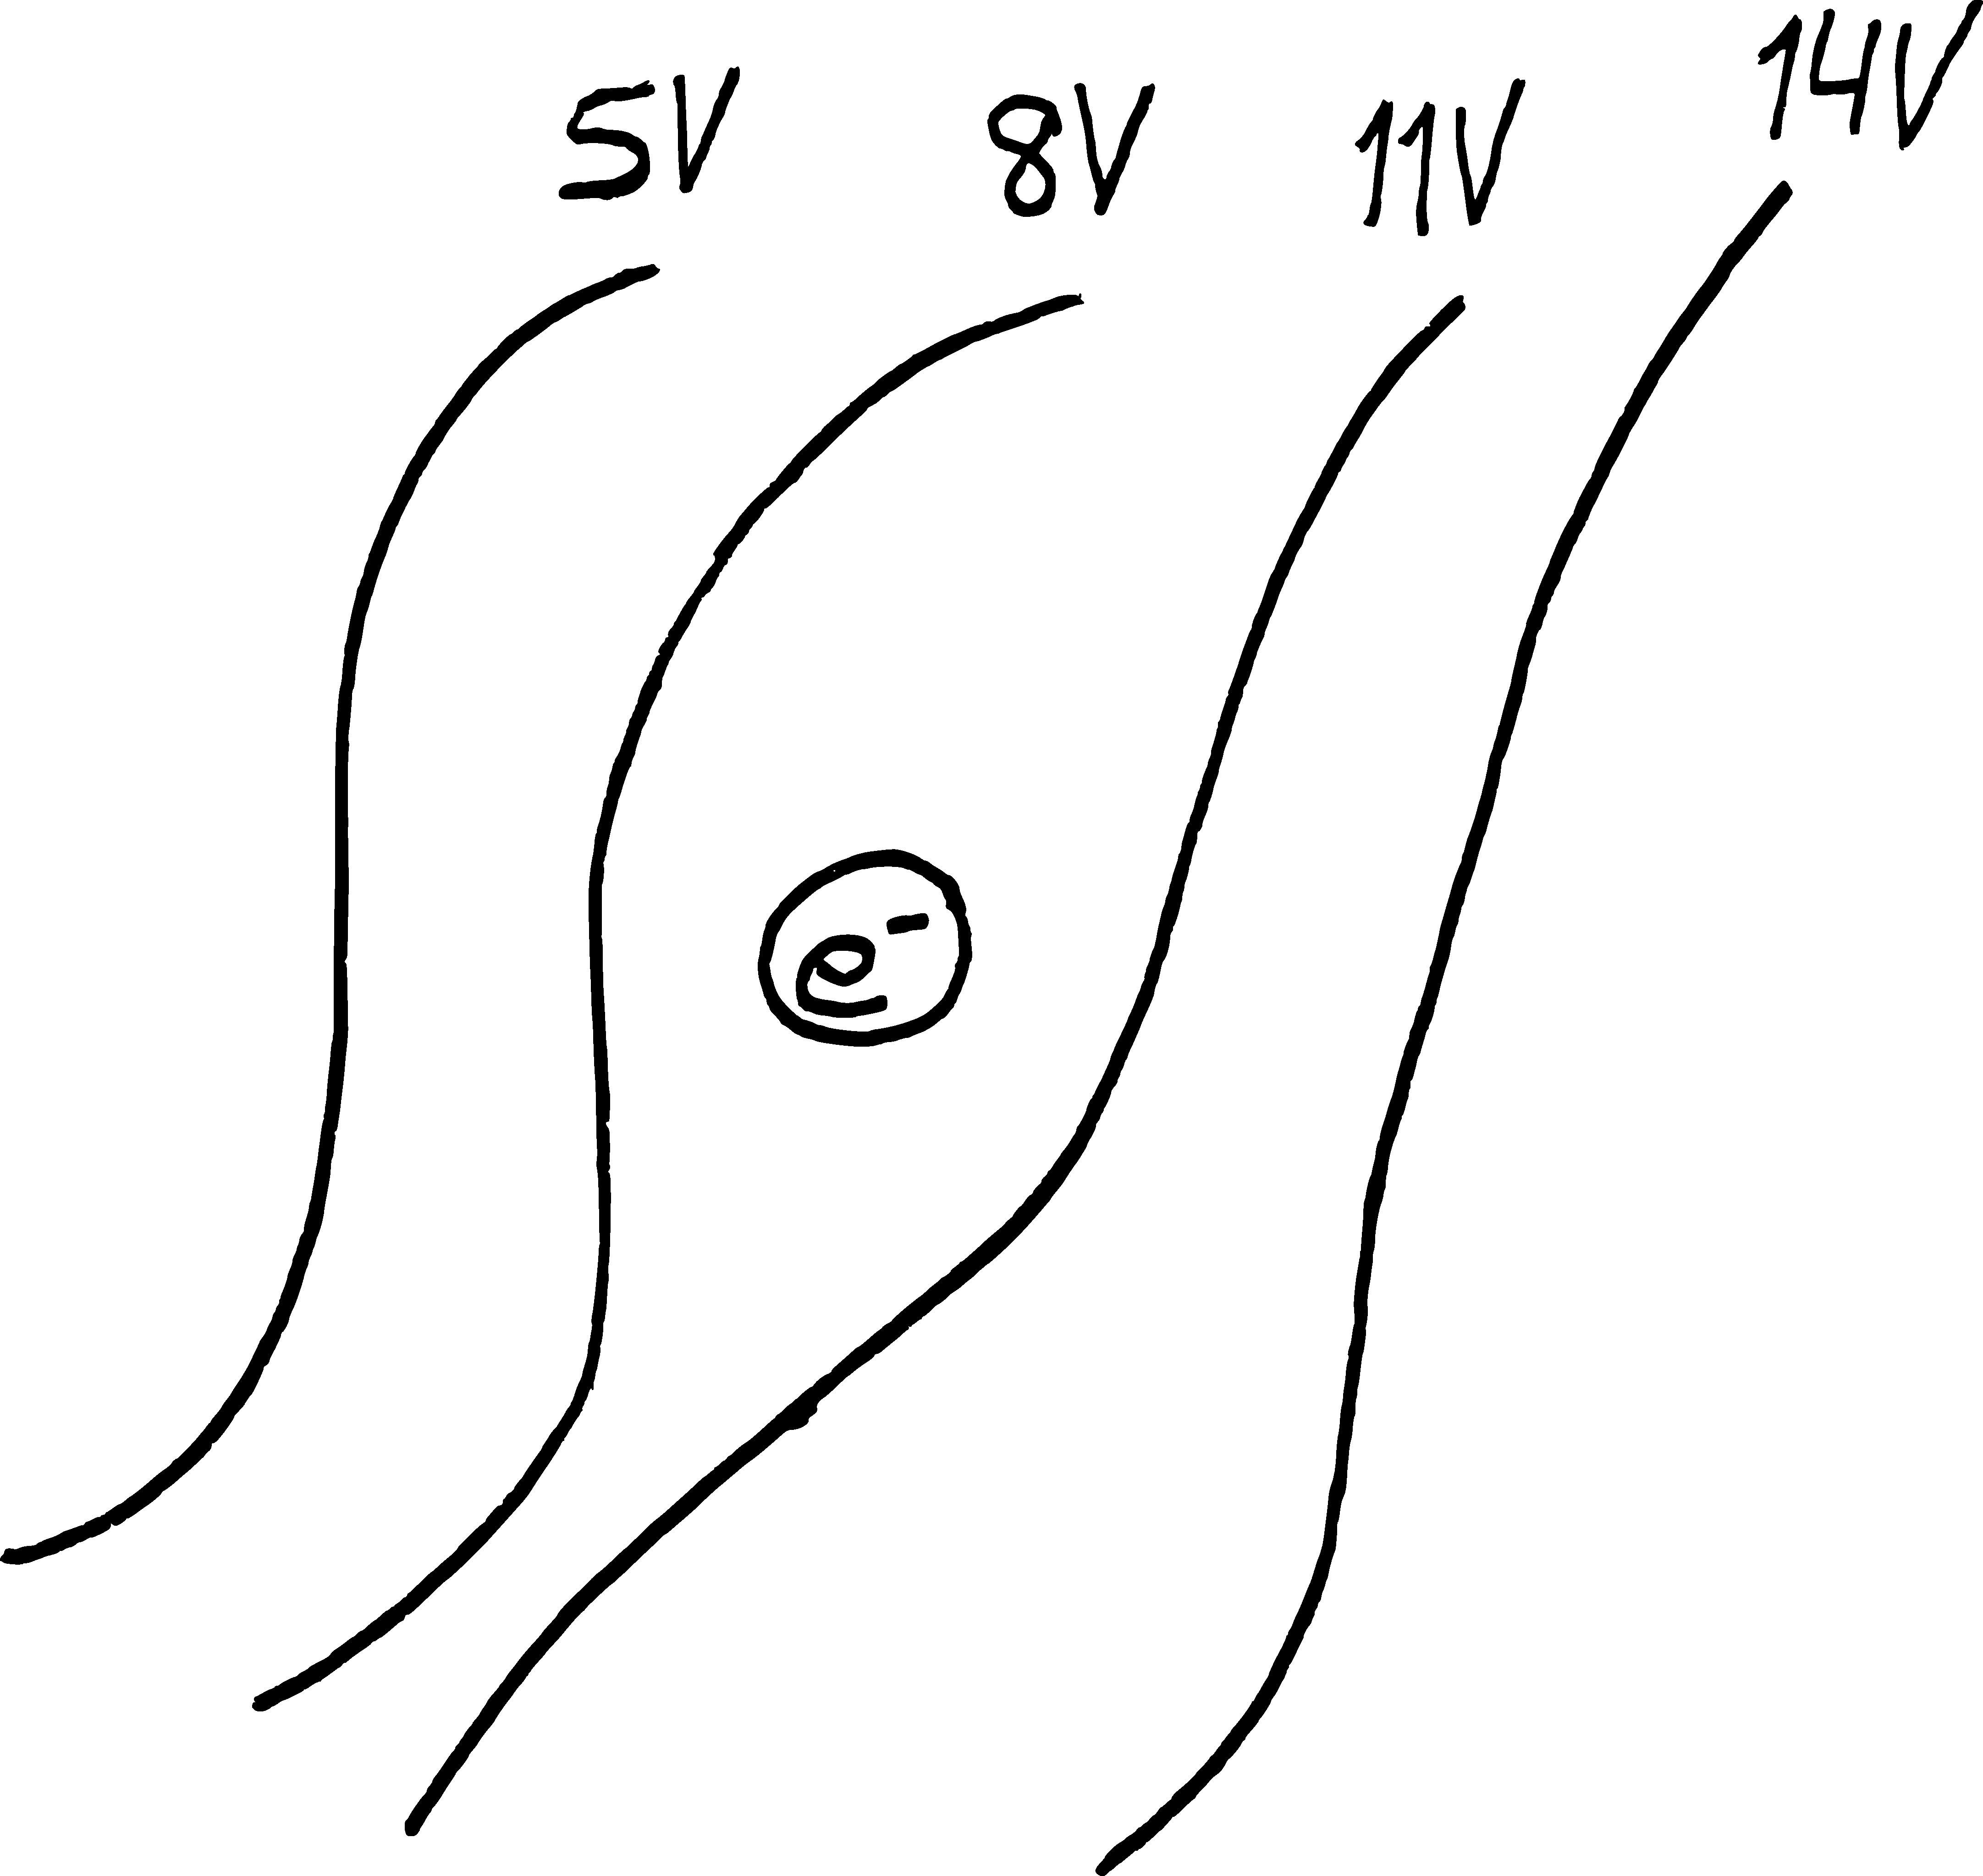
\includegraphics[width=5cm]{04-potentiel/figures/exercice-equipotentielles.pdf}
\end{center}

\begin{enumerate}
  \item Dans quelle direction est la force que subit l'électron?
  \item Tracez les lignes de champ électrique.
\end{enumerate}


\begin{center}
  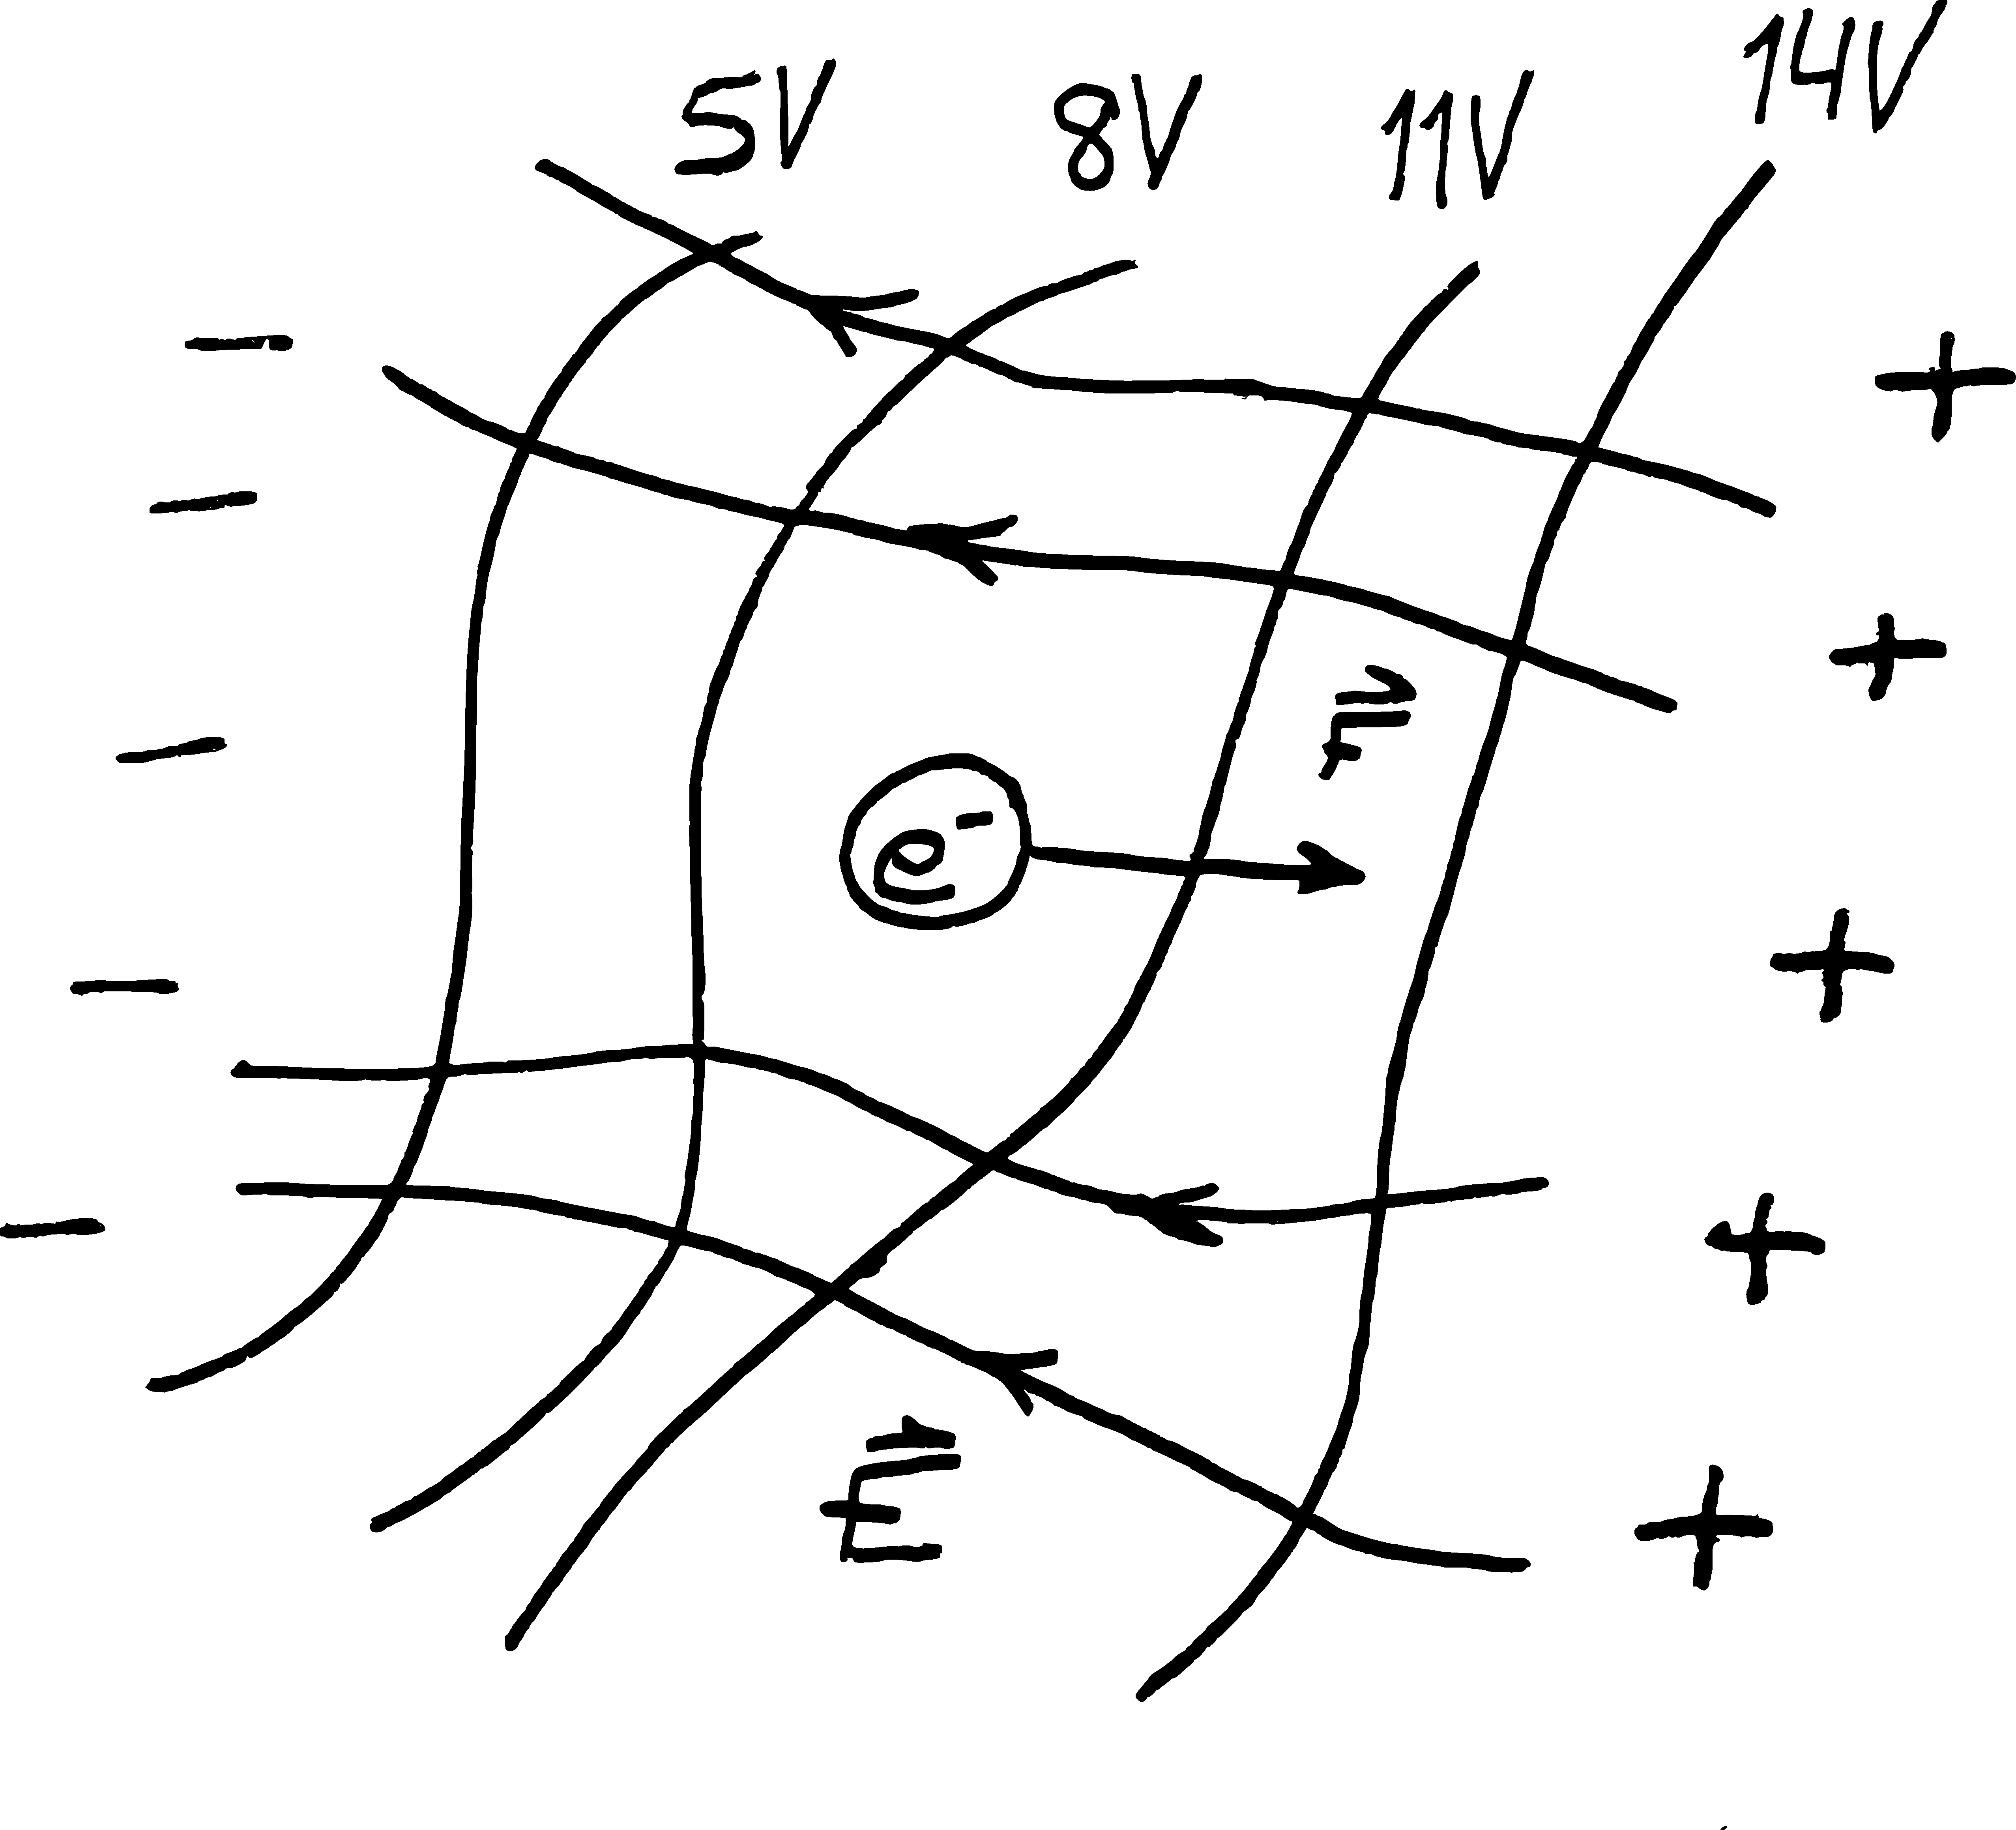
\includegraphics[width=5cm]{04-potentiel/figures/exercice-equipotentielles-solution.pdf}
\end{center}



Cet exercice permet de mettre en lumière quelques propriétés importantes des
équipotentielles et du potentiel électrique.

\begin{itemize}
  \item Plus les équipotentielles sont rapprochées les unes des autres, plus le
    champ électrique est grand à cet endroit.
  \item Les lignes de champ électrique vont des potentiels élevés vers les
    potentiels faibles.
  \item Une particule chargée négativement subira une force vers les potentiels
    élevés.
  \item Une particule chargée positivement subira une force vers les potentiels
    plus faibles.
\end{itemize}

%\chapter{Condensateurs}

\minisec{Objectif}

\begin{enumerate}
  \item L'étudiante saura ce qu'est un condensateur et comprendra le concept de
    capacité.
  \item L'étudiante sera en mesure de calculer la capacité de condensateurs dont
    la géométrie est simple.
  \item L'étudiante saura comment calculer l'énergie emmagasinée dans un
    condensateur.
  \item L'étudiante comprendra comment se comportent des condensateurs en série
    et en parallèle.
\end{enumerate}


\section{Condensateurs plans}

\marginnote{
  Tremblay \S 7.2

  Lafrance \S 5.2, 5.1
}

\begin{diapobox}
On considère deux grandes plaques parallèles connectées à une source de
tension.  Si on applique une différence de potentiel $\Delta V$ entre les deux
plaques, quelle charge sera emmagasinée sur chacune des plaques?

\begin{enumerate}
  \item Décrire le champ électrique entre les deux plaques.
  \item Déterminer le lien entre le champ électrique et la différence de
    potentiel.
  \item Montrer que la relation suivante est vraie
    $$Q = \frac{\epsilon_0 A}{d} \Delta V.$$
\end{enumerate}
\end{diapobox}


Un \textbf{condensateur} est constitué de deux \textbf{armatures} conductrices
portant des charges opposées séparées par un isolant. Dans un
\textbf{condensateur plan}, les armatures sont de très grandes plaques.

La \textbf{capacité} d'un condensateur décrit quelle charge peut être accumulée
sur l'armature positive pour chaque volt de différence de potentiel appliquée
entre les armatures. C'est une quantité qui ne dépend que de la géométrie du
condensateur et qui est reliée à la charge et à la différence de potentiel par
$$C = \frac{Q}{\Delta V}.$$

Dans le cas d'un condensateur plan
$$C = \frac{\epsilon_0 A}{d}.$$

Dans le système international, la capacité se mesure en farad (F). On note que
$$\SI{1}{\farad} = \SI{1}{\coulomb\per\volt}$$

\begin{center}
  \includegraphics[scale=0.5]{05-condensateurs/figures/condensateur-plan.pdf}
\end{center}


\minisec{Propriétés de condensateurs plans}

\begin{diapobox}
Lequel des énoncés suivants est vrai.

\begin{enumerate}
  \item Si l'aire des plaques augmente, la capacité diminue.
  \item La charge accumulée sur un condensateur plan augmente
    proportionnellement à la différence de potentiel entre les plaques.
  \item Si on augmente la distance entre les plaques, l'énergie potentielle du
    condensateur diminue.
\end{enumerate}


Lequel des énoncés suivants est vrai.

\begin{enumerate}
  \item Plus la distance entre les plaques est grande, plus la différence de
    potentiel doit être élevée pour maintenir la même charge sur les plaques.
  \item Si la densité surfacique de charge augmente et que la différence de
    potentiel demeure la même, c'est parce que la distance entre les plaques a
    diminué.
  \item Pour un condensateur donné, plus la différence de potentiel entre les
    plaques augmente, plus la capacité diminue.
\end{enumerate}

\end{diapobox}



\subsection{Condensateurs et diélectriques}

\marginnote{
  Tremblay \S 7.7
}

\paragraph{Objectif}

\begin{enumerate}
  \item L'étudiante connaîtra la définition de la constante diélectrique.
  \item L'étudiante comprendra comment l'introduction d'un diélectrique
    influence la capacité d'un condensateur.
\end{enumerate}

\marginnote{10 minutes}

Demander aux étudiants de résumer comment l'introduction d'un condensateur
entre les armatures d'un condensateur chargé affecte le champ électrique, la
différence de potentiel et la capacité.

Les éléments suivants devraient se retrouver dans la description.

\begin{itemize}
  \item Diélectrique se polarise ce qui crée un champ électrique dans le
    diélectrique dans la direction opposé au champ électrique causé par les
    armatures.
  \item Par le principe de superposition, le champ électrique total a un module
    inférieur à celui des armatures seules.
  \item La différence de potentiel diminue du même facteur puisqu'elle est
    proportionnelle au champ électrique.
  \item La charge sur les armatures est la même, mais la différence de
    potentielle est plus faible, donc la capacité a augmenté (car $C = Q/\Delta
    V$).
\end{itemize}


\minisec{Constante diélectrique}

\marginnote{5 minutes}

Le champ électrique induit dans un diélectrique est en général proportionnel au
champ électrique externe et en sens opposé
$$\vE_\text{diel} = -\alpha \vE_\text{vide}$$
donc le champ électrique total est
$$\vE = \vE_\text{vide} + \vE_\text{diel} = (1 - \alpha) \vE_\text{vide}.$$
On définit la \textbf{constante diélectrique} comme
$$\kappa = \frac{1}{1 - \alpha}$$
c'est-à-dire que
$$\vE = \frac{1}{\kappa} \vE_\text{vide}.$$
Par conséquent, la différence de potentiel entre les plaques chute d'un facteur
$\kappa$ et la capacité devient
$$C = \frac{Q}{\Delta V / \kappa} = \kappa C_\text{vide}.$$


\minisec{Rigidité diélectrique}

Si le champ électrique externe appliqué sur un diélectrique est trop élevé, les
électrons seront arrachés aux atomes et un courant pourra traverser le
diélectrique. C'est ce qu'on appelle un \textbf{claquage}. Chaque matériau est
capable de supporter un champ électrique maximum qu'on appelle la
\textbf{rigidité diélectrique}. Le tableau ci-dessous donne la rigidité
diélectrique de quelques matériaux.

\begin{diapobox}
  \begin{center}
  \begin{tabular}{lS}
    \toprule
    Substance       &        {Rigidité diélectrique (\si{V/cm})}     \\
    \midrule
    Air             &  30000  \\
    Verre           &  100000 \\
    Polystyrène     &  197000 \\
    Papier ciré     &  500000 \\
    Diamant         &  20000000 \\
    \bottomrule
  \end{tabular}
  \end{center}
\end{diapobox}


\section{Énergie dans un condensateur chargé}

\marginnote{
  Tremblay \S 7.5

  Lafrance \S 5.3
}

On doit construire la configuration de charge, ie, calculer le travail
nécessaire pour amener chacune des charges à sa place sur le condensateur.

Considérons un condensateur avec une capacité $C$ dont les armatures sont
maintenues à une différence de potentiel $\Delta V$.

La différence de potentiel lorsque la charge est $q$ est
$$\Delta V = \frac{q}{C}$$
donc l'énergie requise pour amener une charge supplémentaire $dq$ est
\begin{align*}
  dU &= dq \Delta V \\
           &= \frac{q}{C} dq
\end{align*}
L'énergie totale est la somme des variations d'énergie pour chacune des petites
charges nécessaires pour faire passer la charge totale du condensateur de $0$ à
$Q$:
\begin{align*}
  \Delta U &= \int_0^Q \frac{q}{C} dq \\
           &= \left. \frac{q^2}{2C} \right|_0^Q \\
           &= \frac{Q^2}{2C}
\end{align*}



\minisec{Condensateur qui explose}

Si on applique une différence de potentiel trop élevée aux armatures d'un
condensateur, le champ électrique entre les armatures deviendra plus grand que
la rigidité diélectrique du matériel isolant et on assistera à une décharge.
Très souvent, un condensateur qui subit une décharge explosera tel qu'illustré
dans le vidéo suivant \url{https://youtu.be/XBoaBwMRbnk?t=30}.


\begin{diapobox}
Dans un des cas, on voit un condensateur de \SI{470}{\micro\farad} qui explose.
Supposons qu'il a explosé à une tension de \SI{200}{\volt}. Quelle est la
quantité d'énergie qui peut être relâchée durant cette explosion?
\end{diapobox}

\begin{reponsebox}
\begin{align*}
  U &= \frac{C\Delta V^2}{2}  \\
    &= \SI{9.40}{J}
\end{align*}

C'est environ l'énergie d'un bloc de \SI{1}{kg} qui tombe d'une hauteur de
\SI{1}{m} sur le bout de votre doigt...
\end{reponsebox}



\section{Circuits simples avec des condensateurs}

\marginnote{Tremblay \S 7.4}

\subsection*{Condensateurs en série}

\marginnote{15 minutes}

Si plusieurs condensateurs sont placés en série, est-ce que la capacité de
l'ensemble est plus grande, plus petite ou égale à la somme des capacités?

La charge accumulée sur chacun des condensateurs est la même parce les
armatures opposées doivent avoir des charges opposées, et chaque section du
circuit doit être électriquement neutre.

\begin{center}
  \includegraphics[scale=0.5]{05-condensateurs/figures/condensateur-serie.pdf}
\end{center}

De plus, la somme des différences de potentiel aux armatures de chacun des
condensateurs doit être la même que la différence de potentiel fournie par la
source. On a donc
\begin{align*}
  \Delta V &= \Delta V_1 + \Delta V_2 + \Delta V_3  \\
  \frac{q}{C_\mathrm{eq}} &= \frac{q}{C_1} + \frac{q}{C_2} + \frac{q}{C_3}  \\
  \frac{1}{C_\mathrm{eq}} &= \frac{1}{C_1} + \frac{1}{C_2} + \frac{1}{C_3}
\end{align*}



\subsection*{Condensateurs en parallèle}

\marginnote{15 minutes}

Dans le cas de condensateurs en parallèle, la charge accumulée sur chaque
condensateur n'est pas nécessairement la même, mais la ddp aux bornes de chaque
condensateur elle doit être identique. La charge qui sera accumulée sur un
condensateur équivalent aux trois condensateurs doit être la somme des charges
sur chaque condensateur.

\begin{center}
  \includegraphics[scale=0.5]{05-condensateurs/figures/condensateur-parallele.pdf}
\end{center}

On a donc
\begin{align*}
  q &= q_1 + q_2 + q_3  \\
  C_\mathrm{eq} \Delta V &= C_1 \Delta V + C_2 \Delta V + C_3 \Delta V  \\
  C_\mathrm{eq} &= C_1 + C_2 + C_3
\end{align*}




\subsection*{Exemple}

On construit le circuit suivant avec une pile de \SI{9}{V}. Le condensateur 1 a
une capacité $C_1 = \SI{45}{\micro\farad}$ et ses armatures sont séparées par
du vide. Les condensateurs 2 et 3 sont construits exactement de la même façon que le
condensateur 1 sauf que tout l'espace entre leurs armatures est rempli par
du germanium et du papier, respectivement. La constante diélectrique du
germanium est 16 alors que celle du papier est 3.

\begin{center}
\begin{circuitikz}
  % French babel breaks everything... see https://latex.org/forum/viewtopic.php?t=11981
  \shorthandoff{:}\shorthandoff{!}
  \draw (0, 0) to[battery, l=$\SI{9}{\volt}$] (0, 3)
    to[C, l=$C_1$] (2, 3)
    to[C, l=$C_2$] (2, 0)
    to (0, 0);
  \draw (2, 3) to[short] (4, 3)
    to[C, l=$C_3$] (4, 0)
    to (2, 0);
\end{circuitikz}
\end{center}

\begin{enumerate}
  \item Déterminer la capacité équivalente à ces trois condensateurs.
  \item Déterminer la charge accumulée sur la plaque positive du condensateur 2.
  \item Déterminer l'énergie accumulée dans le condensateur 3.
\end{enumerate}


D'abord
\begin{align*}
  C_2 &= \kappa_\text{Ge} C_1 = 16C_1 = \SI{720}{\micro\farad} \\
  C_3 &= \kappa_\text{papier}C_1 = 3C_1 = \SI{135}{\micro\farad} \\
\end{align*}
$C_2$ et $C_3$ sont en parallèle donc
\begin{align*}
  C_{23} &= C_2 + C_3 \\
         &= \SI{855}{\micro\farad}
\end{align*}
$C_1$ est en série avec $C_{23}$ donc
\begin{align*}
  C_\text{eq} &= \frac{1}{\frac{1}{C_1} + \frac{1}{C_{23}}} \\
              &= \SI{42.8}{\micro\farad}
\end{align*}

La charge accumulée sur cette capacité équivalente serait la même que celle
accumulée sur $C_1$ et $C_{23}$. Donc
\begin{align*}
  Q_{23} &= C_\text{eq} \Delta V \\
         &= \SI{384.75}{\micro\coulomb}
\end{align*}
La différence de potentiel aux bornes de $C_2$ (et $C_3$) est donc
\begin{align*}
  \Delta V_{2} &= \frac{Q_{23}}{C_{23}} \\
               &= \SI{0.45}{\volt}
\end{align*}
d'où on peut déduire la charge accumulée sur $C_2$
\begin{align*}
  Q_2 &= C_2 \Delta V_2 \\
      &= \SI{324}{\micro\coulomb}
\end{align*}

L'énergie emmagasinée dans $C_3$ est obtenue par
\begin{align*}
  U_3 &= \frac{Q_3^2}{2C_3} = \frac{C_3 \Delta V_3^2}{2}  \\
      &= \SI{13.67}{\micro\joule}
\end{align*}




%\chapter{Courant électrique}

\section{Courant électrique}

\marginnote{
  Tremblay \S 5.1, 5.2

  Lafrance \S 6.1
}

\paragraph{Objectif}

\begin{enumerate}
  \item L'étudiant analysera un modèle de conduction impliquant la vitesse de
    dérive des électrons dans un conducteur.
\end{enumerate}


Le courant donne la quantité de charge par unité de temps qui traverse un fil
$$i_\mathrm{moy} \equiv \abs{\frac{\Delta Q}{\Delta t}}$$
En général, cette quantité peut fluctuer et la définition générale est
$$i \equiv \abs{\frac{dQ}{dt}}$$

La direction du courant est la direction des charges positives.


\subsection{Vitesse de dérive}

Regardons de plus près des électrons de conduction dans un fil.

Ils se déplacent dans des directions aléatoires. En première approximation, on
peut considérer les électrons de conduction comme formant un gaz parfait.
D'après le théorème d'équipartition en thermodynamique, l'énergie des électrons
est
$$\frac{3}{2} kT$$
ce qui permet de déterminer que leur vitesse thermique est de l'ordre de
\SI{1e5}{m\per s}.

Avec une différence de potentiel, les électrons se déplaceront légèrement plus
vers le potentiel le plus élevé. La vitesse thermique demeure et les collisions
aussi. Dans l'ensemble, la vitesse effective avec laquelle les électrons se
déplacent vers le potentiel positif est appelée la \textbf{vitesse de dérive}.
En général, la vitesse de dérive est de l'ordre de \SI{1e-6}{m\per s}.


\subsection{Courant et vitesse de dérive}

Considérons une section de fil de surface $A$. Dans un intervalle de temps
$dt$, seul les électrons qui se trouvent à une distance inférieure à $v_d
dt$ pourront traverser la section de fil. Combien d'électron de
conduction y a-t-il?
Supposons qu'il y en a $n$ par unité de volume dans le fil. La charge totale
qui peut traverser la surface est donc
\begin{align*}
  dQ = -env_ddt A
\end{align*}
d'où
\begin{align*}
  i = env_d A
\end{align*}

\begin{center}
  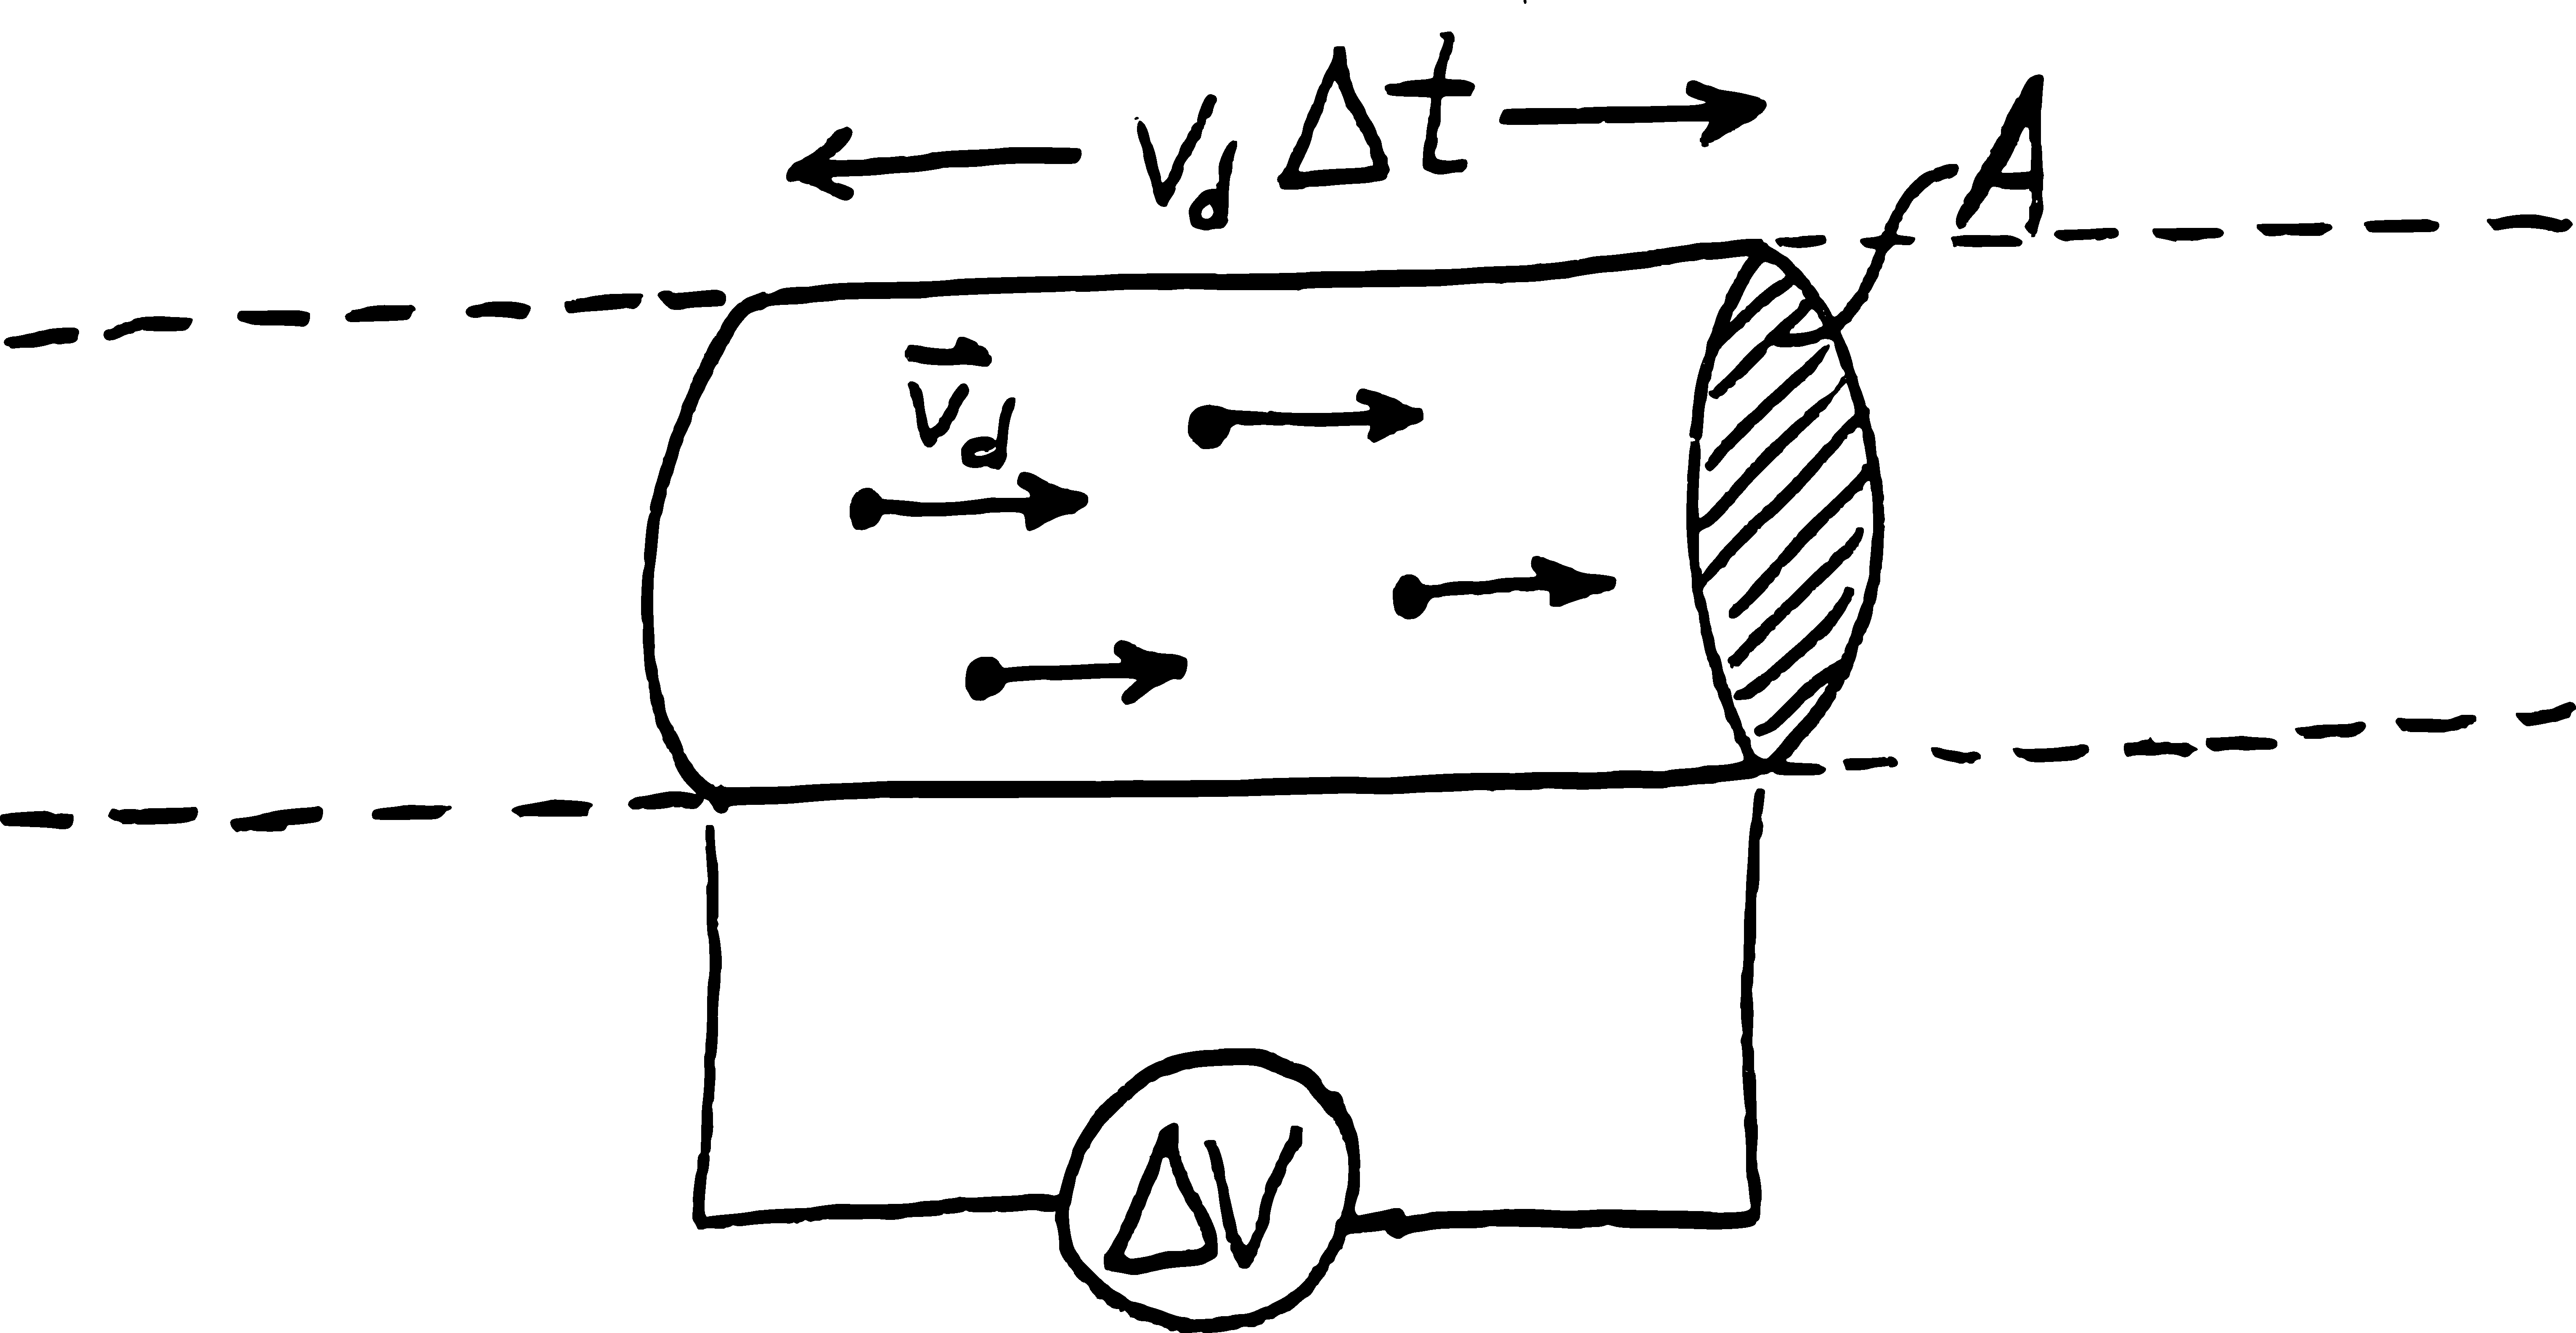
\includegraphics[width=5cm]{06-courant/figures/courant-vd.pdf}
\end{center}

On définit la \textbf{densité de courant} par
\begin{align*}
  J &\equiv \frac{i}{A} \\
    &= env_d
\end{align*}



\section{Modèle de conduction et résistance}

\marginnote{
  Tremblay \S 5.3

  Lafrance \S 6.2, 6.4, 6.5
}
Qu'en est-il de la vitesse de dérive? On se doute qu'elle dépend du champ
électrique, mais comment? D'abord, clarifions le fait qu'il existe un champ
électrique dans le fil même si c'est un conducteur. En effet, il y a des
charges qui bougent, donc la situation n'est pas à l'équilibre électrostatique.
Si le champ électrique est constant, on s'attend à ce que la force électrique
sur les charges en mouvement soit constante et donc que l'accélération des
charges soit constante. Si c'était le cas, on aurait une vitesse de dérive qui
augmente continuellement. Ce n'est pas ce qui est observé. On constate plutôt
que la vitesse de dérive est constante. Ceci est causé par les nombreuses
collisions que les charges en mouvement subissent lors de leur déplacement. Ces
collisions sont équivalentes à un mouvement dans un milieu résistant, comme une
voiture qui se déplace dans l'air. Si le milieu exerce une force
proportionnelle à la vitesse, on peut montrer que les charges atteindront une
vitesse limite constante. On a donc que
\[
  v_d = \mu_e E
\]
où $\mu_e$ est une constante de proportionnalité, la \textbf{mobilité} des
électrons. En combinant avec le résultat obtenu plus haut, on obtient la
relation suivante entre le courant et le champ électrique
\[
  i = en\mu_e AE.
\]
En terme de la densité de courant, on obtient
\[
  J = en\mu_e E.
\]
On définit la constante
\[
  \rho \equiv \frac{1}{en\mu_e}
\]
comme étant la \textbf{résistivité} du matériau.


Si on applique une différence de potentiel $\Delta V$ entre deux extrémités
d'un fil de longueur $l$ et de section $A$, le champ électrique est
$$E = \frac{\Delta V}{l}$$
donc la densité de courant est
$$J = \frac{1}{\rho l} \Delta V$$
et le courant est
$$I = JA = \frac{A}{\rho l} \Delta V.$$

On définit la \textbf{résistance} d'un matériau comme le rapport de la
différence de potentiel sur le courant:
\[
  R = \frac{\Delta V}{I}.
\]

À partir de la relation ci-haut, on a donc
\[
  R = \frac{\rho l}{A}
\]

Un matériel pour lequel la résistance est indépendante de la différence de
potentiel est appelé un matériel ohmique. On dit que ce matériel satisfait la
\textbf{loi d'Ohm}, c'est-à-dire que la relation entre la tension et le courant
est linéaire.



\section{Puissance}

\marginpar{Tremblay \S 5.4}

La puissance est l'énergie dissipée (ou fournie) par unité de temps. On sait
que si une charge $dq$ se déplace entre deux points séparés par une différence de
potentiel $\Delta V$, l'énergie potentielle changera de
$$dU = \Delta V dq.$$
L'énergie cinétique demeurera constante si on suppose que le courant est
uniforme entre les deux points qui nous intéressent (ce qui est souvent le
cas). Par conséquent, le taux de variation de l'énergie dans le temps est
\begin{align*}
  P &= \frac{dU}{dt} \\
    &= \frac{\Delta V dq}{dt} \\
    &= \Delta V I \\
    &= RI^2
\end{align*}


\subsection*{Exercice}

\marginpar{Diapo}
Un cable de transport d'électricité à haute tension d'Hydro-Québec est fait de
cuivre et a un diamètre d'environ \SI{10}{cm}. Le câble relie la centrale
Manic-5, sur la Côte-Nord, à Montréal et a une longueur de \SI{685}{km}. Le
câble est maintenu à une tension de \SI{735}{kV} (par rapport au sol) par la
turbine de la centrale. La densité de courant dans le câble est de
\SI{0.8}{A/mm^2}.

\begin{enumerate}
  \item Quel est le courant qui circule dans le câble?
  \item Combien d'électrons traversent une section du câble à chaque minute?
  \item Déterminez la résistance du câble (la résistivité du cuivre est de
    \SI{1.678e-8}{\ohm\meter}).
  \item Quel est le champ électrique dans le câble?
  \item En combien de temps un électron partant de Manic-5 atteindrait-il
    Montréal? (La
    mobilité des électrons dans le cuivre est de \SI{0.0033}{m^2/Vs}.)
  \item Combien d'énergie est perdue sous forme de chaleur dans le câble à
    chaque jour?
  \item Sachant que la centrale produit une puissance de \SI{1596}{MW}, quelle
    est la proportion de la puissance produite qui est perdue dans le câble?
\end{enumerate}

\paragraph{Solution}
\begin{enumerate}
  \item $I = \pi r^2 J = \SI{6283}{A}$
  \item $N = I \times \SI{60}{s} / e = \num{2.353e24} = \SI{3.907}{mol}$
  \item $R = \rho l / \pi r^2 = \SI{1.463}{\ohm}$
  \item $E = \Delta V / l = RI / l = \SI{0.01342}{V/m}$
  \item $v_d = \mu_e E = \SI{0.0443}{mm/s}$ donc $t = l / v_d = \SI{490}{années}$
  \item $P = RI^2 = \SI{57.78}{MW}$ donc $E = P \times \SI{24}{h} = \SI{4.99}{TJ}$
  \item $P / \SI{1596}{MW} = \SI{3.62}{\percent}$
\end{enumerate}

On a une différence de potentiel de \SI{9195}{V} entre les extrémités du câble.

%\chapter{Condensateurs}

\paragraph{Objectif}

\begin{enumerate}
  \item L'étudiante saura ce qu'est un condensateur et comprendra le concept de
    capacité.
  \item L'étudiante sera en mesure de calculer la capacité de condensateurs dont
    la géométrie est simple.
  \item L'étudiante saura comment calculer l'énergie emmagasinée dans un
    condensateur.
  \item L'étudiante comprendra comment se comportent des condensateurs en série
    et en parallèle.
\end{enumerate}



\section{Condensateurs plans}

\marginpar{Tremblay \S 7.2}
\marginpar{15 minutes}
\marginpar{Diapo}

On considère deux grandes plaques parallèles connectées à une source de
tension.  Si on applique une différence de potentiel $\Delta V$ entre les deux
plaques, quelle charge sera emmagasinée sur chacune des plaques?

\begin{enumerate}
  \item Décrire le champ électrique entre les deux plaques.
  \item Déterminer le lien entre le champ électrique et la différence de
    potentiel.
  \item Montrer que la relation suivante est vraie
    $$Q = \frac{\epsilon_0 A}{d} \Delta V.$$
\end{enumerate}


\marginpar{5 minutes}
Un \textbf{condensateur} est constitué de deux \textbf{armatures} conductrices
portant des charges opposées séparées par un isolant. Dans un
\textbf{condensateur plan}, les armatures sont de très grandes plaques.

La \textbf{capacité} d'un condensateur décrit quelle charge peut être accumulée
sur l'armature positive pour chaque volt de différence de potentiel appliquée
entre les armatures. C'est une quantité qui ne dépend que de la géométrie du
condensateur et qui est reliée à la charge et à la différence de potentiel par
$$C = \frac{Q}{\Delta V}.$$

Dans le cas d'un condensateur plan
$$C = \frac{\epsilon_0 A}{d}.$$

\begin{center}
  \includegraphics[scale=0.5]{07-condensateurs/figures/condensateur-plan.pdf}
\end{center}


\subsection*{Propriétés de condensateurs plans}
\marginpar{10 minutes}
\marginpar{Diapo}

Lesquels des énoncés suivants sont vrais.

\begin{enumerate}
  \item La charge accumulée sur un condensateur plan augmente
    proportionnellement à la différence de potentiel entre les plaques.
  \item Plus la distance entre les plaques est grande, plus la différence de
    potentiel doit être élevée pour maintenir la même charge sur les plaques.
  \item Si la densité surfacique de charge augmente et que la différence de
    potentiel demeure la même, la distance entre les plaques doit diminuer.
  \item Si on augmente la distance entre les plaques, l'énergie du système
    diminue.
  \item Si l'aire des plaques augmente, la capacité diminue.
  \item Plus la différence de potentiel entre les plaques augmente, plus la
    capacité diminue.
\end{enumerate}



\subsection*{Condensateurs sphériques}
\marginpar{20 minutes}

\begin{center}
  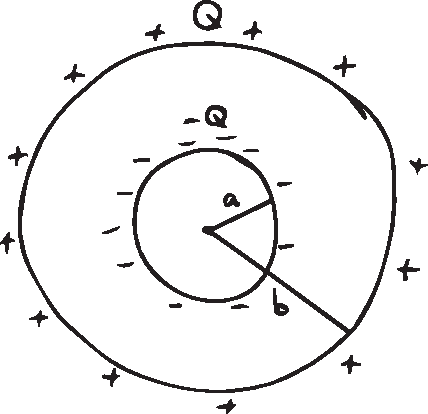
\includegraphics[scale=0.5]{07-condensateurs/figures/condensateur-spherique.pdf}
\end{center}

Deux armatures sphériques concentriques de rayon $a$ et $b$. Le champ
électrique est radial. On calcule la différence de potentiel de la plaque
négative à la plaque positive.

\begin{align*}
  \Delta V &= - \int_-^+ \vec{E} \cdot d\vec{s} \\
           &= - \int_-^+ E_r dr \\
           &= - \int_-^+ \frac{-kQ}{r^2} dr \\
           &= - \left. \frac{kQ}{r} \right|_-^+ \\
           &= -\frac{kQ}{b} - \frac{kQ}{a} \\
           &= k \frac{b - a}{ab} Q
\end{align*}

Donc
\begin{align*}
  C &= \frac{Q}{\Delta V} \\
    &= \frac{1}{k} \frac{ab}{b - a} \\
\end{align*}


\sectionline


\section{Circuits simples avec des condensateurs}

\marginpar{Tremblay \S 7.4}

\subsection*{Condensateurs en série}

\marginpar{15 minutes}

Si plusieurs condensateurs sont placés en série, est-ce que la capacité de
l'ensemble est plus grande, plus petite ou égale à la somme des capacités?

La charge accumulée sur chacun des condensateurs est la même parce les
armatures opposées doivent avoir des charges opposées, et chaque section du
circuit doit être électriquement neutre.

\begin{center}
  \includegraphics[scale=0.5]{07-condensateurs/figures/condensateur-serie.pdf}
\end{center}

De plus, la somme des différences de potentiel aux armatures de chacun des
condensateurs doit être la même que la différence de potentiel fournie par la
source. On a donc
\begin{align*}
  \Delta V &= \Delta V_1 + \Delta V_2 + \Delta V_3  \\
  \frac{q}{C_\mathrm{eq}} &= \frac{q}{C_1} + \frac{q}{C_2} + \frac{q}{C_3}  \\
  \frac{1}{C_\mathrm{eq}} &= \frac{1}{C_1} + \frac{1}{C_2} + \frac{1}{C_3}
\end{align*}



\subsection*{Condensateurs en parallèle}

\marginpar{15 minutes}

Dans le cas de condensateurs en parallèle, la charge accumulée sur chaque
condensateur n'est pas nécessairement la même, mais la ddp aux bornes de chaque
condensateur elle doit être identique. La charge qui sera accumulée sur un
condensateur équivalent aux trois condensateurs doit être la somme des charges
sur chaque condensateur.

\begin{center}
  \includegraphics[scale=0.5]{07-condensateurs/figures/condensateur-parallele.pdf}
\end{center}

On a donc
\begin{align*}
  q &= q_1 + q_2 + q_3  \\
  C_\mathrm{eq} \Delta V &= C_1 \Delta V + C_2 \Delta V + C_3 \Delta V  \\
  C_\mathrm{eq} &= C_1 + C_2 + C_3
\end{align*}


\section{Énergie dans un condensateur chargé}

\marginpar{Tremblay \S 7.5}
\marginpar{15 minutes}
\marginpar{Diapo}

On doit construire la configuration de charge, ie, calculer le travail
nécessaire pour amener chacune des charges à sa place sur le condensateur.

Considérons un condensateur avec une capacité $C$ dont les armatures sont
maintenues à une différence de potentiel $\Delta V$.

\begin{itemize}
  \item Si la charge sur la plaque est $q$, calculer l'énergie nécessaire pour
    amener une charge supplémentaire $dq$ sur la plaque.
  \item Déterminer l'énergie totale requise pour charger le condensateur avec
    une charge $Q$.
\end{itemize}


La différence de potentiel lorsque la charge est $q$ est
$$\Delta V = \frac{q}{C}$$
donc l'énergie requise pour amener une charge supplémentaire $dq$ est
\begin{align*}
  dU &= dq \Delta V \\
           &= \frac{q}{C} dq
\end{align*}
L'énergie totale est la somme des variations d'énergie pour chacune des petites
charges nécessaires pour faire passer la charge totale du condensateur de $0$ à
$Q$:
\begin{align*}
  \Delta U &= \int_0^Q \frac{q}{C} dq \\
           &= \left. \frac{q^2}{2C} \right|_0^Q \\
           &= \frac{Q^2}{2C}
\end{align*}


\sectionline


\section{Condensateurs et diélectriques}

\marginpar{Tremblay \S 7.7}

\paragraph{Objectif}

\begin{enumerate}
  \item L'étudiante connaîtra la définition de la constante diélectrique.
  \item L'étudiante comprendra comment l'introduction d'un diélectrique
    influence la capacité d'un condensateur.
\end{enumerate}

\marginpar{10 minutes}

Demander aux étudiants de résumer comment l'introduction d'un condensateur
entre les armatures d'un condensateur chargé affecte le champ électrique, la
différence de potentiel et la capacité.

Les éléments suivants devraient se retrouver dans la description.

\begin{itemize}
  \item Diélectrique se polarise ce qui crée un champ électrique dans le
    diélectrique dans la direction opposé au champ électrique causé par les
    armatures.
  \item Par le principe de superposition, le champ électrique total a un module
    inférieur à celui des armatures seules.
  \item La différence de potentiel diminue du même facteur puisqu'elle est
    proportionnelle au champ électrique.
  \item La charge sur les armatures est la même, mais la différence de
    potentielle est plus faible, donc la capacité a augmenté (car $C = Q/\Delta
    V$).
\end{itemize}


\subsection*{Constante diélectrique}

\marginpar{5 minutes}

Le champ électrique induit dans un diélectrique est en général proportionnel au
champ électrique externe
$$\vE_\text{diel} = \alpha \vE_\text{vide}$$
donc le champ électrique total est
$$\vE = \vE_\text{vide} + \vE_\text{diel} = (1 + \alpha) \vE_\text{vide}.$$
On définit la \textbf{constante diélectrique} comme
$$\kappa = \frac{1}{1 + \alpha}$$
ie
$$\vE = \frac{1}{\kappa} \vE_\text{vide}.$$
Par conséquent, la différence de potentiel entre les plaques chute d'un facteur
$\kappa$ et la capacité devient
$$C = \frac{Q}{\Delta V / \kappa} = \kappa C_\text{vide}.$$


\subsection*{Rigidité diélectrique}

Si le champ électrique externe appliqué sur un diélectrique est trop élevé, les
électrons seront arrachés aux atomes et un courant pourra traverser le
diélectrique. C'est ce qu'on appelle une \textbf{décharge}. Chaque matériau est
capable de supporter un champ électrique maximum qu'on appelle la
\textbf{rigidité diélectrique}. Le tableau ci-dessous donne la rigidité
diélectrique de quelques matériaux.

\marginpar{Diapo}
\begin{center}
\begin{tabular}{lS}
  \toprule
  Substance       &        {Rigidité diélectrique (\si{V/cm})}     \\
  \midrule
  Air             &  30000  \\
  Verre           &  100000 \\
  Polystyrène     &  197000 \\
  Papier ciré     &  500000 \\
  Diamant         &  20000000 \\
  \bottomrule
\end{tabular}
\end{center}


\subsection*{Exemple}

On construit le circuit suivant avec une pile de \SI{9}{V}. Le condensateur 1 a
une capacité $C_1 = \SI{45}{\micro\farad}$ et ses armatures sont séparées par
du vide. Les condensateurs 2 et 3 sont construits exactement de la même façon que le
condensateur 1 sauf que tout l'espace entre leurs armatures est rempli par
du germanium et du papier, respectivement. La constante diélectrique du
germanium est 16 alors que celle du papier est 3.

\begin{center}
\begin{circuitikz}
  \draw (0, 0) to[battery, l=$\SI{9}{\volt}$] (0, 3)
    to[C, l=$C_1$] (2, 3)
    to[C, l=$C_2$] (2, 0)
    to (0, 0);
  \draw (2, 3) to[short] (4, 3)
    to[C, l=$C_3$] (4, 0)
    to (2, 0);
\end{circuitikz}
\end{center}

\begin{enumerate}
  \item Déterminer la capacité équivalente à ces trois condensateurs.
  \item Déterminer la charge accumulée sur la plaque positive du condensateur 2.
  \item Déterminer l'énergie accumulée dans le condensateur 3.
\end{enumerate}


D'abord
\begin{align*}
  C_2 &= \kappa_\text{Ge} C_1 = 16C_1 = \SI{720}{\micro\farad} \\
  C_3 &= \kappa_\text{papier}C_1 = 3C_1 = \SI{135}{\micro\farad} \\
\end{align*}
$C_2$ et $C_3$ sont en parallèle donc
\begin{align*}
  C_{23} &= C_2 + C_3 \\
         &= \SI{855}{\micro\farad}
\end{align*}
$C_1$ est en série avec $C_{23}$ donc
\begin{align*}
  C_\text{eq} &= \frac{1}{\frac{1}{C_1} + \frac{1}{C_{23}}} \\
              &= \SI{42.8}{\micro\farad}
\end{align*}

La charge accumulée sur cette capacité équivalente serait la même que celle
accumulée sur $C_1$ et $C_{23}$. Donc
\begin{align*}
  Q_{23} &= C_\text{eq} \Delta V \\
         &= \SI{384.75}{\micro\coulomb}
\end{align*}
La différence de potentiel aux bornes de $C_2$ (et $C_3$) est donc
\begin{align*}
  \Delta V_{2} &= \frac{Q_{23}}{C_{23}} \\
               &= \SI{0.45}{\volt}
\end{align*}
d'où on peut déduire la charge accumulée sur $C_2$
\begin{align*}
  Q_2 &= C_2 \Delta V_2 \\
      &= \SI{324}{\micro\coulomb}
\end{align*}

L'énergie emmagasinée dans $C_3$ est obtenue par
\begin{align*}
  U_3 &= \frac{Q_3^2}{2C_3} = \frac{C_3 \Delta V_3^2}{2}  \\
      &= \SI{13.67}{\micro\joule}
\end{align*}



\subsection*{Condensateur qui explose}

Si on applique une différence de potentiel trop élevée aux armatures d'un
condensateur, le champ électrique entre les armatures deviendra plus grand que
la rigidité diélectrique du matériel isolant et on assistera à une décharge.
Très souvent, un condensateur qui subit une décharge explosera tel qu'illustré
dans le vidéo suivant \url{https://youtu.be/XBoaBwMRbnk?t=30}.


Dans un des cas, on voit un condensateur de \SI{470}{\micro\farad} qui explose.
Supposons qu'il a explosé à une tension de \SI{200}{\volt}. Quelle est la
quantité d'énergie qui peut être relâchée durant cette explosion?

\begin{align*}
  U &= \frac{C\Delta V^2}{2}  \\
    &= \SI{9.40}{J}
\end{align*}

C'est environ l'énergie d'un bloc de \SI{1}{kg} qui tombe d'une hauteur de
\SI{1}{m} sur le bout de votre doigt...




%\chapter{Champ magnétique}

\minisec{Objectif}

\begin{enumerate}
  \item L'étudiant saura comment interagissent des pôles magnétiques à
    proximité.
  \item L'étudiant pourra appliquer la loi de Biot-Savart au calcul du champ
    magnétique produit par un fil infini.
\end{enumerate}


\section{Rappels sur les aimants}

\marginpar{
  Tremblay \S 8.1

  Lafrance \S 8.1
}

Un aimant a un pôle nord et un pôle sud. Le pôle nord est attiré vers le pôle
nord géographique. Le pôle sud de l'aimant est attiré vers le pôle sud
géographique.

Si on place deux aimants à proximité, les pôles de même type se repoussent, les
pôles opposés s'attirent. Par conséquent, le nord géographique est un pôle sud
magnétique.

Un aimant peut attirer certains matériaux non aimantés. C'est semblable à ce
qu'on observait entre une tige chargée et un matériau neutre.

Si on coupe un aimant en deux, chaque morceau possède un pôle nord et un pôle
sud. Il est impossible d'isoler un pôle. Autrement dit, il n'existe pas (selon
nos connaissances actuelles) de monopôles magnétiques.

Les aimants sont entourés d'un champ magnétique.

Le champ magnétique se mesure en tesla (\si{T}) ou en gauss (\SI{1}{G} =
\SI{1e-4}{T}). Le champ magnétique terrestre est de l'ordre de \SI{0.5}{G}. Le
champ magnétique produit par une machine d'imagerie par résonance magnétique
est de l'ordre de \SI{2}{T}.


\subsection{Lignes de champ magnétique}

Comme pour le champ électrique, on peut définir des lignes de champ magnétique.
Elles possèdent les propriétés suivantes:
\begin{itemize}
  \item champ magnétique tangent aux lignes de champ
  \item grandeur du champ magnétique proportionnel à la densité de lignes de
    champ
  \item à l'extérieur d'un aimant, les lignes de champ vont du pôle nord vers
    le pôle sud.
\end{itemize}
Puisqu'il n'y a pas de monopôle magnétique, les lignes de champ forment
toujours des courbes fermées.



\minisec{Question}

Quelle est l'orientation du champ magnétique à l'intérieur d'un aimant?


\begin{diapobox}
\minisec{Exercice}

Pour chacune des situations suivantes, déterminer si les deux objets
s'attirent, se repoussent, ou n'exercent aucune force l'un sur l'autre. (Note:
les lignes de champ ne sont tracées que partiellement.)

\begin{center}
  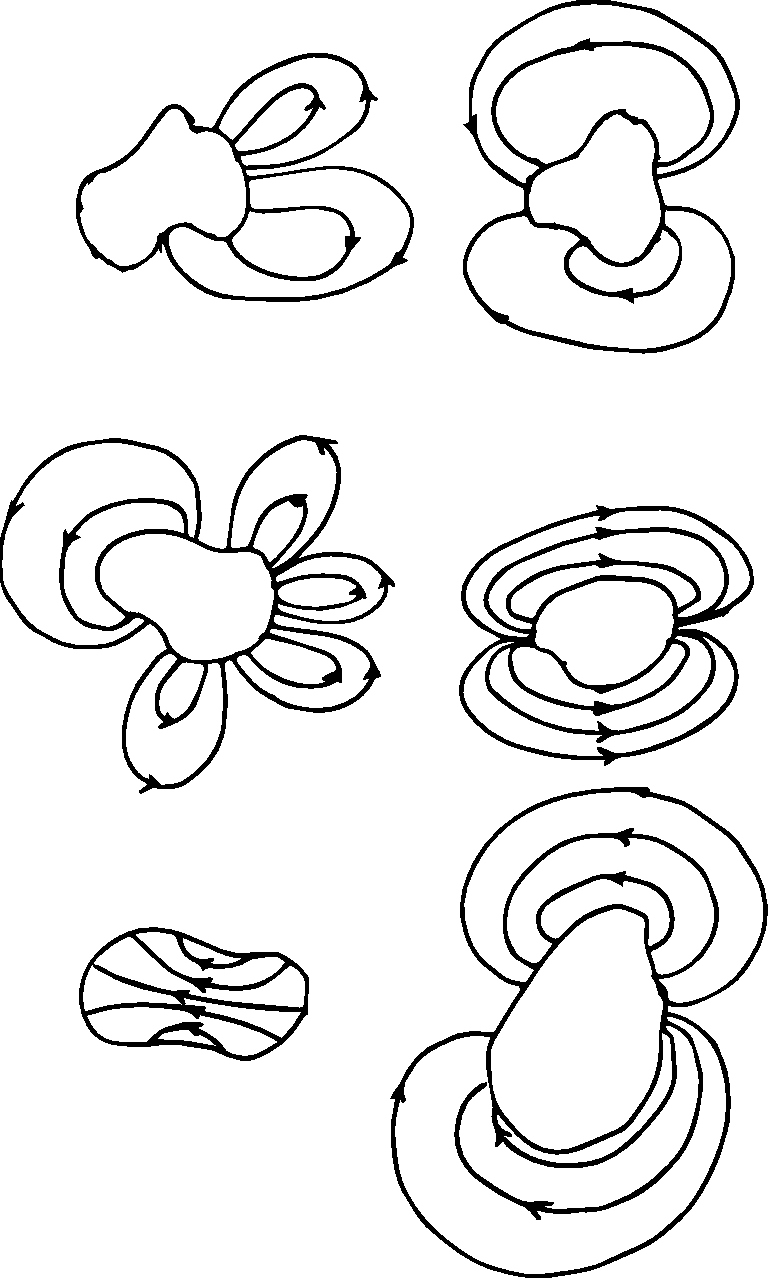
\includegraphics[scale=0.5]{08-champ-magnetique/figures/exercice-champ-magnetique1.pdf}
\end{center}

\end{diapobox}


\section{Source des champs magnétiques}

\marginnote{
  Lafrance \S 8.2
}

\minisec{Objectif}

\begin{enumerate}
  \item L'étudiant pourra appliquer la loi de Biot-Savart au calcul du champ
    magnétique produit par un fil infini.
\end{enumerate}


Démo avec un fil traversé d'un courant et une boussole. Montrer que la boussole
pointe toujours dans une direction tangente à un cercle centré sur le fil.

\begin{fondamentalbox}
  La source des champs magnétiques est le courant.
\end{fondamentalbox}

Les lignes de champ magnétique autour d'un long fil sont circulaire, centrées
sur le fil. L'orientation est obtenue à partir de la règle de la main droite.

\begin{diapobox}
  Quelle image illustre correctement le champ magnétique produit par le courant
  dans le fil?

  \begin{center}
    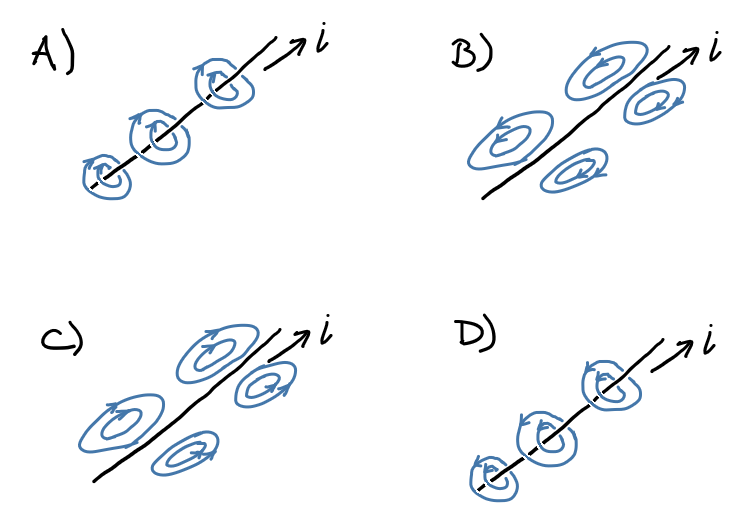
\includegraphics[scale=0.3]{08-champ-magnetique/figures/champ_fil_ex1.png}
  \end{center}

  \begin{center}
    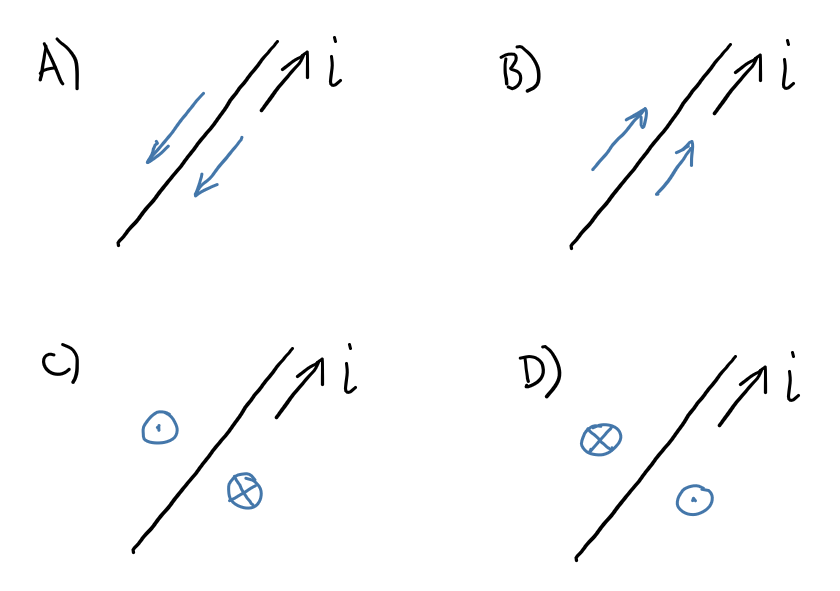
\includegraphics[scale=0.3]{08-champ-magnetique/figures/champ_fil_ex2.png}
  \end{center}
\end{diapobox}

\begin{diapobox}
  Quelle image illustre correctement le champ magnétique produit par le courant
  dans la boucle?

  \begin{center}
    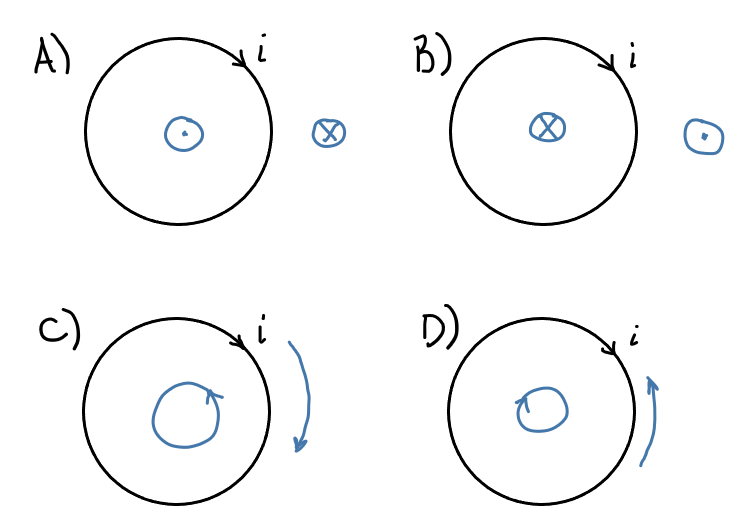
\includegraphics[scale=0.3]{08-champ-magnetique/figures/champ_boucle_ex1.png}
  \end{center}

  \begin{center}
    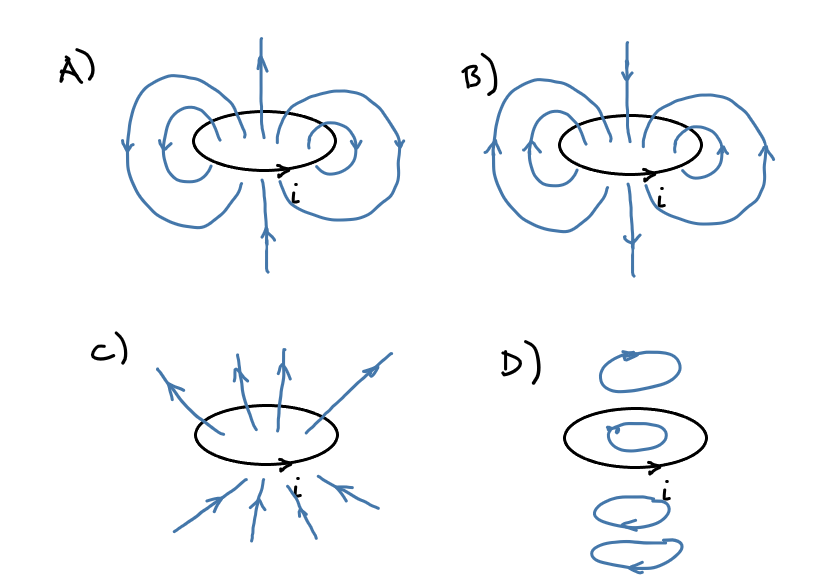
\includegraphics[scale=0.3]{08-champ-magnetique/figures/champ_boucle_ex2.png}
  \end{center}
\end{diapobox}

\begin{diapobox}
  \minisec{Champ magnétique d'un aimant}
  
  Quelle image illustre correctement les petites boucles de courant qui
  génèrent le champ d'un aimant?

  \begin{center}
    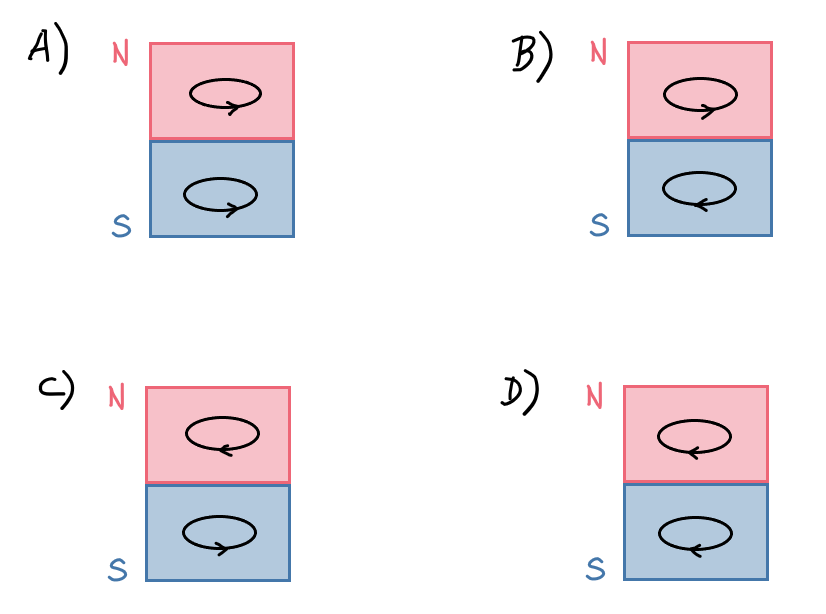
\includegraphics[scale=0.3]{08-champ-magnetique/figures/aimant_boucle.png}
  \end{center}

\end{diapobox}


\begin{fondamentalbox}
  \minisec{Loi de Biot-Savart}
  La loi de Biot-Savart est une formulation de ce qu'on vient
  d'observer.
  \marginnote{
  \begin{center}
    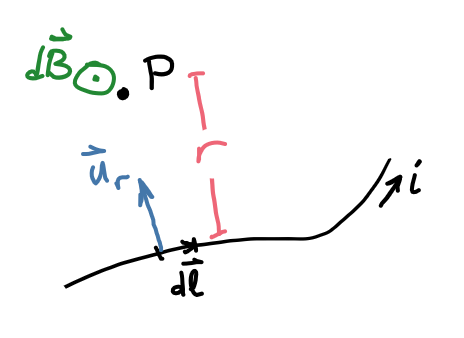
\includegraphics[scale=0.3]{08-champ-magnetique/figures/biot-savart.png}
  \end{center}
  }

  $$d\vB = \frac{\mu_0 I}{4\pi} \frac{d\vec{l} \times \vec{u}_r}{r^2} $$
  
  Le vecteur unitaire $\vec{u}_r$ va de la source du champ magnétique vers le
  point où le champ magnétique est calculé.
\end{fondamentalbox}

La constante $\mu_0$ s'appelle la \textbf{perméabilité du vide} (ou constante
magnétique) et vaut
$$\mu_0 = \SI{4\pi e-7}{Tm/A}$$


\begin{fondamentalbox}
  Le champ magnétique satisfait le principe de superposition, c'est-à-dire que
  le champ magnétique en un point est la somme vectorielle des champs produits
  par tous les courants à proximité.
\end{fondamentalbox}


\subsection*{Intermède mathématique : le produit vectoriel}

Le produit vectoriel entre deux vecteurs $\vu$ et $\vv$ est le vecteur de
grandeur
$$\abs{\vu \times \vv} = uv \sin\theta$$
orienté à \SI{90}{\degree} de $\vu$ et $\vv$ dans le sens donné par la règle de
la main droite.

\begin{diapobox}
  Classer les situations suivantes en ordre croissant de la grandeur du produit
  $\abs{\vu \times \vv}$.

  \begin{center}
    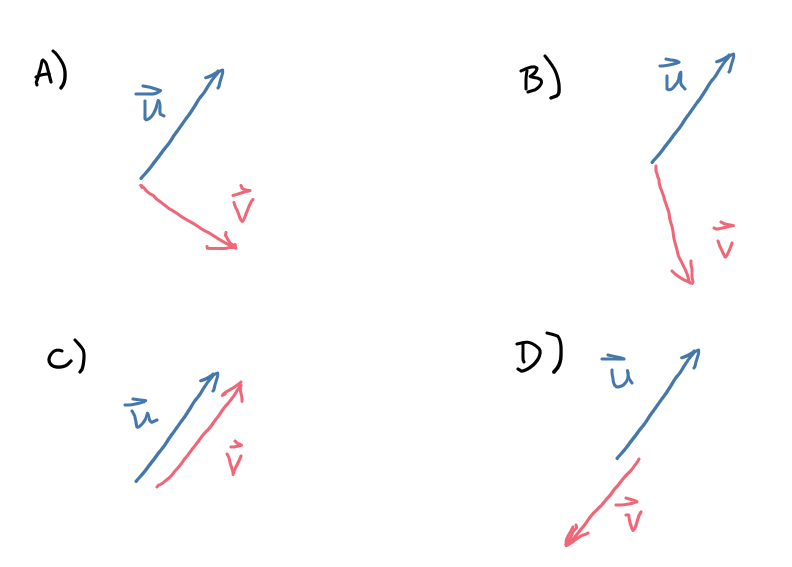
\includegraphics[scale=0.3]{08-champ-magnetique/figures/produit-vec_ex1.png}
  \end{center}
\end{diapobox}

Algébriquement, on peut calculer le produit vectoriel de $\vu =
\vecxyz{u_x}{u_y}{u_z}$ et $\vv = \vecxyz{v_x}{v_y}{v_z}$ comme suit
$$\vu \times \vv = \vecxyz{\left(u_y v_z - u_z v_y\right)}
                          {\left(u_z v_x - u_x v_z\right)}
                          {\left(u_x v_y - u_y v_x\right)}$$
Une approche complètement équivalente est de calculer le déterminant
$$
\vu \times \vv = \begin{vmatrix}
  \xhat  &  \yhat  &  \zhat  \\
  u_x    &  u_y    &  u_z    \\
  v_x    &  v_y    &  v_z
\end{vmatrix}
$$


\begin{diapobox}
\minisec{Exemple}

Calculer le produit vectoriel du vecteur $\vu = \vecxyz{3}{-2}{1}$ et du
vecteur $\vv$ dans le plan $xy$, de longueur $2$ et qui fait un angle de
\SI{30}{\degree} avec l'axe des $x$ positifs.
\end{diapobox}

\begin{reponsebox}
  On peut trouver les composantes de $\vv$ avec un peu de trigonométrie: $\vv =
  \vecxyz{\sqrt{3}}{1}{0}$. Ensuite, il suffit de calculer le produit
  \begin{align*}
    \vu \times \vv &= \begin{vmatrix}
      \xhat     &  \yhat  &  \zhat  \\
      3         &  -2     &  1      \\
      \sqrt{3}  &  1      &  0
    \end{vmatrix}  \\
  &= -\xhat + \sqrt{3} \yhat + (3 + 2 \sqrt{3})\zhat
  \end{align*}
\end{reponsebox}




\subsection*{Champ magnétique d'un fil infini}

Calculons le champ magnétique produit par un long fil rectiligne portant un
courant $i$, à une distance $a$ du centre du fil.
\marginnote{
  \begin{center}
    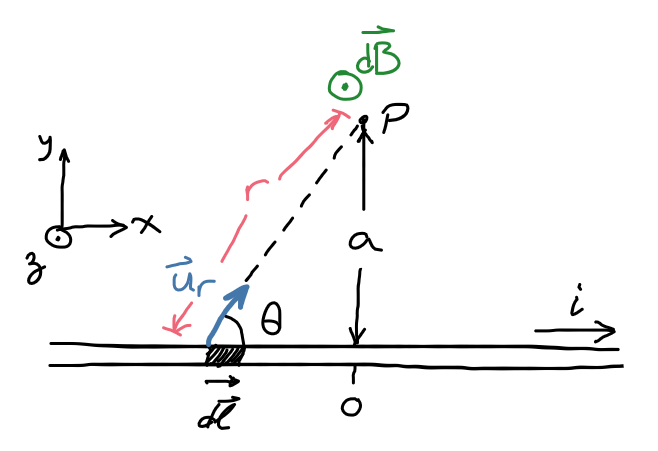
\includegraphics[scale=0.3]{08-champ-magnetique/figures/bs-champ-fil.png}
  \end{center}
}


Par la loi de Biot-Savart,
\begin{align*}
  d\vB &= \frac{\mu_0 i}{4\pi} \frac{d\vec{l} \times \vu_r}{r^2} \\
       &= \frac{\mu_0 i}{4\pi} \frac{dl \sin\theta \zhat}{r^2} \\
       &= \frac{\mu_0 i}{4\pi} \frac{dx a \zhat}{r^3}
\end{align*}
Par le principe de superposition, le champ total est obtenu en additionnant
les champs produits par tous les petits morceaux de fil:
\begin{align*}
  \vB &= \int_\mathrm{fil} \frac{\mu_0 i}{4\pi} \frac{dx a \zhat}{r^3} \\
      &= \frac{\mu_0 i a}{4\pi} \zhat \int_\mathrm{fil} \frac{dx}{\left(x^2 +
          a^2\right)^{3/2}}
\end{align*}
Pour couvrir le fil au complet, on intègre de $x = -\infty$ à $x = +\infty$.
\begin{align*}
  \vB &= \frac{\mu_0 i a}{4\pi} \zhat \int_{-\infty}^\infty
           \frac{dx}{\left(x^2 + a^2\right)^{3/2}}  \\
      &= \frac{\mu_0 i a}{4\pi} \zhat 
           \left[\frac{x}{a^2 \sqrt{x^2 + a^2}}\right]_{-\infty}^{\infty}  \\
      &= \frac{\mu_0 i}{4\pi a} \zhat 
           \left[\frac{x}{\sqrt{x^2 + a^2}}\right]_{-\infty}^{\infty}  \\
      &= \frac{\mu_0 i}{2\pi a} \zhat 
\end{align*}



\subsection*{Champ magnétique d'un arc de cercle}

Calculons le champ magnétique d'un fil en forme d'arc de cercle de rayon $R$
sous-tendant un angle $\alpha$ et portant un courant $i$, au centre de l'arc de
cercle.
\marginnote{
  \begin{center}
    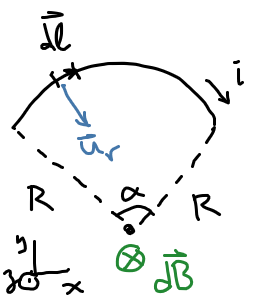
\includegraphics[scale=0.3]{08-champ-magnetique/figures/bs-champ-arc.png}
  \end{center}
}

Tous les petits morceaux du fil sont à la même distance du centre puisque c'est
un arc de cercle. L'angle entre $d\vec{l}$ et $\vu_r$ est toujours de
\SI{90}{\degree} parce que c'est un arc de cercle. Par la loi de Biot-Savart,
\begin{align*}
  d\vB &= \frac{\mu_0 i}{4\pi} \frac{d\vec{l} \times \vu_r}{r^2} \\
       &= \frac{\mu_0 i}{4\pi} \frac{dl \sin\theta (-\zhat)}{R^2} \\
       &= -\frac{\mu_0 i}{4\pi R^2} \zhat dl
\end{align*}
Par le principe de superposition, le champ total est obtenu en additionnant
les champs produits par tous les petits morceaux de fil:
\begin{align*}
  \vB &= \int_\mathrm{fil} -\frac{\mu_0 i}{4\pi R^2}\zhat dl  \\
      &= -\frac{\mu_0 i}{4\pi R^2}\zhat \int_\mathrm{fil} dl  \\
      &= -\frac{\mu_0 i}{4\pi R^2}\zhat R\alpha  \\
      &= -\frac{\mu_0 i \alpha}{4\pi R}\zhat
\end{align*}
On a intégré pour couvrir tout le fil, donc on obtient simplement longueur
totale du bout de fil.


\begin{diapobox}
  \subsection*{Machine d'imagerie par résonance magnétique}

  \marginnote{
    \footnotesize
    Aarnink, R. and Overweg, J. Magnetic Resonance Imaging a success story for
    superconductivity. Europhysics News, 43 4 (2012) 26-29. DOI:
    \url{https://doi.org/10.1051/epn/2012404}
  }
  Une machine d'imagerie par résonance magnétique permet de produire des images
  de l'intérieur du corps humain sans utiliser de technique invasive ni de
  rayonnement ionisant. Une machine typique produit un champ magnétique de
  \SI{1.50}{\tesla} au centre d'une bobine fait d'un supraconducteur
  (typiquement du nickel-titanium ou du nickel-étain). Si la bobine est faite
  de \num{10000} tours de fil et a un rayon de \SI{50}{\centi\meter}, quel est
  le courant qui doit circuler dans le fil?
\end{diapobox}

\begin{reponsebox}
  Calculons le champ magnétique d'une boucle de fil.
  \marginnote{
    \begin{center}
      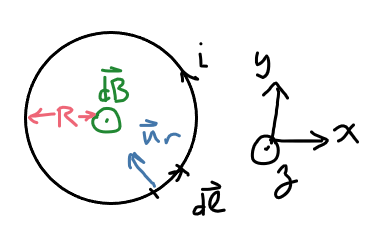
\includegraphics[scale=0.4]{08-champ-magnetique/figures/mri_figure_correcte.png}
    \end{center}
  }

  Tous les petits morceaux du fil sont à la même distance du centre puisque c'est
  un cercle. L'angle entre $d\vec{l}$ et $\vu_r$ est toujours de
  \SI{90}{\degree} parce que c'est un cercle. Par la loi de Biot-Savart,
  \begin{align*}
    d\vB_1 &= \frac{\mu_0 i}{4\pi} \frac{d\vec{l} \times \vu_r}{r^2} \\
         &= \frac{\mu_0 i}{4\pi R^2} \zhat dl
  \end{align*}
  Par le principe de superposition, le champ total est obtenu en additionnant
  les champs produits par tous les petits morceaux de fil:
  \begin{align*}
    \vB_1 &= \int_\mathrm{boucle} \frac{\mu_0 i}{4\pi R^2}\zhat dl  \\
        &= \frac{\mu_0 i}{4\pi R^2}\zhat \int_\mathrm{fil} dl  \\
        &= \frac{\mu_0 i}{4\pi R^2}\zhat 2\pi R  \\
        &= \frac{\mu_0 i}{2 R}\zhat
  \end{align*}
  On a intégré pour couvrir tout le fil, donc on obtient simplement longueur
  totale de la boucle. Chaque boucle génère un champ identique, donc le champ
  total, par le principe de superposition, est
  \begin{align*}
    \vB &= N\vB_1 \\
        &= \frac{\mu_0 i N}{2 R}\zhat
  \end{align*}
  Le champ total est connu, on cherche le courant donc
  \begin{align*}
    i &= \frac{2R B}{\mu_0 N}  \\
      &= \frac{2 \cdot \SI{50}{\centi\meter} \cdot \SI{1.5}{\tesla}}{4\pi
        \times 10^{-7} \cdot \num{10000}}  \\
      &= \SI{119.4}{\ampere}
  \end{align*}

  Si on utilisait du fil de cuivre de calibre 12 AWG
  (\SI{4}{\milli\meter\squared}), la résistance du fil serait de
  \begin{align*}
    R &= \frac{\rho \cdot 2 \pi R N}{A}  \\
      &= \SI{131.9}{\ohm}
  \end{align*}
  et la puissance dissipée dans le fil serait de
  \begin{align*}
    P &= Ri^2  \\
      &= \SI{1880}{\kilo\watt}
  \end{align*}
  C'est l'équivalent d'environ 450 cuisinières électriques qui fonctionnent à
  plein régime! De quoi faire des frites bien croustillantes!
\end{reponsebox}


\section{Champ magnétique d'un solénoïde}

\marginnote{
  Lafrance \S 8.6
}

Un solénoïde idéal est une succession de boucles de courant adjacentes formées
en enroulant un long fil autour d'un cylindre. On considère que le solénoïde a
une longueur infinie. Le champ magnétique peut être obtenu en appliquant le
principe de superposition pour additionner les champs produits par les boucles
individuelles. Le résultat est que le champ magnétique à l'extérieur du
solénoïde est nul et le champ magnétique à l'intérieur est uniforme et de
grandeur
$$B = \mu_0 i \frac{N}{L}$$
où $N/L$ est le nombre de tours par unité de longueur. La direction du champ
magnétique est obtenue en enroulant les doigts de la main droite dans la
direction du courant. Le pouce indique alors la direction du champ magnétique.


\begin{diapobox}
  Le réacteur à fusion nucléaire ITER est constitué d'une cavité toroïdale dans
  laquelle un plasma à haute température est confiné grâce à un champ
  magnétique de \SI{5.3}{\tesla}. Le champ magnétique est produit par un
  solénoïde toroïdal (un solénoïde dont les extrémités sont reliées ensembles).
  Le tore a un rayon d'environ \SI{6.2}{\meter} et les spires ont un rayon
  d'environ \SI{6.5}{\meter}. Le courant qui circule dans le câble est de
  \SI{68}{\kilo\ampere}. Quelle est la longueur de câble totale utilisée dans
  le solénoïde?
\end{diapobox}

\begin{reponsebox}
  Le nombre de ligne de champ par unité de longueur peut être obtenu par
  \begin{align*}
    B &= \mu_0 i n  \\
    n &= \frac{B}{\mu_0 i}  \\
      &= \SI{62.02}{\meter^{-1}}
  \end{align*}
  La longueur du solénoïde est
  \begin{align*}
    L &= 2\pi R  \\
      &= \SI{38.96}{\meter}
  \end{align*}
  où $R = \SI{6.2}{\meter}$. Le nombre total de tour est donc
  \begin{align*}
    N &= nL \\
      &= \frac{2\pi R B}{\mu_0 i}
  \end{align*}
  Chaque tour de câble a une longueur de $2\pi r$ où $r = \SI{6.5}{\meter}$. La
  longueur totale de câble est donc
  \begin{align*}
    d &= Nr  \\
      &= \frac{4\pi^2 rR B}{\mu_0 i}  \\
      &= \SI{98.68}{\kilo\meter}
  \end{align*}
\end{reponsebox}

%\chapter{Force magnétique}

\paragraph{Objectif}

\begin{enumerate}
  \item L'étudiant connaîtra l'expression de la force magnétique sur une
    particule chargée.
  \item L'étudiant pourra analyser un mouvement circulaire.
  \item L'étudiant comprendra le fonctionnement du sélecteur de vitesse, du
    spectromètre de masse.
\end{enumerate}



\section{Force magnétique sur une charge ponctuelle}

\marginnote{
  Lafrance \S 9.1, 9.2

  Tremblay \S 8.3, 8.4
}

\begin{fondamentalbox}
La force magnétique est proportionnelle à la charge, à la vitesse et au champ
magnétique. De plus, elle est perpendiculaire à la fois au champ magnétique et
à la vitesse.
$$\vF = q \vv \times \vB$$
\end{fondamentalbox}


\begin{diapobox}
  \marginnote{
    \begin{center}
      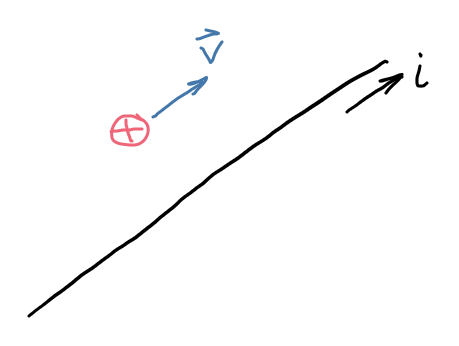
\includegraphics[scale=0.3]{09-force-magnetique/figures/proton_fil.png}
    \end{center}
  }
  Un proton a une vitesse parallèle à un long fil parcouru d'un courant $i$. La
  vitesse du proton est dans la même direction que le courant.
  Le proton 
  \begin{enumerate}
    \item se rapprochera du fil
    \item s'éloignera du fil
    \item continuera son chemin en ligne droite
  \end{enumerate}
\end{diapobox}

\begin{diapobox}
  \marginnote{
    \begin{center}
      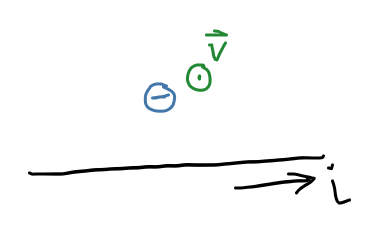
\includegraphics[scale=0.3]{09-force-magnetique/figures/electron_fil.png}
    \end{center}
  }
  Un électron a une vitesse perpendiculaire à un long fil parcouru d'un courant
  $i$. La force sur l'électron est 
  \begin{enumerate}
    \item vers le fil
    \item parallèle au fil
    \item nulle
    \item pointe en s'éloignant du fil
  \end{enumerate}
\end{diapobox}



\subsection*{Exemple - Mouvement circulaire}

On envoie des particules avec une vitesse horizontale de \SI{3.52e5}{m/s} dans
une région où existe un champ magnétique uniforme de \SI{1}{G} vers le bas. On
observe qu'à leur arrivée dans le champ magnétique, les particules tournent
dans le sens horaire lorsqu'on les regarde du dessus. Le rayon de leur
trajectoire est de \SI{2}{cm}.

\begin{enumerate}
  \item Déterminer le signe de la charge de ces particules.
  \item Déterminer le rapport $q/m$ pour ces particules.
  \item Déterminer la fréquence de leur mouvement.
\end{enumerate}


Signe est négatif car $\vv \times \vB$ pointe dans le sens anti-horaire donc la
charge doit être négative.

La force qui agit sur ces particules est
\begin{align*}
  \vF &= q\vv \times \vB \\
  F &= \abs{q} vB
\end{align*}
Par la deuxième loi de Newton,
\begin{align*}
  F &= \frac{mv^2}{R} \\ 
    &= \abs{q} vB
\end{align*}
Donc
\begin{align*}
  \frac{\abs{q}}{m} &= \frac{v}{RB} \\
  &= \SI{1.76e11}{C/kg}
\end{align*}

(Ce sont des électrons!)

Pour déterminer la fréquence, on veut savoir combien de tours sont effectués
chaque seconde.
\begin{align*}
  f &= \frac{v}{2\pi R} \\
    &= \SI{2.80e6}{Hz} = \SI{2.80}{MHz}
\end{align*}


\subsection*{Force de Lorentz}

Si une particule chargée est dans une région où il y a à la fois un champ
magnétique et un champ électrique, alors la force totale sur la particule est
la somme de la force électrique et de la force magnétique
$$\vF = q\vv \times \vB + q \vE$$



\subsection*{Exemple - Sélecteur de vitesse}

Des particules $\alpha$ sont envoyées dans une région où se trouvent un champ
électrique uniforme de \SI{236}{V/m} et un champ magnétique uniforme
perpendiculaire de \SI{155}{mT}. Quelle est l'énergie cinétique des particules
$\alpha$ qui continuent leur trajectoire en ligne droite?


La force est
\begin{align*}
  \vF &= q(\vv \times \vB + \vE) \\
      &= 0 \\
  \vv \times \vB &= -\vE \\
  v &= \frac{E}{B \sin \theta} \\
  v &= \SI{1522.58}{m/s} \\
  K &= \frac{1}{2} \times \SI{6.6465e-27}{kg} (\SI{1522.58}{m/s})^2 \\
    &= \SI{48.1}{meV}
\end{align*}


%\subsection*{Exemple - Spectromètre de masse}

%On considère un spectromètre de masse avec un champ magnétique de \SI{10}{G}.
%On envoie des ions +1 de nickel 58 (\SI{57.935}{u}) et de nickel 60
%(\SI{59.931}{u}).  Un sélecteur de vitesse s'assure que la vitesse de tous les
%ions est de \SI{1e5}{m/s}. Quelle est la distance entre les points où arrivent
%les deux isotopes de nickel?


%\begin{align*}
  %\frac{mv^2}{R} &= \abs{q} vB \\
  %R &= \frac{mv^2}{qvB} \\
  %D &= 2R_2 - 2R_1 \\
   %&= 2(m_2 - m_1) \frac{v}{qB} \\
   %&= \SI{0.414}{mm}
%\end{align*}


\section{Force magnétique sur les fils}

\marginnote{
  Lafrance \S 9.5
}

Si on a un fil parcouru d'un courant dans un champ magnétique, le fil subira
une force. En effet, les électrons se déplacent parce qu'il y a un courant.
Leur vitesse est la vitesse de dérive donc la force sur les charges mobiles est
\begin{align*}
  \vF_1 = q\vv \times \vB
\end{align*}
et la force totale est la somme de toutes les forces sur les porteurs de
charge soit
\begin{align*}
  \vF &= \sum \vF_1  \\
      &= \sum q \vv \times \vB
\end{align*}
Toutes les charges se déplacent à la même vitesse et se trouvent dans le même
champ magnétique donc on peut mettre en évidence le produit vectoriel
\begin{align*}
  \vF &= \left( \sum q \right) \vv \times \vB
\end{align*}
La quantité entre parenthèse est la charge totale qui se déplace qu'on peut
aussi écrire comme le produit du volume du fil $A\ell$, de la densité
volumique de charge $n$ et de la charge d'un porteur de charge
\begin{align*}
  \vF &= nA\ell q \vv \times \vB
\end{align*}
On se rappelle que le courant est définit comme $i = nAqv$ donc, en définissant
le vecteur $\vec{\ell}$ comme un vecteur de longueur $\ell$ qui pointe dans la
direction du courant,
\begin{align*}
  \vF = i\vec{\ell} \times \vB
\end{align*}

\begin{diapobox}
  \marginnote{
    \begin{center}
      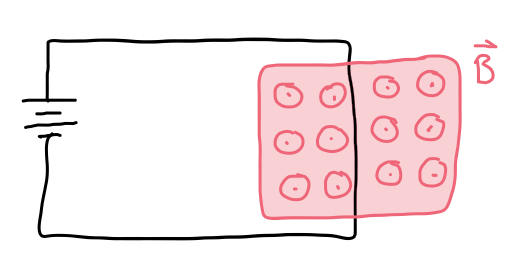
\includegraphics[width=3cm]{09-force-magnetique/figures/fil_dans_mag.png}
    \end{center}
  }
  Une section de fil de \SI{8}{\centi\meter} parcouru d'un courant de
  \SI{10}{\ampere} se trouve dans un champ magnétique uniforme de
  \SI{5}{\tesla}. Quelle est la force sur le fil?
\end{diapobox}

\begin{reponsebox}
  La force est vers la gauche (RMD) et de grandeur
  \begin{align*}
    F &= ilB \sin\SI{90}{\degree}  \\
      &= ilB  \\
      &= \SI{4}{\newton}
  \end{align*}
\end{reponsebox}


\begin{diapobox}
  \marginnote{
    \begin{center}
      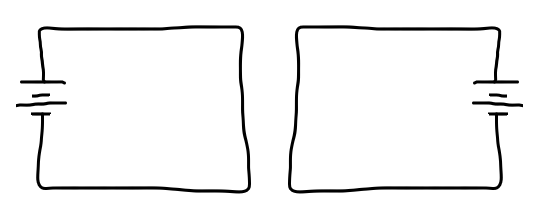
\includegraphics[width=3cm]{09-force-magnetique/figures/deux_fils.png}
    \end{center}
  }
  Une section de fil de \SI{8}{\centi\meter} parcouru d'un courant de
  \SI{10}{\ampere} se trouve à proximité d'une section de fil parallèle de même
  longueur parcouru d'un courant de \SI{5}{\ampere}. Les deux fils sont séparés
  d'une distance de \SI{2}{\centi\meter}.
  \begin{enumerate}
    \item Quelle est la force sur le fil de gauche?
    \item Quelle est la force sur le fil de droite?
  \end{enumerate}

\end{diapobox}

\begin{reponsebox}
  La force est vers la droite (RMD) et de grandeur
  \begin{align*}
    F &= i_1lB_2 \sin\SI{90}{\degree}  \\
      &= i_1lB_2  \\
      &= i_1 l \frac{\mu_0 i_2}{2\pi r}  \\
      &= \SI{4e-5}{\newton}
  \end{align*}
  La force sur le fil de droite est de même grandeur et vers la gauche, par la
  troisième loi de Newton.
\end{reponsebox}


\subsection{Moteur simple}

\marginnote{
  Lafrance \S 9.6
}

Un moteur est simplement une boucle (ou une bobine) de fil qui se trouve dans
un champ magnétique (produit par un aimant permanent ou un électroaimant). Le
fil est parcouru d'un courant dont la direction est changée à chaque demi-tour
grâce à un petit tour de passe passe mécanique qu'on appelle un commutateur.
L'idée est d'exercer un moment de force sur la boucle grâce au champ
magnétique.

\begin{diapobox}
  \marginnote{
    \begin{center}
      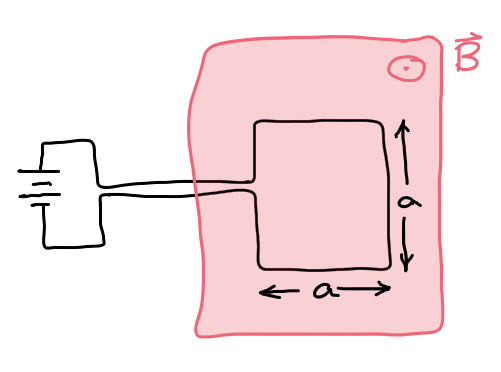
\includegraphics[width=3cm]{09-force-magnetique/figures/boucle_dans_mag.png}
    \end{center}
  }
  Déterminer la force magnétique sur la boucle suivante.

  \begin{enumerate}
    \item $iaB$
    \item $4iaB$
    \item $ia^2B$
    \item $0$
  \end{enumerate}

  Est-ce que la boucle tournera?

  \begin{enumerate}
    \item Oui, la partie du haut s'approchera de nous
    \item Oui, la partie du haut s'éloignera de nous
    \item Oui, la partie de droite s'approchera de nous
    \item Non
  \end{enumerate}
\end{diapobox}

\begin{diapobox}
  \marginnote{
    \begin{center}
      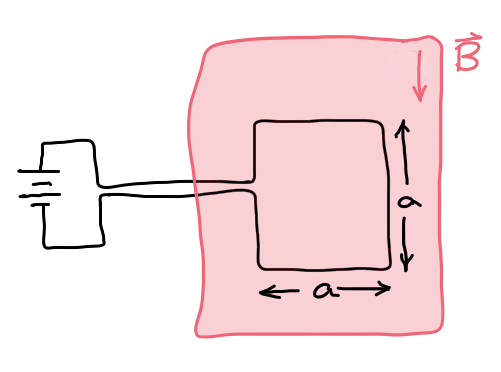
\includegraphics[width=3cm]{09-force-magnetique/figures/boucle_dans_mag_2.png}
    \end{center}
  }
  Déterminer la force magnétique sur la boucle suivante.

  \begin{enumerate}
    \item $iaB$
    \item $4iaB$
    \item $ia^2B$
    \item $0$
  \end{enumerate}

  Est-ce que la boucle tournera?

  \begin{enumerate}
    \item Oui, la partie du haut s'approchera de nous
    \item Oui, la partie du haut s'éloignera de nous
    \item Oui, la partie de droite s'approchera de nous
    \item Non
  \end{enumerate}
\end{diapobox}

%\chapter{Induction électromagnétique}


\paragraph{Objectif}

\begin{enumerate}
  \item L'étudiant connaîtra le concept de flux magnétique.
  \item L'étudiant connaîtra la loi de Lenz-Faraday.
\end{enumerate}


\section{Flux magnétique}

\marginnote{
  Lafrance \S 10.2
}

Le flux magnétique $\Phi_B$ est une mesure du nombre de lignes de champ qui
traversent une surface. Pour aider à comprendre, il est utile de faire une
analogie avec un fluide.


\begin{diapobox}

Classez les situations suivantes en ordre croissant de la quantité de liquide
qui passe à travers le cadre.

\begin{center}
  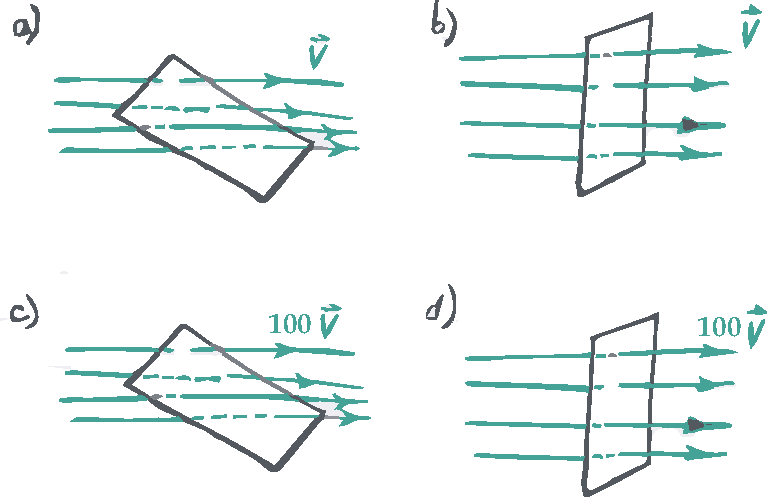
\includegraphics[scale=0.8]{10-induction-electromagnetique/figures/flux.pdf}
\end{center}

\end{diapobox}


\subsection*{Définition du flux magnétique}

On veut donc que le flux soit proportionnel à la composante du champ magnétique
perpendiculaire à la surface et à l'aire. Donc
$$\Phi_B = BA\cos\theta$$
Si on définit $\vec{A}$ comme un vecteur dont la longueur est l'aire de la
surface et qui est perpendiculaire à la surface, alors
$$\Phi_B = \vB \cdot \vec{A}$$

Si le champ magnétique n'est pas uniforme ou la surface n'est pas plane, alors
il faut considérer le flux à travers un petit morceau de surface puis intégrer
sur la surface en entier.
$$\Phi_B = \int_\mathrm{surface} \vB \cdot d\vec{A}$$

Les unités du flux sont des tesla mètres carrés ou des weber (Wb).


%\subsection*{Exercice --- Flux magnétique}

%Calculez le flux magnétique à travers une boucle rectangulaire placée
%radialement par rapport à un fil portant un courant $I = \SI{3}{A}$.

%\begin{center}
  %\begin{tikzpicture}[>=latex]
    %\draw[->] (0, 0) -- (0, 3.5) node[left] {$I$};
    %\draw (2, 1) rectangle (5, 2.5);
    %\draw[<->|] (0, 1.2) -- node[fill=white] {5 cm} (2, 1.2);
    %\draw[<->|] (0, 0.5) -- node[fill=white] {15 cm}(5, 0.5);
    %\draw[|<->|] (5.6, 2.5) -- node[fill=white] {4 cm} (5.6, 1);
  %\end{tikzpicture}
%\end{center}

%Le champ du fil est
%$$B = \frac{\mu_0 I}{2 \pi r}$$
%entrant dans la page.
%\begin{align*}
  %\Phi_B &= \int_a^b \frac{\mu_0 I}{2 \pi r} h dr \\ 
         %&= \frac{\mu_0 Ih}{2\pi} [\ln(a) - \ln(b)] \\
         %&= \SI{2.64e-6}{Tm^2}
%\end{align*}


\begin{diapobox}
  \minisec{Exercice flux magnétique}
  \marginnote{
    \begin{center}
      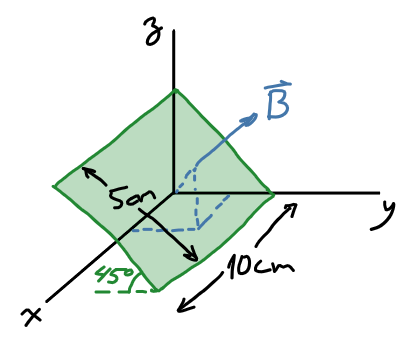
\includegraphics[width=4cm]{10-induction-electromagnetique/figures/flux-boucle-1.png}
    \end{center}
  }
  La boucle ci-contre est dans une région où se trouve un champ magnétique
  uniforme $\vB = \left(\vecxyz{1}{1}{1}\right) \si{G}$. Quel est le flux
  magnétique à travers la boucle?
\end{diapobox}

\begin{reponsebox}
  Le vecteur surface est $\vec{A} = \frac{ab}{\sqrt{2}}(\yhat + \zhat)$. Le
  flux est donc
  \begin{align*}
    \Phi_B &= \vB \cdot \vec{A}  \\
           &= \frac{ab}{\sqrt{2}}  (1 + 1) \si{G}  \\
           &= 5 \sqrt{2} \times 10^{-7} \si{\weber}
  \end{align*}
\end{reponsebox}




\section{Loi de Faraday}

\marginnote{
  Lafrance \S 10.3, 10.4
}

Une observation que vous avez faite au laboratoire est qu'un champ magnétique
variable induit une f.é.m. dans une boucle de fil conducteur. Faraday a
découvert que la f.é.m. induite est proportionnelle au taux de variation du
flux magnétique.
\begin{fondamentalbox}
  \minisec{Loi de Faraday}
  $$\emf = -\frac{d\Phi_B}{dt}$$
\end{fondamentalbox}
Le signe positif de la fém correspond à la direction des doigts de la main
droite lorsque le pouce est dans la direction du champ magnétique externe.

Dans le cas d'un champ uniforme et d'une boucle plate, on a
\begin{align*}
  \frac{d\Phi_B}{dt} &= \frac{d}{dt} \vB \cdot \vec{A} \\
                     &= \frac{dB}{dt} A\cos\theta + B \frac{dA}{dt} \cos\theta
                     + BA \frac{d\cos\theta}{dt} \\
                     &= \frac{dB}{dt} A\cos\theta + B \frac{dA}{dt} \cos\theta
                     - BA \sin\theta \frac{d\theta}{dt}
\end{align*}
Donc on peut obtenir une fém induite en faisant varier soit la grandeur du
champ, soit l'aire, soit l'orientation de la boucle dans l'espace.

Le courant dans la boucle peut circuler dans deux directions différentes. Pour
déterminer la direction, on utilise la loi de Lenz:

\begin{fondamentalbox}
  \minisec{Loi de Lenz}
  Le courant induit dans la boucle circule de façon à générer un champ
  magnétique induit qui s'oppose à la variation de flux magnétique.
\end{fondamentalbox}


\begin{diapobox}
  \minisec{Exemple d'application de la loi de Lenz}

  \marginnote{
    \begin{center}
      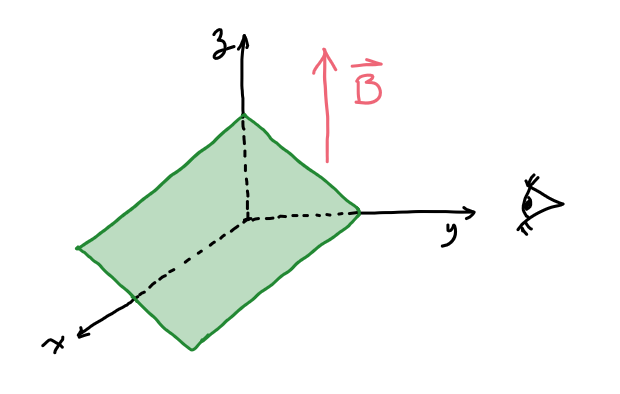
\includegraphics[width=4cm]{10-induction-electromagnetique/figures/boucle_oeil.png}
    \end{center}

    \begin{center}
      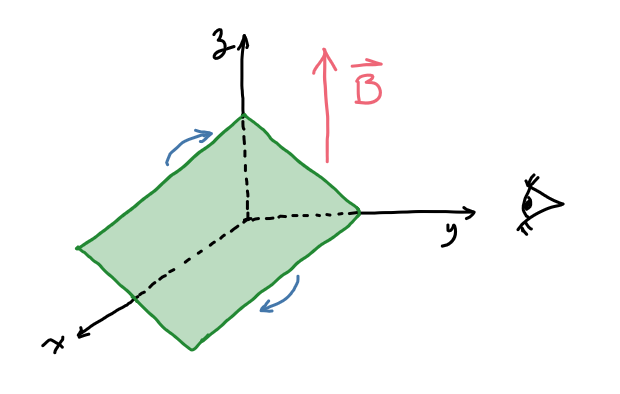
\includegraphics[width=4cm]{10-induction-electromagnetique/figures/boucle_oeil_tourne.png}
    \end{center}
  }

  Une boucle de fil se trouve dans un champ magnétique uniforme tel qu'illustré
  sur le dessin ci-dessous.

  La grandeur du champ magnétique augmente avec le temps. Quelle est la
  direction du courant induit dans la boucle?

  La grandeur du champ magnétique diminue avec le temps. Quelle est la
  direction du courant induit dans la boucle?

  La boucle tourne dans le sens indiqué sur le dessin. Quelle est la direction
  du courant induit dans la boucle?

  \begin{enumerate}
    \item sens horaire
    \item sens anti-horaire
    \item aucun courant induit
  \end{enumerate}

\end{diapobox}


\begin{diapobox}
  \minisec{Loi de Faraday - Champ magnétique variable}
  \marginnote{
    \begin{center}
      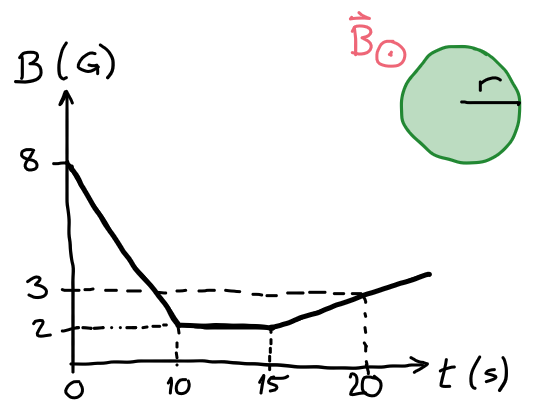
\includegraphics[width=4cm]{10-induction-electromagnetique/figures/champ_variable.png}
    \end{center}
  }
  Une bobine circulaire de \SI{5}{\centi\meter} de rayon comportant \num{50}
  tours se trouve dans un champ magnétique uniforme dont la grandeur varie dans
  le temps tel qu'illustré dans le graphique ci-dessous.

  Déterminez la f.é.m. induite et la direction du courant à
  \begin{enumerate}
    \item $t = \SI{5}{\second}$
    \item $t = \SI{11}{\second}$
    \item $t = \SI{20}{\second}$
  \end{enumerate}
\end{diapobox}

\begin{reponsebox}
  Le flux est
  \begin{align*}
    \Phi_B = \pi r^2 B N
  \end{align*}
  car le champ magnétique et le vecteur normal à la boucle sont dans la même
  direction. La f.é.m. est donc
  \begin{align*}
    \emf &= -\frac{d \Phi_B}{dt}  \\
         &= -\pi r^2 N \frac{dB}{dt}
  \end{align*}
  Puisque la grandeur du champ magnétique est linéaire par morceau, le taux de
  variation est simplement la pente du segment de droite approprié. On a donc
  \begin{align*}
    \emf_5 &= -\pi r^2 N \frac{\SI{2}{G} - \SI{8}{G}}{\SI{10}{\second} -
              \SI{0}{\second}}  \\
           &= \SI{0.2356e-4}{\volt}
  \end{align*}
  Puisque le champ magnétique diminue, le flux diminue et le champ induit doit
  être dans la même direction que le champ externe et le courant est donc dans
  le sens anti-horaire par la RMD.


  À $t = \SI{11}{\second}$, le champ magnétique ne varie pas, donc il n'y a pas
  de f.é.m. induite.

  Enfin,
  \begin{align*}
    \emf_{20} &= -\pi r^2 N \frac{\SI{3}{G} - \SI{2}{G}}{\SI{20}{\second} -
              \SI{15}{\second}}  \\
           &= \SI{-0.07854e-4}{\volt}
  \end{align*}
  Puisque le champ magnétique externe augmente, le flux augmente et le champ
  induit doit être dans la direction opposée au champ externe. Le courant est
  donc dans le sens horaire par la RMD. 

\end{reponsebox}



\begin{diapobox}
  \minisec{Générateur linéaire}

  Un cadre métallique fixe sert de support à une tige métallique mobile. La tige
  se déplace vers la droite à \SI{20}{cm/s} et sa longueur est de \SI{35}{cm}. Le
  champ magnétique externe est uniforme de \SI{120}{G}.
  Si la résistance de la boucle est de \SI{4}{\ohm}, déterminer le courant induit
  dans la boucle.

  \begin{center}
  \begin{tikzpicture}[>=latex]
    \draw[thick] (5, 0) -- (0, 0) -- (0, 3) -- (5, 3);
    \draw[thick, fill] (2, -0.15) rectangle (2.15, 3.15);
    \draw[->] (2.25, 1.5) -- ++(1, 0) node[right] {$\vec{v}$};
    \draw[|<->|] (-0.4, 0) -- node[fill=white] {$L$} (-0.4, 3);
    \draw (3, 3.5) circle (0.15);
    \draw (2.894, 3.394) -- (3.1061, 3.6061);
    \draw (2.894, 3.6061) -- (3.1061, 3.394);
    \node at (3.3, 3.8) {$\vec{B}$};
  \end{tikzpicture}
  \end{center}
\end{diapobox}

\begin{reponsebox}
Le flux magnétique dans la boucle change parce que l'aire change. Dans un
intervalle de temps $dt$, l'aire change de
$$dA = Lvdt.$$
Autrement dit
$$\frac{dA}{dt} = Lv$$
Le flux magnétique est
\begin{align*}
  \abs{\Phi_B} &= BA
\end{align*}
donc le changement de flux est 
\begin{align*}
  \abs{\frac{d\Phi_B}{dt}} &= B \frac{dA}{dt} \\
      &= BLv
\end{align*}
Par conséquent
\begin{align*}
  \emf &= BLv \\
  I &= \frac{BLv}{R} \\
    &= \SI{0.210}{mA}
\end{align*}
Puisque l'aire augmente, le flux augmente donc la fém induite doit produire un
champ magnétique dans la direction opposée à celle du champ externe. Le courant
circule donc dans le sens anti-horaire.
\end{reponsebox}


\minisec{Générateur}

Une boucle rectangulaire tourne à vitesse angulaire $\omega$ dans un champ
magnétique externe $\vB$. Un courant alternatif sera produit dans la boucle.
La position angulaire de la boucle est donnée par
\begin{align*}
  \theta = \theta_0 + \omega t
\end{align*}
Le flux magnétique est
\begin{align*}
  \Phi_B = BA \cos(\theta_0 + \omega t)
\end{align*}
donc
\begin{align*}
  \emf = -\frac{d\Phi_B}{dt} = BA\omega \sin(\theta_0 + \omega t)
\end{align*}

Quelle est la tension efficace?

\begin{align*}
  \emf_\mathrm{eff} &= \frac{\emf_m}{\sqrt{2}} \\
                    &= \frac{BA\omega}{\sqrt{2}} 
\end{align*}


%\include{cours11/planif11}
%\include{cours12/planif12}
%\include{cours13/planif13}
%\include{cours14/planif14}
%\include{cours15/planif15}
%\include{cours16/planif16}
%\include{cours17/planif17}
%\include{cours18/planif18}
%\include{cours19/planif19}
%\include{cours20/planif20}
%\include{cours21/planif21}
%\include{cours23/planif23}
%\include{cours25/planif25}
%\include{cours26/planif26}
%\include{cours27/planif27}
%\include{cours30/planif30}
%\include{cours31/planif31}
%\include{cours32/planif32}
%\include{cours34/planif34}

\end{document}
